\documentclass[journal]{IEEEtran}

\usepackage[utf8]{inputenc}
\usepackage[T1]{fontenc}
\usepackage{cite}
\usepackage{url}
\usepackage{booktabs}
\usepackage{amsfonts}
\usepackage{microtype}
\usepackage[table,xcdraw]{xcolor}
\usepackage{tabularx}
\usepackage{graphicx}
\usepackage{multirow}
\usepackage{tikz}
\usetikzlibrary{tikzmark,calc}

\definecolor{phaseLocalBg}{HTML}{DBEAFE}   % pale blue   (tint of #2563EB)
\definecolor{phaseConsolBg}{HTML}{D1FAE5}  % pale green  (tint of #059669)
\usepackage{amsmath}
\usepackage{amssymb}
\usepackage{mathtools}
\usepackage{amsthm}
\usepackage{algorithm}
\usepackage{algorithmic}
\usepackage[hidelinks]{hyperref}
\usepackage[capitalize,noabbrev]{cleveref}
\newcommand{\legendBox}[1]{{\color{#1}\rule[-0.05ex]{1.2em}{1.0ex}}}

% Make hyperref and algorithmic work together
\renewcommand{\theHalgorithm}{\arabic{algorithm}}

%%%%%%%%%%%%%%%%%%%%%%%%%%%%%%%%
% THEOREMS
%%%%%%%%%%%%%%%%%%%%%%%%%%%%%%%%
\theoremstyle{plain}
\newtheorem{theorem}{Theorem}
\newtheorem{proposition}[theorem]{Proposition}
\newtheorem{lemma}[theorem]{Lemma}
\newtheorem{corollary}[theorem]{Corollary}
\theoremstyle{definition}
\newtheorem{definition}[theorem]{Definition}
\newtheorem{assumption}[theorem]{Assumption}
\theoremstyle{remark}
\newtheorem{remark}[theorem]{Remark}

% ============================================================
% HTCL Notation Macros
% For: Hierarchical Taylor Series Continual Learning
% ============================================================

% ============================================================
% MODEL PARAMETERS
% ============================================================
\newcommand{\wh}[1]{\mathbf{w}_{#1}}            % Hierarchical model at level #1
\newcommand{\wl}{\mathbf{w}_{\ell}}             % Local model weights  
\newcommand{\w}{\mathbf{w}}                     % General weights
\newcommand{\wopt}{\mathbf{w}^{*}}              % Optimal weights
\newcommand{\whT}[2]{\mathbf{w}_{#1}^{(#2)}}    % Hierarchical weights level #1 at time #2
\newcommand{\wlT}[1]{\wl^{(#1)}}                % Local weights at time #1

% ============================================================
% TASKS AND GROUPS
% ============================================================
\newcommand{\T}{\mathbb{T}}                    % Task set
\newcommand{\tsk}{\tau}                         % Individual task
\newcommand{\G}{\mathrm{G}}                    % Task group
\newcommand{\D}{\mathrm{D}}                    % Dataset
\newcommand{\Dist}{\mathbb{P}}                 % Data distribution

% ============================================================
% DATA
% ============================================================
\newcommand{\x}{\mathbf{x}}                     % Input data
\newcommand{\y}{y}                              % Labels

% ============================================================
% PERMUTATIONS
% ============================================================
\newcommand{\perm}{\pi(t)}                         % Individual permutation
\newcommand{\permset}{\Pi(t)}                      % Set of all permutations
\newcommand{\permopt}{\pi^{*}}                  % Optimal permutation
\newcommand{\gpermset}{\varsigma}               % Intra-group permutation set
\newcommand{\gperm}{\sigma}                     % group perm

% ============================================================
% LOSS FUNCTIONS
% ============================================================
\newcommand{\loss}{\mathrm{L}}                 % Task loss function
\newcommand{\J}{\mathcal{J}}                    % Cumulative/Expected loss

% ============================================================
% DERIVATIVES
% ============================================================
% Note: Gradient and Hessian use \mathbf{g} and \mathbf{H} directly in text
% No macros defined to avoid conflicts with other packages

% ============================================================
% REGULARIZATION AND UPDATES
% ============================================================
\newcommand{\reg}{\lambda}                      % Regularization coefficient
\newcommand{\Dw}{\Delta\mathbf{w}}              % Weight change
\newcommand{\Dd}{\Delta\mathbf{d}}              % Local-hierarchical difference

% ============================================================
% METRICS AND EVALUATION
% ============================================================
\newcommand{\Acc}{A}                            % Accuracy/performance metric
\newcommand{\Eval}{\mathrm{Eval}}               % Evaluation function
\newcommand{\TrainSeq}{\mathrm{TrainSeq}}       % Sequential training function

% ============================================================
% HIERARCHY
% ============================================================
\newcommand{\hier}{\mathcal{H}}                 % Hierarchy set
\newcommand{\nlev}{L}                           % Number of hierarchical levels

% ============================================================
% DIMENSIONS AND COUNTS
% ============================================================
\newcommand{\ntasks}{t}                         % Number of tasks
\newcommand{\ngroups}{m}                        % Number of groups
\newcommand{\gsize}{k}                          % Group size
\newcommand{\pdim}{d}                           % Parameter dimension
\newcommand{\ncatch}{N_{\mathrm{catch}}}        % Catch-up iterations

% ============================================================
% OPERATORS
% ============================================================
\newcommand{\E}{\mathbb{E}}                     % Expectation
\newcommand{\R}{\mathbb{R}}                     % Real numbers
\DeclareMathOperator*{\argmin}{arg\,min}
\DeclareMathOperator*{\argmax}{arg\,max}

% ============================================================
% END OF MACROS
% ============================================================

\begin{document}

\title{Mitigating Task-Order Sensitivity and Forgetting via Hierarchical Second-Order Consolidation}

% TODO: fill in full author list and affiliations
\author{Protik~Nag,~\IEEEmembership{Student Member,~IEEE,}
        Second~Author,
        and~Third~Author% <-this % stops a space
\thanks{P. Nag is with the Department of Computer Science and Engineering, University of South Carolina, Columbia, SC 29208 USA (e-mail: protiknag08@gmail.com).}%
\thanks{Manuscript received Month DD, 2026; revised Month DD, 2026.}}

\markboth{IEEE Transactions on Neural Networks and Learning Systems,~Vol.~XX, No.~X, Month~2026}%
{Nag \MakeLowercase{\textit{et al.}}: Hierarchical Second-Order Consolidation for Continual Learning}

\maketitle

\begin{abstract}
We introduce Hierarchical Taylor Series-based Continual Learning (HTCL), a framework that reduces the sensitivity of continual learners to random task ordering by coupling fast local adaptation with conservative, second-order global consolidation. Rather than searching for the globally optimal task sequence, which is intractable due to factorial complexity, HTCL targets order robustness by partitioning the task stream into small groups and integrating their best per-group solutions through a Hessian-regularized Taylor expansion. We theoretically derive a unique closed-form consolidation update and establish a performance bound on HTCL's expected accuracy, showing that it improves over random task orderings. The approach naturally extends to an $L$-level hierarchy, enabling multiscale knowledge integration in a manner not supported by conventional single-level CL systems. Across a wide range of datasets and replay and regularization baselines, HTCL acts as a model-agnostic consolidation layer that consistently enhances performance, yielding mean accuracy gains of $7\%$ to $25\%$ while reducing the standard deviation of final accuracy by up to $68\%$ across random task permutations.
\end{abstract}

\begin{IEEEkeywords}
Continual learning, catastrophic forgetting, task-order sensitivity, second-order optimization, Taylor series expansion, hierarchical consolidation.
\end{IEEEkeywords}

\section{Introduction}\label{sec:intro}

\begin{figure}[!t]
  \centering  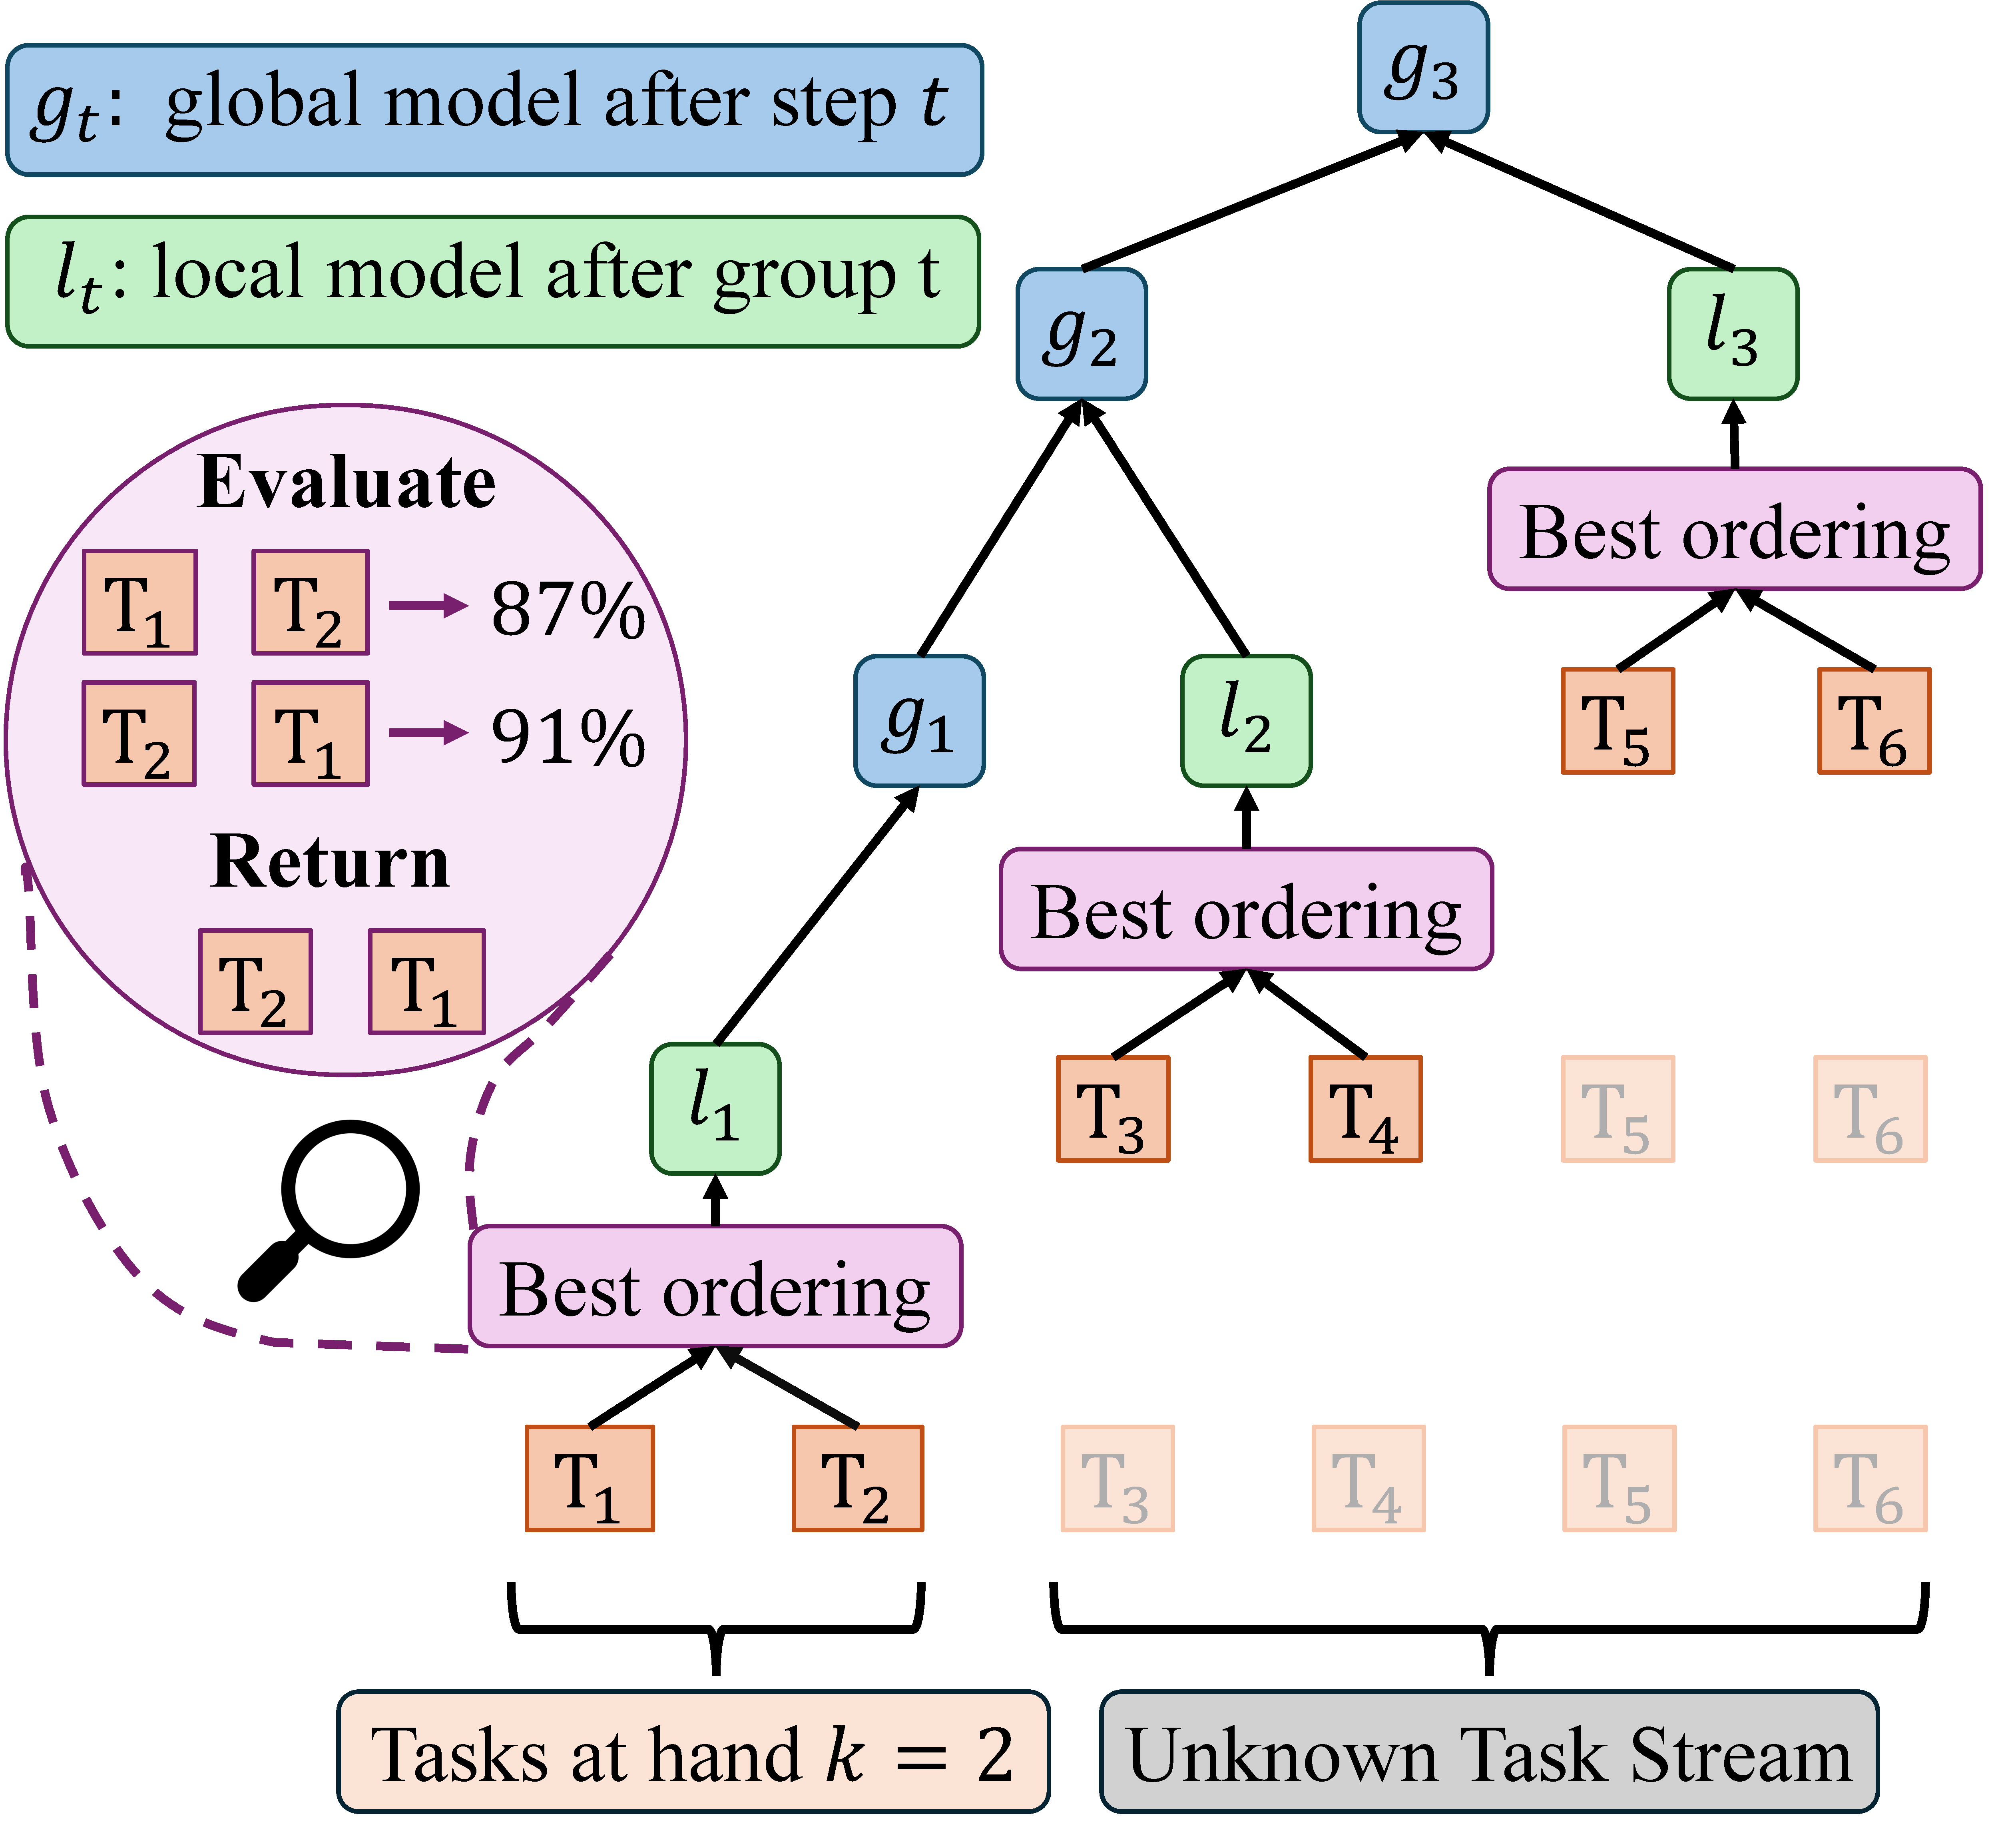
\includegraphics[width=\columnwidth]{figures/hier-explanation-fig.pdf}
  \caption{\textbf{Overview of HTCL with group size $k=2$.} The task stream is partitioned into disjoint groups (faded tasks denote the future stream)}
  \label{fig:hier-explanation}
\end{figure}

Continual learning (CL) aims to enable neural networks to acquire knowledge sequentially without catastrophically forgetting previously learned information~\cite{kirkpatrick2017overcoming, parisi2019continual}. This capability,  studied extensively~\cite{rebuffi2017icarl, zenke2017continual, fernando2017pathnet}, encounters a fundamental challenge: \emph{task-order sensitivity}. In particular, empirical studies report substantial increases in performance variance, up to $22\%$, in real-world deployments, where task sequences are rarely under the practitioner’s control~\cite{de2021continual} (see Appendix~\ref{app:impact-example} and related experiments in~\cite{bell2022effect, riemer2018learning}). %

\emph{Such variance is unacceptable in practice}. For instance, a medical diagnosis model's performance cannot depend on the order in which the diseases are introduced to it during training. A naive solution to this problem is to train the model over all possible task orderings and select the best one. However, such exhaustive training is NP-hard since $n$ tasks will require training the model on $n!$ permutations. \emph{Therefore, it is infeasible to find the best order of tasks over which to train.}

\begin{figure}[!t]
  \centering
  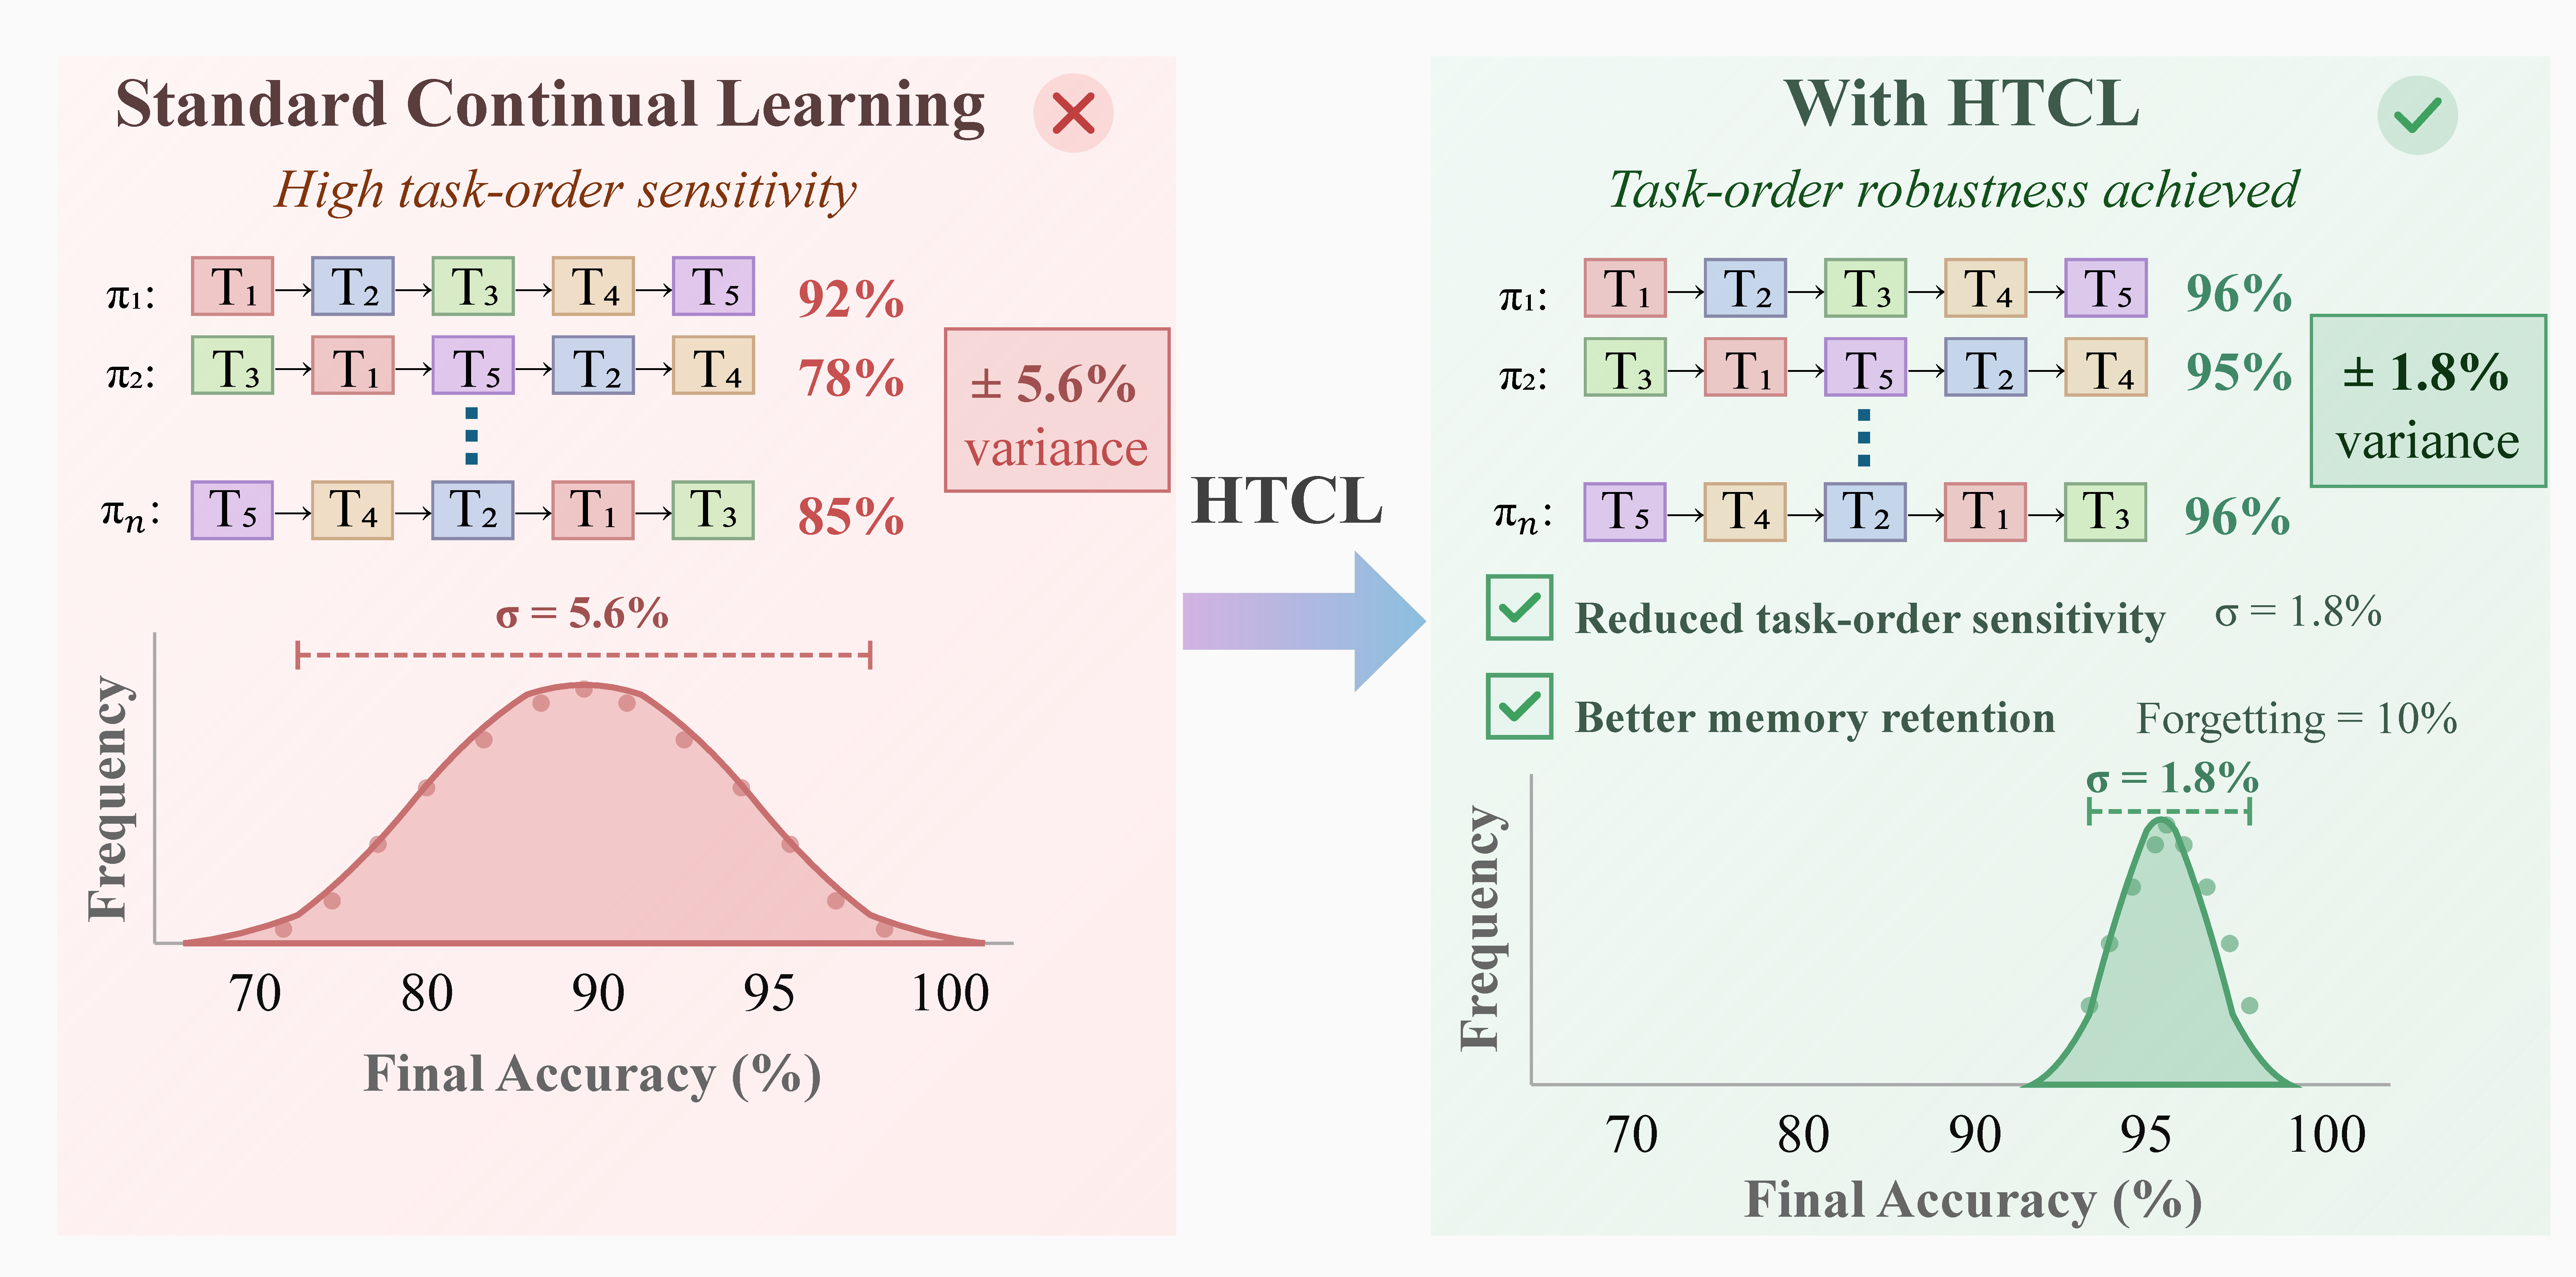
\includegraphics[width=\columnwidth]{figures/first-page.pdf}
  \caption{Task-order sensitivity in CL and its mitigation via HTCL. \textbf{Left:} Standard CL methods exhibit high sensitivity to task ordering. \textbf{Right:} HTCL achieves consistent performance regardless of task ordering, producing a narrow accuracy distribution.}
  \label{fig:new-cl-goal}
\end{figure}
Alternatively, it is more attractive to understand ``\emph{how to increase the robustness of the model in the presence of arbitrary task order?}"  To this end, we introduce \textbf{Hierarchical Taylor Series-based Continual Learning (HTCL)}. Our hierarchical framework imagines two levels of sequential consolidation steps as shown in Figure \ref{fig:hier-explanation}. At the first level, we collect $k$ tasks from the CL task sequence. Using these $k$ tasks, we determine the best task order and train a local model. Next, at level 2, we collect two local models from level one and consolidate them using a second order update rule. This consolidated model is then used as the initial condition for the next sequence of $k$ tasks, and the two-level training process is repeated. This simple two-step approach incorporates two integral strategies, \emph{a divide and conquer strategy and a hierarchical consolidation strategy.} %

As illustrated in Figure \ref{fig:hier-explanation}, in the first level, our approach focuses on a small group of $k$ tasks collected online. Within these $k$ tasks, HTCL is \emph{model- and CL-method-agnostic}: one may employ any existing CL method, utilize any model architectures, and work on any sequence length. %
The information from multiple groups of $k$ is consolidated hierarchically through a Hessian-regularized Taylor expansion using low-rank curvature approximations that considers the sensitivity of the loss function to task order while performing updates.

\textbf{Empirically}, these features enable two consistent benefits across CL methods, data modalities, model type and scale. First, HTCL reduces task-order sensitivity: two-level HTCL reduces standard deviation of final accuracy by $33\text{--}68\%$ on SplitMNIST and $17\text{--}21\%$ on CIFAR-100, with SER + HTCL achieving a $67.86\%$  reduction (see Fig.~\ref{fig:ser-results}), these benefits extend to other modalities, yielding standard deviation reductions of approximately $33\textbf{--}38\%$ on graph (CORA) and text (20 Newsgroups) classification tasks. Second, HTCL improves memory retention: mean forgetting drops by up to $70.9\%$ (DER + HTCL on SplitMNIST); per-task standard deviation reduces by over $30\%$ in longer task sequences (see Fig.~\ref{fig:extended} for CIFAR-100 dataset). Ablations studies confirm the second-order term is essential: first-order and DiLoCo-style alternatives both degrade accuracy and amplify task-order variance (Appendix~\ref{app:fo-diloco}). We complement these empirical observations with formal theoretical guarantees from Theorem~\ref{thm:perf-bound-main} and Proposition~\ref{thm:tradeoff-main}. 

\textbf{Contribution:} Our contributions are fourfold. First, we identify \emph{task-order sensitivity} as a critical and under-addressed challenge in CL, where performance variance reaches up to $22\%$ in real-world deployments. Second, we propose a two-level divide-and-conquer approach that locally optimizes task order over small groups of $k$ tasks and consolidates hierarchically. Third, we establish theoretical guarantees for the framework. Fourth, we empirically validate HTCL across diverse modalities and scales indicating substantial improvement confirming that the second-order term is essential.

 


\section{Related Works}
\label{sec:short-related-works}
Existing methods in CL can be broadly categorized into \emph{regularization-based}~\cite{kirkpatrick2017overcoming, zenke2017continual}, \emph{replay-based}~\cite{zhuo2023continual, buzzega2020dark, shin2017continual}, and \emph{architecture-based} methods~\cite{parisi2019continual, nguyen2019toward}. These methods predominantly approach the CL problem through inductive biases or auxiliary mechanisms with varying memory–computation trade-offs, while remaining agnostic to task ordering.%

\textbf{Task Ordering and Sequence Sensitivity.} Recent studies demonstrate that task order profoundly affects CL performance, where identical tasks presented in different sequences yield widely varying accuracies~\cite{bell2022effect, riemer2018learning}.  Addressing this via brute-force optimization is NP-hard due to the factorial complexity of possible permutations~\cite{knoblauch2020optimal}. %

\textbf{Multi-Timescale and Dual-Model Approaches} such as DualNet~\cite{pham2021dualnet} has been proposed. For instance, DualNet employs two interacting fast and slow learners operating at different temporal scales with distinct targets. Unlike such dual-model systems, HTCL employs a consolidation mechanism derived from a second-order Taylor series expansion. Particularly, HTCL approximates the curvature of the loss landscape aimed at reducing the learner's sensitivity to task ordering.

\textbf{Summary and Distinction.} In summary, while prior methods mitigate forgetting, they remain vulnerable to task-ordering. HTCL introduces a principled, multi-level framework that unifies local adaptability and hierarchical stability, yielding a tractable approximation of order invariance that standard CL methods lack.  A detailed review of related works is given in Appendix \ref{app:related_work}. 


\section{Proposed Method}
\label{sec:method}

\subsection{Preliminaries: The Traditional CL Objective}
Let $t=1,2,\ldots$ index the tasks, with $\T(t) = \{\tsk(1), \ldots, \tsk(t)\}$ denoting the task set observed up to time $t$. In a specific experimental setup, tasks arrive according to a permutation $\perm$, where $\perm[i]$ is the index of the task at step $i$ and $\D_{\perm[i]}$ is its dataset. A CL learner is a parametric model with weights $\w \in \R^\pdim$ that must learn each new task $\tau(t)$ without forgetting prior tasks in the sequence.

{The classical goal of a CL learner} is to train a single set of parameters $\w$ given $\perm$ using a cumulative loss~(also called forgetting loss in CL) $\J$ to achieve the following objective 
\begin{align}
    \label{eq:standCL}
   min_{\w} \left\{ \J_{\perm}{(\w)} := \sum_{i=1}^{t} \loss(\w, \D_{\perm[i]}) \right\},
\end{align}
where $\loss$ is the loss function for a specific task. After repeated updates, the learner seeks to attain $\wopt$ that minimizes $\J_{\perm}(\w)$. If the task order is shuffled, with $\pi(t)^{(1)} \ne \pi(t)^{(2)}$, the learner may yield a completely different solution %
to \eqref{eq:standCL} with distinct $J_{\pi(t)^{(1)}}$ and $J_{\pi(t)^{(2)}}$. Empirical evidence demonstrates large variance for two distinct permutations $\perm^{(1)}$ and $\perm^{(2)}$(see Appendix~\ref{app: task-order-impact}).

\subsection{HTCL Formulation: A New Objective}
\label{sec:problem_formulation}
Let $\permset = \{\perm^{(1)}, \ldots, \perm^{(t!)}\}$ denote the set of all $t!$ permutations of the $t$ observed tasks, where each $\perm^{(i)}$ is a complete ordering in which every task appears exactly once. To address the curse of task ordering, it is desirable that $\wopt$ is order/permutation invariant where we minimize \textbf{expected value} of the loss over $\permset$ such that
\begin{align}
    \label{eq:tiCL}%
    \J^{*}(\wopt) = \min_{\w} \, \E_{\perm \sim \permset}\!\left[\J_{\perm}(\w)\right].
\end{align}

\textbf{Intractable combinatorial challenge:}  However, this goal leads to a combinatorial search space. For instance, if $t=20$ tasks, the size of $\permset$ becomes $20! \approx 2.4 \times 10^{18}$. Moreover, as evaluating each sequence requires full training with complete datasets for all the tasks at once, the compute and memory requirements are significant.

\textbf{Tractable optimization problem with a divide and conquer strategy.} To avoid evaluating the full factorial space, which entails over $3.6$ million permutations for $t=10$, we collect $\gsize$ tasks online and perform training. Let the group of $\gsize$ tasks be indicated by $\G.$ Then, for a sequence of $10$ tasks, collecting only two tasks at a time reduces the complexity from $10!$  to just $5 \times 2! = 10.$  In particular, from $\mathcal{O}(\ntasks!)$ to $\mathcal{O}(\ngroups \cdot \gsize!),$ where $\ngroups$ refers to the number of groups formed online as the tasks arrive. 

Moreover, training on the best-performing order within each group eliminates intra-group ordering variance, since the per-group selection rule returns the same model irrespective of the arrival order of tasks within the group. Figure~\ref{fig:new-cl-goal} gives us an overview of how shifting to this new formulation reduces the variance. The theoretical lower bound for the performance improvement due to the group size are established in Theorem~\ref{prop:group_vs_random} (see Appendix~\ref{app:performance-bounds}). In particular, Theorem~\ref{prop:group_vs_random} guarantees that HTCL's per-group selection meets or exceeds the expected accuracy under a uniformly random choice of intra-group orderings. %

However, when the next group of tasks are available this order invariance must be retained while training on the next group. Towards this end, we introduce a hierarchical strategy that aggregates the information from new group without losing order invariance from the previous group. 

\subsection{The HTCL Framework: Decoupling Plasticity and Stability}
\label{sec:htcl_framework}

Once the first group of tasks was observed, we solved \eqref{eq:tiCL}  and obtained $\wl^{1}.$ Now, a new group of tasks is collected and a different order-invariant $\wl^{2}$ is obtained. The goal is to consolidate $\wl^{2}$ and $\wl^{1}$ on a single model in a such a way that the order invariant solution from the group $2$ does not disrupt order invariance from group $1$. We seek to perform this aggregation for each subsequent group such that we do not go too far from the previous groups' order invariant solution. 

To attain such consolidation, HTCL decouples the learning process into multiple components organized in a hierarchy. At the base of this hierarchy sits a \emph{local model} with parameters $\wl \in \R^\pdim$, which is highly plastic and rapidly adapts to the current task group. Above the local model, we maintain one or more \emph{hierarchical models} $\wh{1}, \wh{2}, \ldots, \wh{\nlev}$. The hierarchical model $\wh{1}$ directly integrates knowledge from the local model $\wl$, while $\wh{2}$ integrates from $\wh{1}$, and so forth. The final hierarchical model $\wh{\nlev}$ serves as the \emph{ultimate learner} that stores the most consolidated long-term knowledge across groups and produces the final output of our method. The consolidation of long term knowledge allows our approach to reduce performance variance for long task orders. Notably, this procedure does not yield a globally optimal solution, but leads to significant performance improvements empirically.

We will formally describe this notion in the simplest two-model configuration ($\nlev = 1$) where we have one local model $\wl$ and one hierarchical model $\wh{1}$. At each timestep, we explore one single group, which can be denoted by task index $t$ (since the group is described using the $t^{th}$ task, we overload this notation). The local model $\wlT{t}$ aggressively explores the best task ordering within the current group, while the hierarchical model $\whT{1}{t}$ conservatively integrates the local model's findings with its previous state $\whT{1}{t-1}$, which was the result of the best task ordering from the previous $t-1$ groups. Such separation allows aggressive optimization of task order without risking the long-term memory~(increased sensitivity of $\whT{1}{t}$ across different orderings from different groups). 

Notably, to capture effects across a large number of groups it is easier to introduce more steps in the hierarchy, thus capturing longer horizon dependencies between groups. The local model can be trained using any available CL method. 

\subsection{Second Order Hierarchical Update}
\label{sec:hierarchical_update}
With the optimal local model $\w_l^{(t)}$ now identified, we must consolidate its knowledge into the hierarchical model $\whT{1}{t-1}$. A naive approach, such as simple averaging or direct replacement, treats all parameter directions equally. However, not all directions affect order sensitivity equally. Some parameter directions are comparatively \emph{insensitive} and therefore the model can move freely along them without affecting performance on previously consolidated groups. Other directions are \emph{sensitive} to even small perturbations along these directions which cause the loss on prior groups to increase sharply. Therefore, a naive approach will effectively undo the order-invariant solutions we have carefully constructed within a group. To address this issue, this section develops a principled update rule that respects the curvature of the loss surface. We want to move the hierarchical model toward the local model to incorporate newly learned knowledge while maintaining fidelity to the prior groups.

Let $\J(\w_1)$ denote the cumulative loss using the hierarchical model $\w_1^{(t)}$ over all tasks observed up to $t$, as defined in Eq.~\ref{eq:standCL}. We denote the gradient and Hessian of this cumulative loss evaluated at the current weights $\mathbf{g}^{(t)} \coloneqq \nabla \J(\whT{1}{t}),
     \mathbf{H}^{(t)} \coloneqq \nabla^2 \J(\whT{1}{t}).$ In practice, we approximate these quantities using the replay buffer and the data of tasks within the current group.

\textbf{Formulating the update as an optimization problem.} We seek an update $\Dw = \whT{1}{t} - \whT{1}{t-1}$ that integrates the new group's order-invariant solution $\wlT{t}$ into the hierarchical model without disrupting the consolidation knowledge from previous groups. The Taylor expansion of $\J$ around $\whT{1}{t-1}$ provides exactly this. It approximates how incorporating $\Dw$ affects the cumulative loss over all previously learned tasks, serving as a proxy for the sensitivity of $\whT{1}{t-1}$ to the introduction of the new group. The Taylor expansion of $\J$ around the previous hierarchical weights $\whT{1}{t-1}$ is given as
\begin{align}
    \label{eq:taylor-exp}
    \begin{split}
        \J(\whT{1}{t-1} + \Dw) \approx{} & \J(\whT{1}{t-1}) + {\mathbf{g}^{(t-1)}}^\top \Dw \\
        & + \tfrac{1}{2} \Dw^\top \mathbf{H}^{(t-1)} \Dw .
    \end{split}
\end{align}

As $\J(\whT{1}{t-1} + \Dw)$ is a good proxy of this sensitivity, we use it as a surrogate objective function. This quadratic approximation captures how the loss changes as we move away from $\whT{1}{t-1}$. However, there are no terms in Eq.~\eqref{eq:taylor-exp} which drags the weights towards the current local model $\wlT{t}$ which has mastered the new task group. To incorporate the local model's knowledge, we add a regularization term that penalizes deviation from the target $\wlT{t}$. Defining $\Dd^{(t)} = \wlT{t} - \whT{1}{t-1}$ as the gap between the local and hierarchical models, the full surrogate objective becomes: 
\begin{equation}
    \label{eq:surrogate}
    \begin{aligned}
        \min_{\Dw}\; & \underbrace{\J(\whT{1}{t-1}) + {\mathbf{g}^{(t-1)}}^\top \Dw + \tfrac{1}{2} \Dw^\top \mathbf{H}^{(t-1)} \Dw}_{\text{Second-order approximation of loss on past tasks}} \\
        & + \underbrace{\tfrac{\reg}{2} \left\| (\whT{1}{t-1} + \Dw)- \wlT{t} \right\|^2}_{\text{Pull toward local model}} \\
        \Rightarrow \min_{\Dw}\; & \J(\whT{1}{t-1}) + {\mathbf{g}^{(t-1)}}^\top \Dw + \tfrac{1}{2} \Dw^\top \mathbf{H}^{(t-1)} \Dw \\
        & + \tfrac{\reg}{2} \left\| \Dw - \Dd^{(t)} \right\|^2,
    \end{aligned}
\end{equation}

where the hyperparameter $\reg > 0$ controls the strength of the pull toward the local model. When $\reg$ is large, the update prioritizes matching the local model; when $\reg$ is small, the update prioritizes retaining prior knowledge. The closed-form minimizer of Eq.~\eqref{eq:surrogate}, $\Dw^{*}$, can be derived as: 
\begin{equation}
\label{eq:deltaW-main}
\Dw^{*} = \left(\mathbf{H}^{(t-1)} + \reg \mathbf{I}\right)^{-1}\!\left(\reg \, \Dd^{(t)} - \mathbf{g}^{(t-1)}\right).
\end{equation}

By applying this optimal step to the current weights, we arrive at the hierarchical weight update rule as
\begin{equation}
\label{eq:hier_update-main}
\whT{1}{t} = \whT{1}{t-1} + \left(\mathbf{H}^{(t-1)} + \reg \mathbf{I}\right)^{-1}\!\left(\reg \, \Dd^{(t)} - \mathbf{g}^{(t-1)}\right).
\end{equation}

We formalize this result in Theorem~\ref{prop:main}, which establishes that Eq.~\eqref{eq:deltaW-main} is the unique global minimizer of the surrogate objective defined in Eq.~\eqref{eq:surrogate}, provided that the regularized Hessian is positive definite.

\begin{figure}[!t]
  
  \begin{minipage}{1\linewidth}
    
\begin{tikzpicture}[remember picture, overlay]
      \fill[phaseLocalBg, rounded corners=2pt]
        let \p1=(pic cs:locA), \p2=(pic cs:locB), \p3=(pic cs:rEdge) in
        (\x1-0.5em, \y1+1.6ex) rectangle (\x3+0.3em, \y2-0.5ex);
      \fill[phaseConsolBg, rounded corners=2pt]
        let \p1=(pic cs:locA), \p2=(pic cs:conA), \p3=(pic cs:conB), \p4=(pic cs:rEdge) in
        (\x1-0.5em, \y2+1.6ex) rectangle (\x4+0.3em, \y3-0.5ex);
    \end{tikzpicture}%
    \begin{algorithm}[H]
      \small
      \caption{HTCL. Highlighted phases:
        \legendBox{phaseLocalBg}~local permutation search,\;
        \legendBox{phaseConsolBg}~hierarchical consolidation.}
      \label{alg:task-ordering}
      \begin{algorithmic}[1]
        \REQUIRE Task set $\T = \{\tsk_1, \ldots, \tsk_\ntasks\}$, group size $\gsize$, regularization $\reg$
        \STATE Initialize $\whT{1}{0} \gets \text{random}$\hfill\tikzmark{rEdge}
        \FOR{each $t = 1, 2, \ldots, \ngroups$ with task group $\G_t \subset \T$, $|\G_t| = \gsize$}
            \STATE \tikzmark{locA}Initialize local models: $\wlT{\gperm} \gets \whT{1}{t-1}$ for all $\gperm \in \gpermset_t$
            \FOR{each permutation $\gperm \in \gpermset_t$}
                \STATE Train $\wlT{\gperm} \gets \TrainSeq(\gperm, \whT{1}{t-1})$
                \STATE Evaluate $\Acc^{\gperm} \gets \Eval(\wlT{\gperm})$
            \ENDFOR
            \STATE Select best: $\gperm^{*} = \argmax_{\gperm} \Acc^{\gperm}$
            \STATE $\wlT{t} \gets \wlT{\gperm^{*}}$\tikzmark{locB}
            \IF{$t = 1$}
                \STATE \tikzmark{conA}$\whT{1}{1} \gets \wlT{1}$
            \ELSE
                \STATE $\mathbf{g}^{(t-1)} \gets \nabla \J(\whT{1}{t-1})$
                \STATE $\mathbf{H}^{(t-1)} \gets \nabla^2 \J(\whT{1}{t-1})$
                \STATE $\Dd^{(t)} \gets \wlT{t} - \whT{1}{t-1}$
                \STATE $\whT{1}{t} \gets \whT{1}{t-1} + (\mathbf{H}^{(t-1)} + \reg \mathbf{I})^{-1}\!\left[\reg\,\Dd^{(t)} - \mathbf{g}^{(t-1)}\right]$\tikzmark{conB}
            \ENDIF
        \ENDFOR
        \STATE \textbf{return} $\whT{1}{\ngroups}$
      \end{algorithmic}
    \end{algorithm}
  \end{minipage}
  
\end{figure}

\textbf{Interpretation of the update rule.} The update in \eqref{eq:hier_update-main} can be understood through its two components. The term $\reg \, \Dd^{(t)}$ pulls the hierarchical model toward the local model, encoding new task knowledge, while the term $-\mathbf{g}^{(t-1)}$ pushes the hierarchical model in the direction that reduces loss on past tasks. The matrix $(\mathbf{H}^{(t-1)} + \reg \mathbf{I})^{-1}$ then rescales this combined update. However, as $\lambda$ is selected to retain previous groups, this rescaling introduces a small deterioration of performance on the last task group. The simple solution here is to decrease $\lambda$ and make an extra update on the last group.

The update rule in Eq.~\eqref{eq:hier_update-main} uses a second-order expansion around the current hierarchical state $\whT{1}{t-1}$. A natural question is whether we should account for interactions with groups further in the past. In principle, one could construct a multi-point Taylor expansion that jointly considers $\whT{1}{t-1}, \whT{1}{t-2}, \ldots$. However, such higher-order terms introduce substantial computational overhead. Figure~\ref{fig:htcl-overview} illustrates the complete HTCL framework, showing how tasks are partitioned into groups, how local models explore intra-group orderings, and how the hierarchical model integrates these local findings through second-order hierarchical updates.  Empirical evidence for this geometric intuition is provided in Fig. \ref{fig:loss_landscape}, where we project successive local and hierarchical snapshots onto a two-dimensional loss landscape following \cite{li2018visualizing} and observe that the hierarchical trajectory remains within the shared low-loss corridor of the cumulative loss, while the local model drifts toward task-specific minima that lie along ridges of the past-task loss. We now extend our two-model formulation to $L$-layer setup in the following section.

\subsection{Multi-Level Hierarchical Extension}

The preceding formulation uses a two-level architecture: one local model $\wl$ and one hierarchical model $\wh{1}$. This can be generalized to deeper hierarchies for finer-grained consolidation of knowledge across multiple timescales.  In an $\nlev$-level hierarchy, we maintain models $\wh{1}, \wh{2}, \ldots, \wh{\nlev}$ in addition to the local model $\wl$. The indexing reflects proximity to the local model: $\wh{1}$ is closest to $\wl$ and most responsive to recent changes, while $\wh{\nlev}$ is farthest and most stable. Each level integrates updates from the level immediately below it, with $\wh{1}$ integrating knowledge from the local model $\wl$, and $\wh{i}$ integrating knowledge from $\wh{i-1}$ for $i = 2, \ldots, \nlev$. The final output of HTCL is $\wh{\nlev}$, which serves as the ultimate learner.

For an $\nlev$-level hierarchy, if each level $i$ maintains its own $\mathbf{H}_i^{(t)}$ and gradient $\mathbf{g}_i^{(t)}$, then the update rule for level $i$ is:
\begin{equation}
\label{eq:multi_hierarchy}
\whT{i}{t} = \whT{i}{t-1} + \left(\mathbf{H}_i^{(t-1)} + \reg_i \mathbf{I}\right)^{-1}\!\left[\reg_i \, \Dd_i^{(t)} - \mathbf{g}_i^{(t-1)}\right]
\end{equation}

for $i = 1, \ldots, \nlev$, where $\Dd_1^{(t)} = \wlT{t} - \whT{1}{t-1}$ captures the difference from the local model and $\Dd_i^{(t)} = \whT{i-1}{t} - \whT{i}{t-1}$ for $i > 1$ captures the difference from the level immediately below. The final model $\w_L$ integrates information from all $L$ timescales with each level acting as a buffer that progressively mitigates the influence of any single group's task ordering on the final solution.

\begin{figure}[!t]
  \centering
  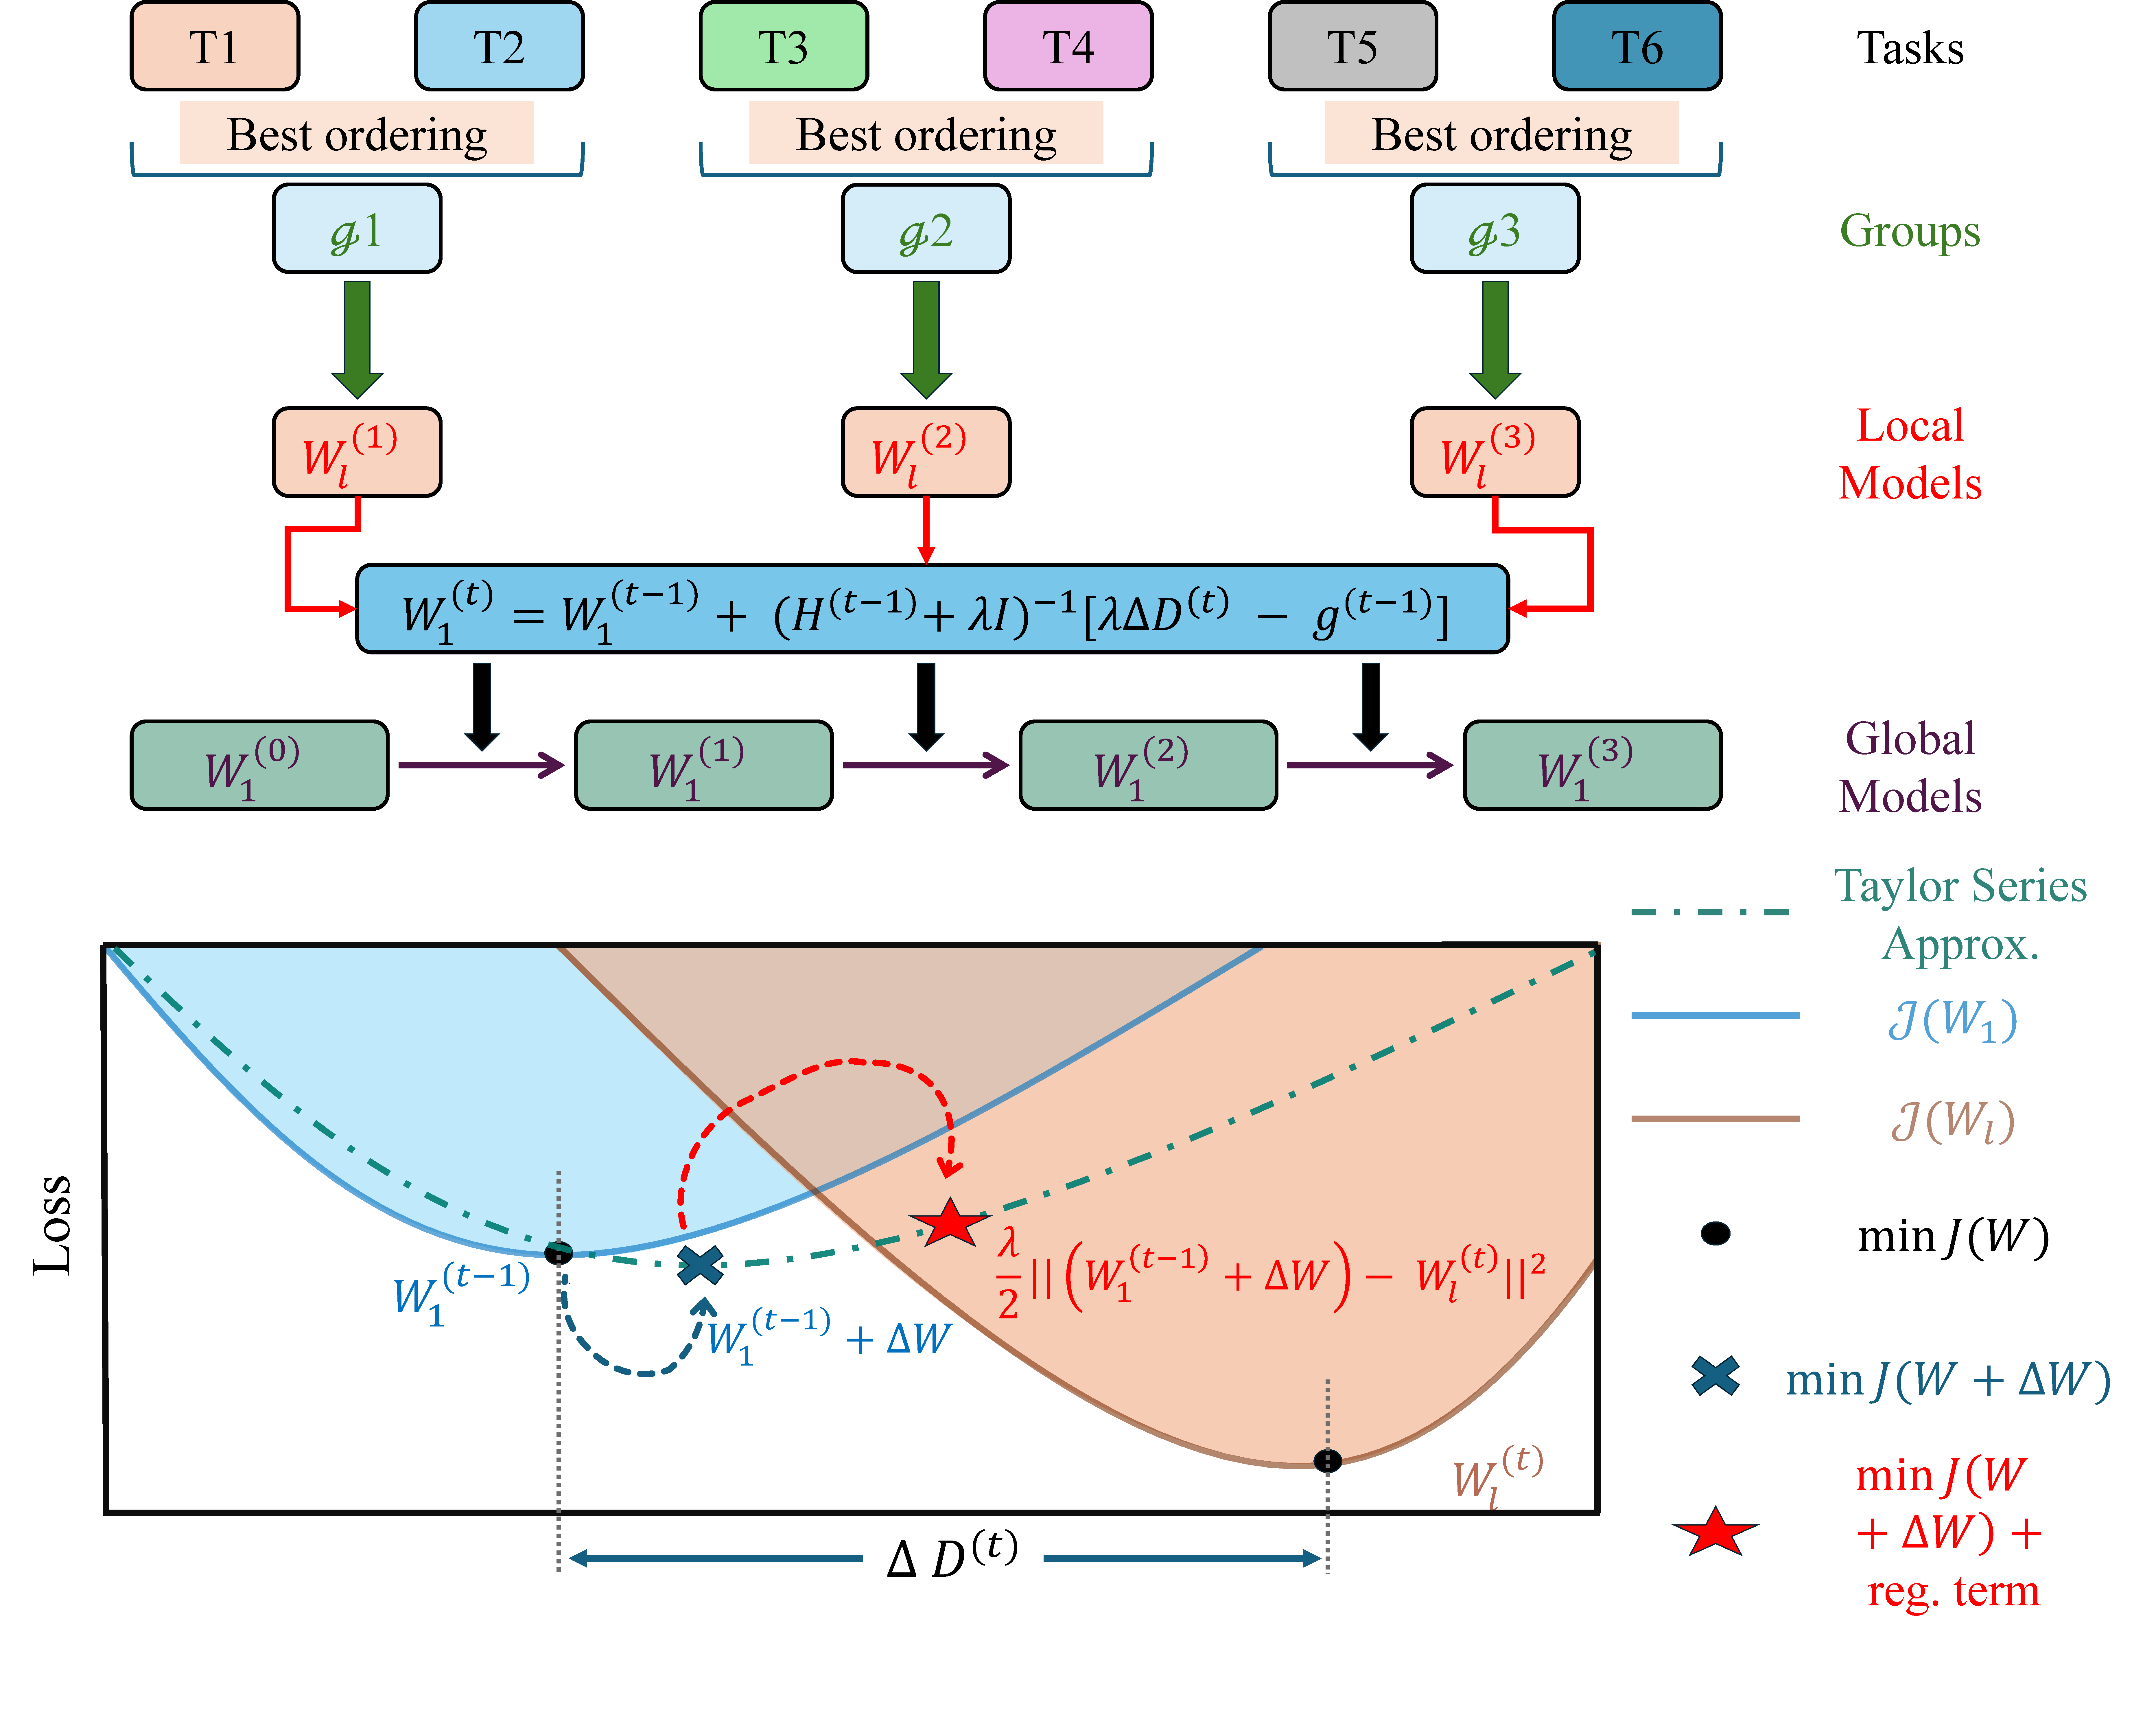
\includegraphics[width=\columnwidth]{figures/exp.pdf}
  \caption{(top)~The HTCL framework for a sequence of six tasks partitioned into three groups ($\G_1, \G_2, \G_3$). Within each group, all $\gsize!$ (here $2!$) intra-group permutations are evaluated through neural network training to provide $\wlT{1}, \wlT{2}, \wlT{3}.$ These three results are successively integrated into the hierarchical model $\whT{1}{t}$. (bottom)~Illustration of the update rule on a loss landscape. The current hierarchical model $\whT{1}{t-1}$ (blue) integrates knowledge from the local model $\wlT{t}$ (brown). Rather than naively minimizing $\J(\w)$, HTCL approximates $\J(\whT{1}{t-1}+\Dw)$ (blue cross) using a second-order Taylor expansion of the loss around $\whT{1}{t-1}$ with a regularization term that penalizes deviation from $\wlT{t}$. 
    This yields the updated hierarchical model $\whT{1}{t}$ (red star).}
    \label{fig:htcl-overview}
\end{figure}

Each hierarchical level progressively smooths and consolidates information from the faster layers below it. Lower levels (smaller $i$) retain adaptability to recent tasks, while higher levels (larger $i$) maintain long-term stability through slower updates. Empirically, we find that deeper hierarchies (e.g., $\nlev=3$) provide improved resistance to catastrophic forgetting, particularly in long task sequences. Quantitative results and ablation studies are provided in Section~\ref{sec:results}. Beyond the empirical evidence, two theoretical results underpin HTCL's design. Theorem~\ref{thm:perf-bound-main} establishes an accuracy floor relative to random task ordering, and Proposition~\ref{thm:tradeoff-main} formalizes the trade-off between permutation-search cost and marginal accuracy gain as a function of group size $k$. 

\begin{theorem}[Performance bound]
\label{thm:perf-bound-main}
HTCL's performance is never worse, in expectation, than encountering tasks in a uniformly random order. The best intra-group permutation selected within each group provides a guaranteed accuracy floor that random arrival cannot beat in expectation, and typically yields strictly better performance. Full statement and proof in Appendix~\ref{app:performance-bounds}.
\end{theorem}

\begin{proposition}[Complexity--performance trade-off] 
\label{thm:tradeoff-main}
The cost of intra-group permutation search grows linearly with the group size $\gsize$, while the marginal accuracy gain decays factorially. Most of the available improvement is therefore captured at small group sizes ($\gsize{=}2$ or $\gsize{=}3$), and larger groups buy negligible accuracy at substantial computational cost. Full derivation and assumptions in Appendix~\ref{app:proof_tradeoff}; Appendix~\ref{app:break-even-point} empirically confirms the break-even at $\gsize{=}3$ on SplitMNIST.
\end{proposition}

\begin{remark}[Time and space complexity]
\label{rem:complexity}
The exact curvature-aware update in \eqref{eq:hier_update-main} requires forming and inverting a $\pdim \times \pdim$ Hessian, resulting in worst-case time $\Theta(\pdim^3)$ and memory $\Theta(\pdim^2)$ (or $\Theta(\nlev \pdim^3)$ and $\Theta(\nlev \pdim^2)$ for an $\nlev$-level hierarchy). In practice, HTCL employs scalable second-order approximations (e.g., diagonal Hessian approximation and group size $\gsize < 5$) which reduce both time and memory to near-linear. Complete derivations and comparisons with other CL methods are provided in Appendix~\ref{app:complexity}.
\end{remark}
\section{Experiments}
\label{sec:results}

We evaluated HTCL on (i) three image classification benchmarks: SplitMNIST~\cite{lecun2002gradient} (10 classes divided into 5 tasks, 2 classes per task), Split CIFAR-100~\cite{krizhevsky2009learning} (100 classes divided into 10 tasks, 10 classes per task) and a 100-class subset of ImageNet~\cite{deng2009imagenet} (ImageNet-100, 10 tasks of 10 classes each); (ii) a graph node classification problem using the Split Cora dataset~\cite{mccallum2000automating}; and (iii) a text classification problem on 20 Newsgroups~\cite{lang1995newsweeder} dataset  to demonstrate HTCL's generality across domains. All experiments other than ImageNet-100 use the \textit{domain-incremental} learning setting. ImageNet-100 is evaluated under both \textit{domain-incremental} and \textit{class-incremental} protocols (see Appendix~\ref{app:large-scale}). All experiments are performed on an NVIDIA A100 GPU.

\begin{figure*}[!htbp]
    \centering
    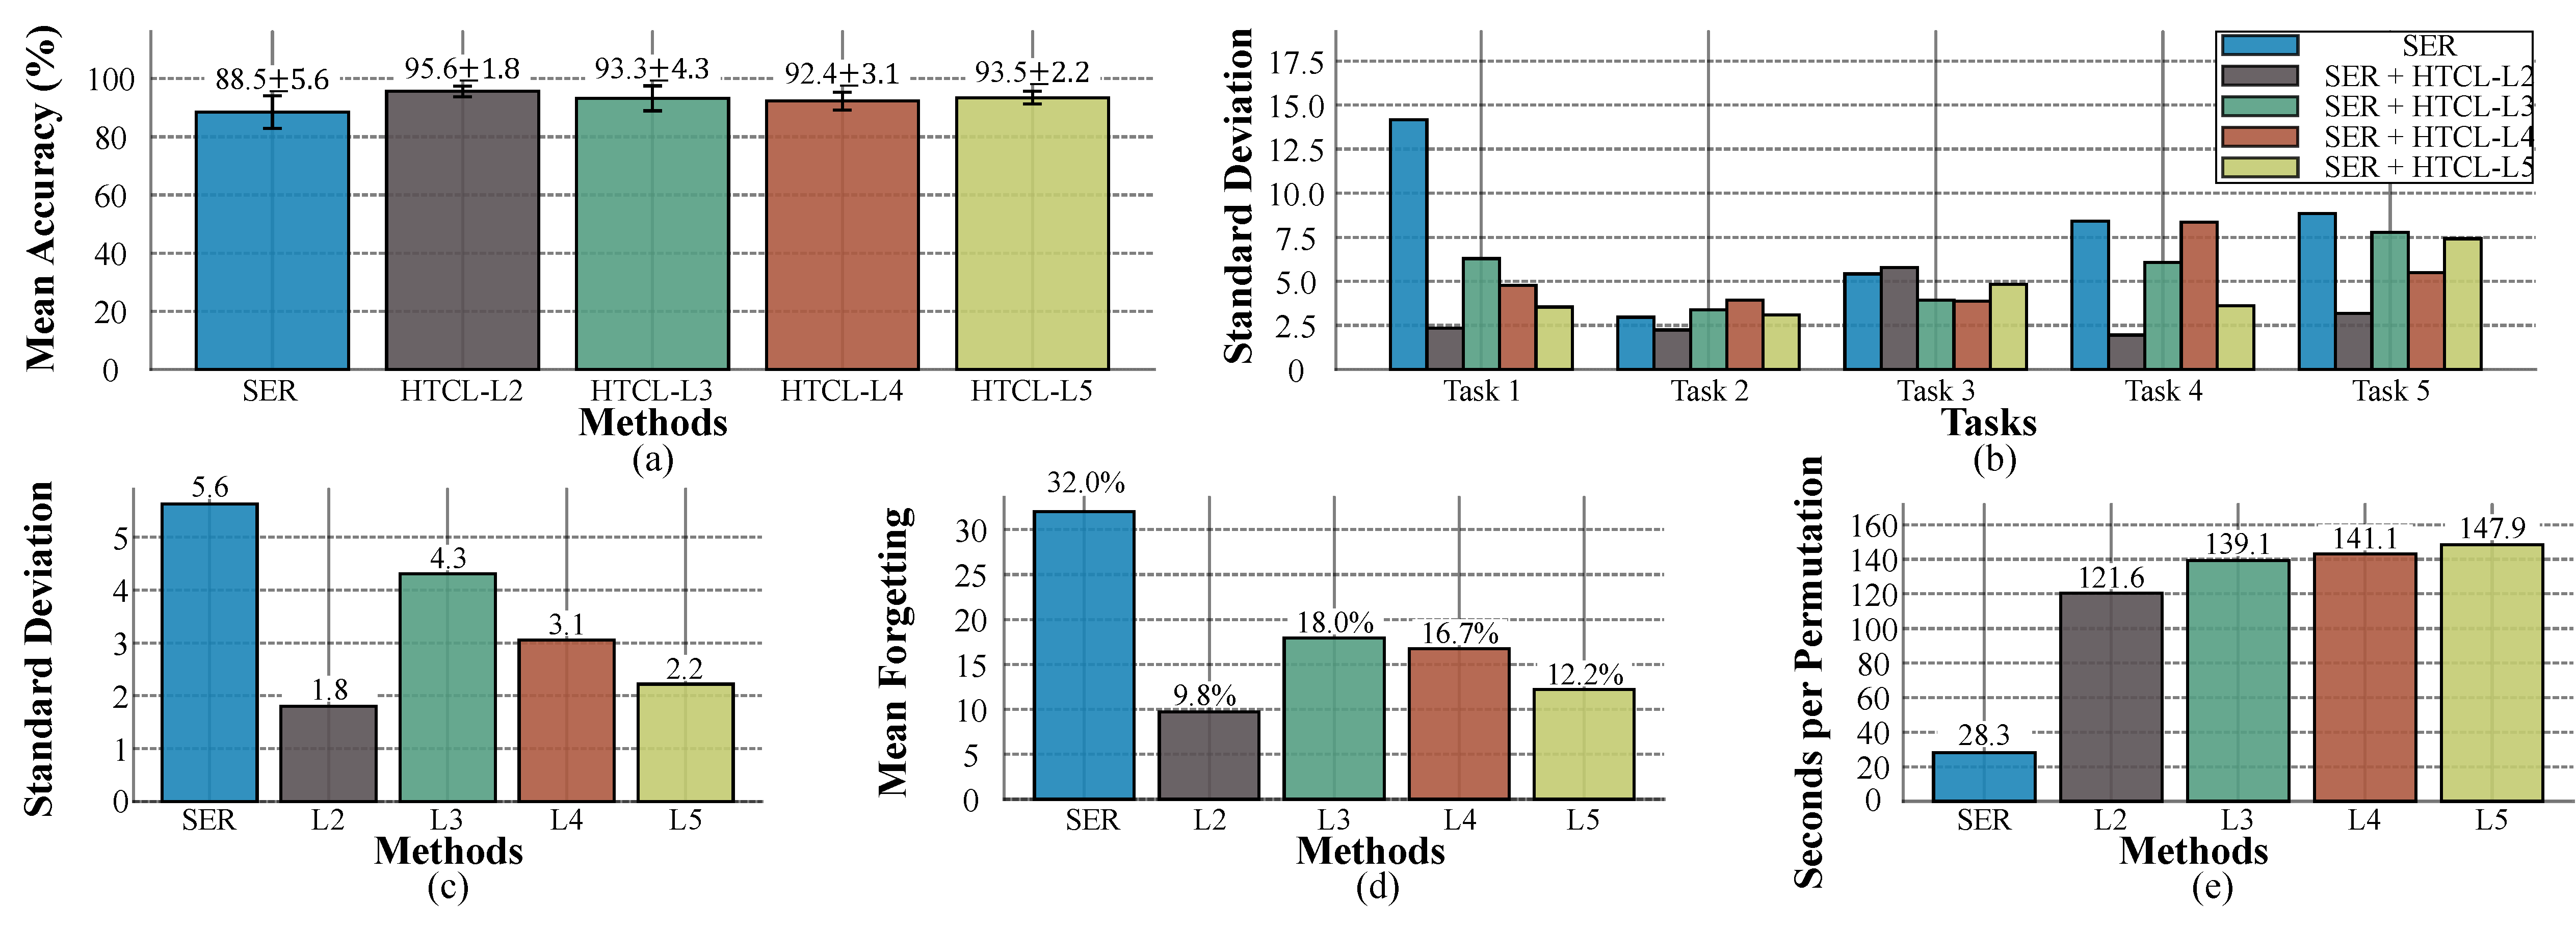
\includegraphics[width=0.90\textwidth, trim={0.3cm 0.3cm 0.3cm 0.3cm}, clip]{figures/updated_figures/ser.pdf}
    \caption{\textbf{Task-order robustness and memory retention of HTCL with SER on SplitMNIST.} 
    (a) Mean accuracy with standard-deviation error bars for SER and SER + HTCL-L\{2,3,4,5\}. 
    (b) Per-task standard deviation across permutations. 
    (c) Overall standard deviation. 
    (d) Mean forgetting. 
    (e) Wall-clock time per permutation. 
    HTCL reduces task-order variance and forgetting at moderate compute overhead.}
    \label{fig:ser-results}
\end{figure*}

\begin{figure}[!t]
  \centering
  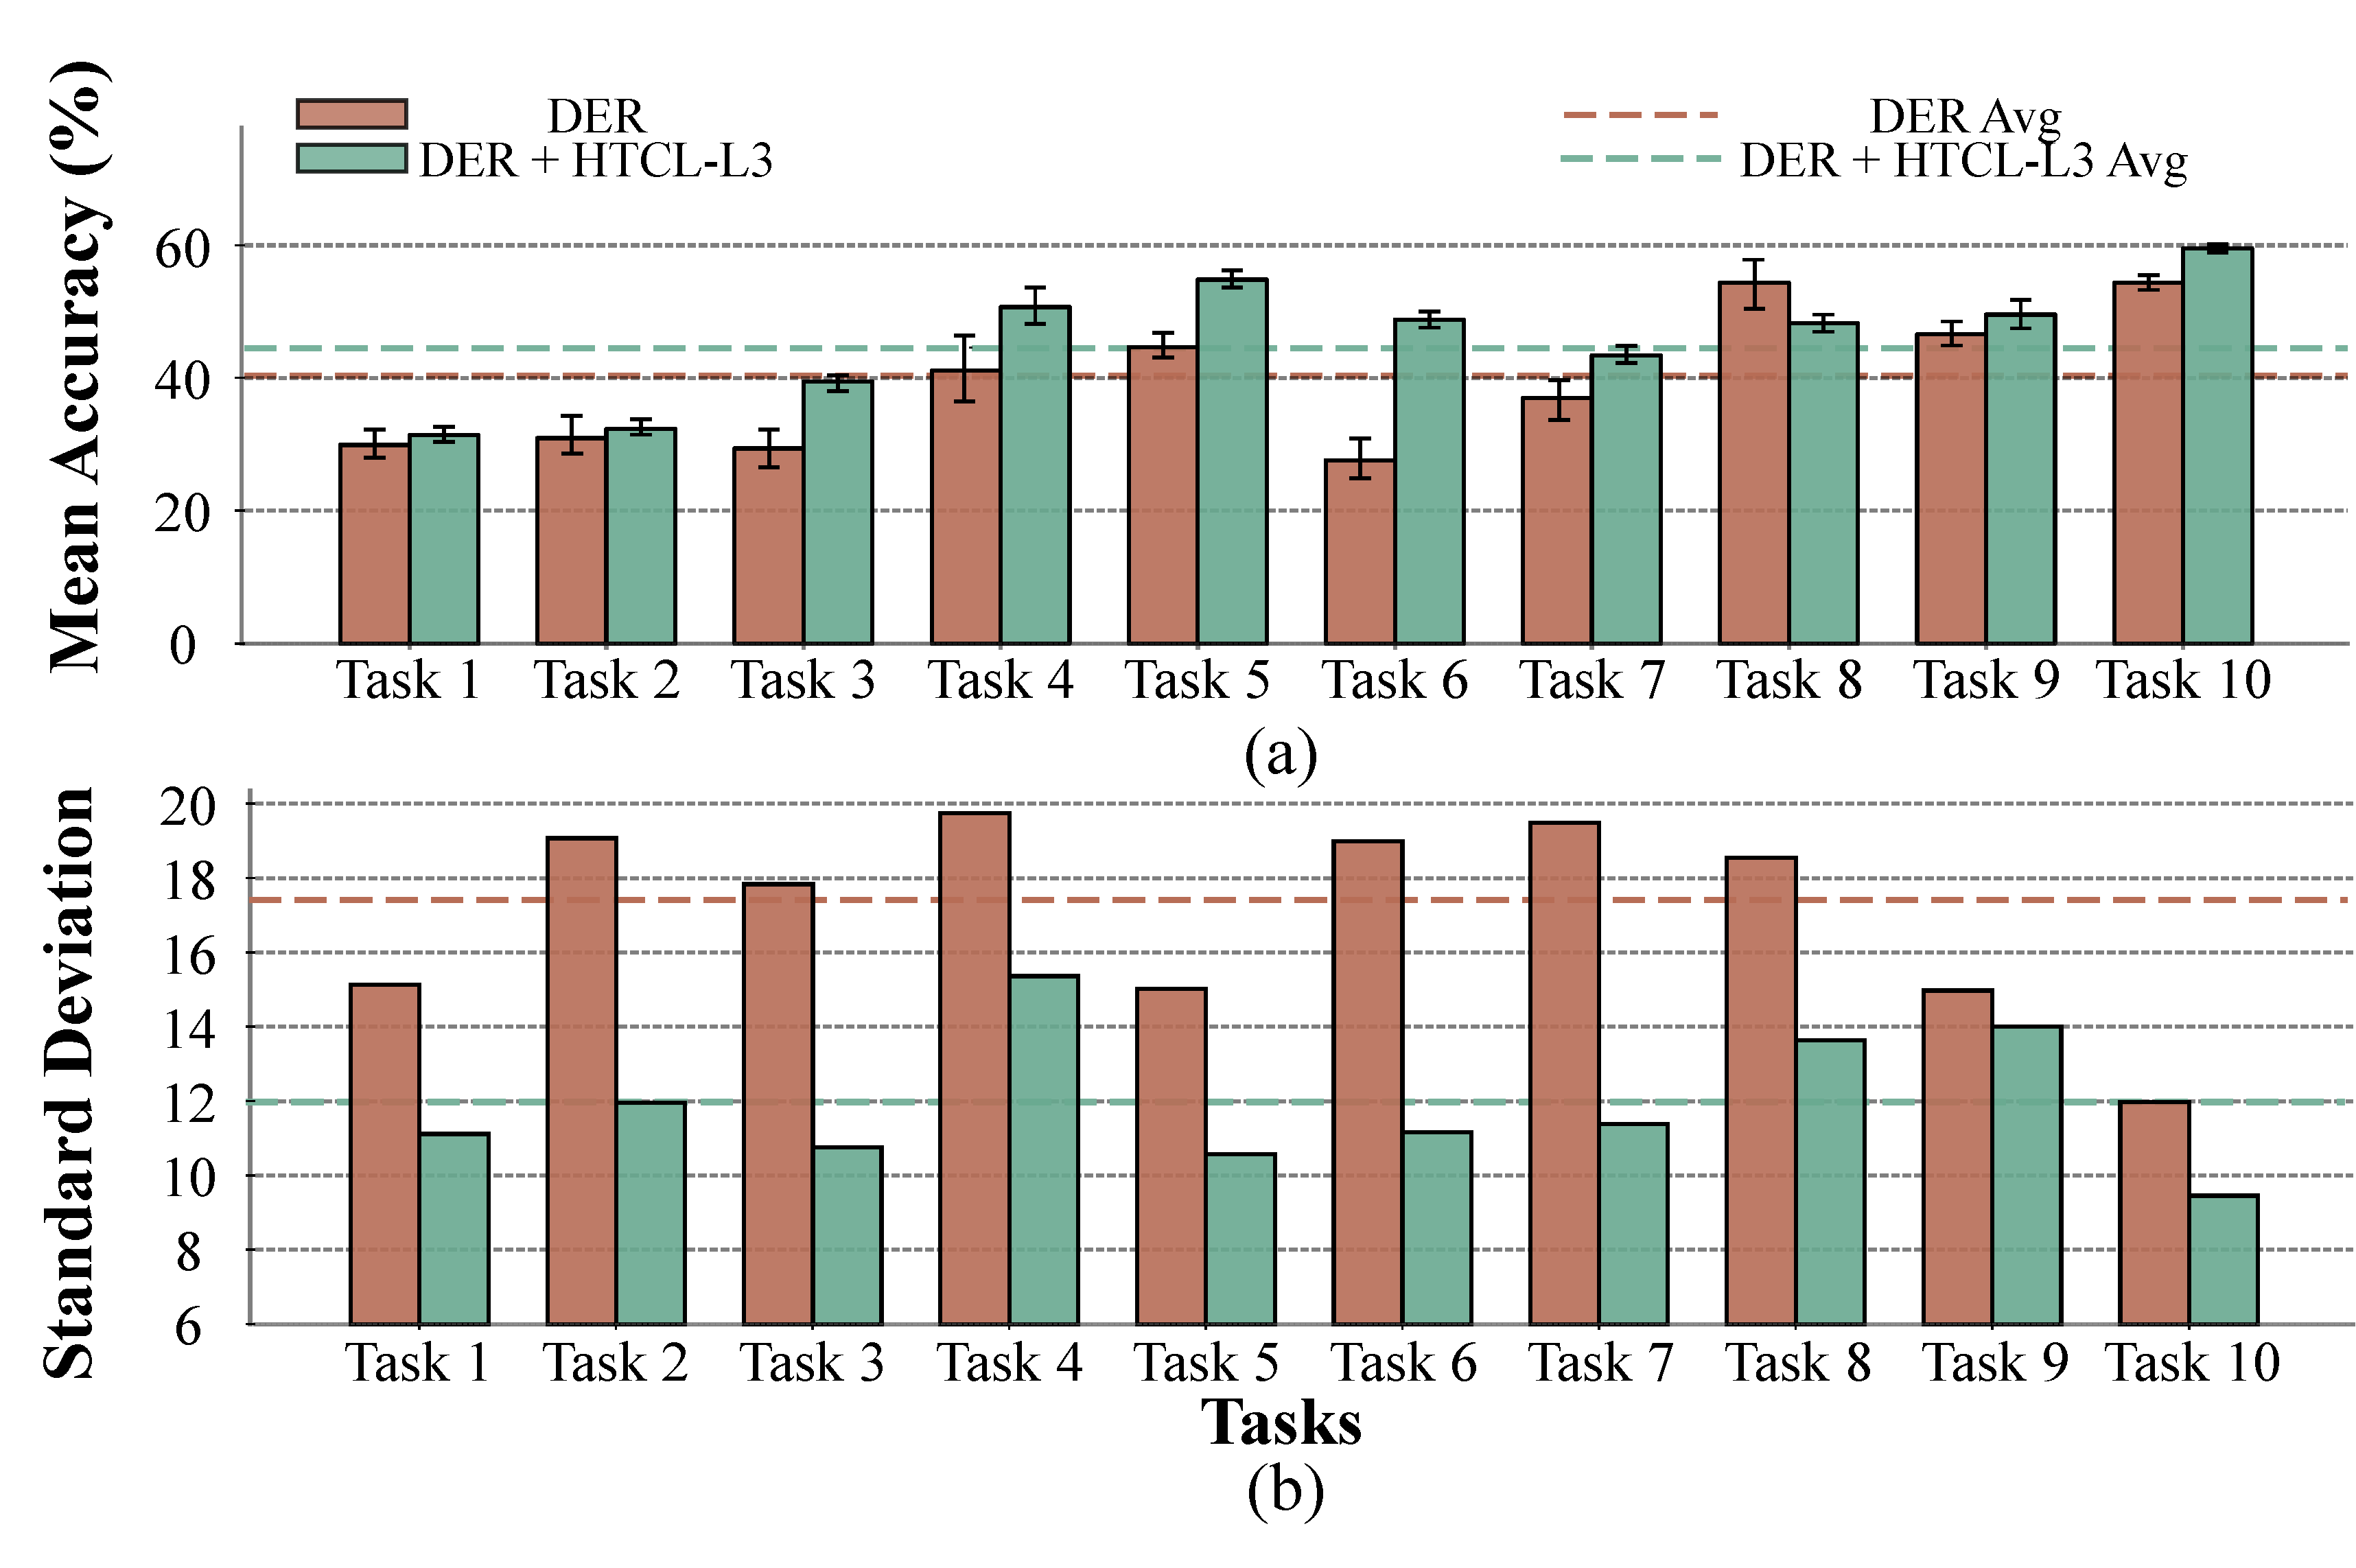
\includegraphics[width=\columnwidth]{figures/updated_figures/der.pdf}
  \caption{\textbf{Scalability of HTCL under long task sequences.} We extend the two-level local–global structure to a three-level hierarchy as described in Eq.~\eqref{eq:multi_hierarchy}, using DER as a baseline for illustration. The three-layer HTCL demonstrates higher memory retention and lower variance when handling long task sequences. (a) Mean accuracy per task: DER + HTCL-L3 achieves $45.2\%$ compared to $40.6\%$ for DER alone. (b) Standard deviation per task: DER + HTCL-L3 maintains a lower standard deviation ($12.0$) compared to DER alone ($17.4$).}
    \label{fig:extended}
\end{figure}

We compared the HTCL method against top seven baseline CL methods spanning replay-based, regularization-based, and hybrid approaches: Strong Experience Replay (SER)~\cite{zhuo2023continual}, Dark Experience Replay (DER)~\cite{buzzega2020dark}, Experience Replay (ER), DualNet~\cite{pham2021dualnet}, iCaRL~\cite{rebuffi2017icarl}, EWC~\cite{kirkpatrick2017overcoming}, and Spectral Regularizer (SR)~\cite{ICLR2025_5565ab68}. These baselines were selected to include methods with state-of-the-art performance on our benchmarks (SER), foundational approaches in CL (EWC, ER), and recently proposed techniques (SR). In our framework, each baseline trains the \textit{local} model, while the consolidated model is updated via the Taylor series–based rule in Eq.~\eqref{eq:hier_update-main}. We calculate \textit{average accuracy}, \textit{average forgetting} and \textit{standard deviation} of accuracy to demonstrate our results~\cite{lopez2017gradient, chaudhry2018efficient}. A detailed list of hyperparameters and other details on experimental setup can be found in Appendix~\ref{app:extended-results}.

We first present representative results illustrating the performance of HTCL on SplitMNIST (see Figure~\ref{fig:ser-results}) using SER as a baseline through mean accuracy, task-order sensitivity, forgetting, and computational overhead. Next, we demonstrate the scalability of our HTCL to extended task sequences using DER on Split CIFAR-100 (see Figure~\ref{fig:extended}). A comprehensive comparison against seven baseline models across four diverse datasets (SplitMNIST, Split CIFAR-100, Split Cora, 20 Newsgroups) can be found in Table~\ref{tab:mean-std}. We further investigate the effects of memory buffer size on HTCL performance in Appendix~\ref{app:small-buffer}. Finally, since our consolidation method resembles some similarities with federated aggregation, we present a comparative analysis against FedProx~\cite{li2020federated} and FedAvg~\cite{mcmahan2017communication} in Appendix~\ref{app:federated}.

\textbf{Enhanced task-order robustness.} Panels~(b) and~(c)  of Figure~\ref{fig:ser-results} characterize stability with respect to task-order permutations. Panel~(b) shows that HTCL enables lower per-task variance, with reductions of up to $82\%$ on the most volatile tasks (e.g., Task 1), suggesting that individual tasks are less sensitive to the order in which they are encountered. Panel~(c) summarizes this effect at the sequence level, where HTCL markedly reduces the overall standard deviation by $67.9\%$ (dropping from $5.6$ to $1.8$) across permutations, with HTCL-L2 exhibiting the strongest robustness. This stabilizing effect generalizes effectively to other modalities; on Cora (graph) and 20 Newsgroups (text), HTCL reduces standard deviation by approximately $38\%$ and $33\%$ respectively, confirming that the method's robustness is not limited to image domains (results are shown in Table~\ref{tab:mean-std}).

\textbf{Accuracy and memory retention.} Panel~(a) in Figure~\ref{fig:ser-results} shows that incorporating the Taylor-based consolidation consistently improves mean accuracy relative to the SER baseline, with HTCL-L2 achieving the largest gain of $7.1$ percentage points ($95.6\%$ vs $88.5\%$). We observe similar improvements in non-image tasks, where HTCL boosts mean accuracy by $5.8$ percentage points on Cora and $6.3$ percentage points on 20 Newsgroups. This improvement reflects stronger retention of earlier tasks rather than overfitting to the final task, a trend that is corroborated by the forgetting metric in Panel~(d), where HTCL-L2 exhibits a drastic drop in forgetting compared to the baseline ($9.8\%$ vs $32.0\%$). This $22.2\%$ reduction on SplitMNIST is mirrored in the graph and text domains, where forgetting drops by over $10$ percentage points relative to the baseline. These results indicate that the global consolidation step effectively preserves previously learned representations, preventing the catastrophic overwriting of weights associated with earlier tasks. Together, these results demonstrate that the observed accuracy gains stem principally from improved long-term memory retention.

\begin{figure*}[!t]
    \centering
    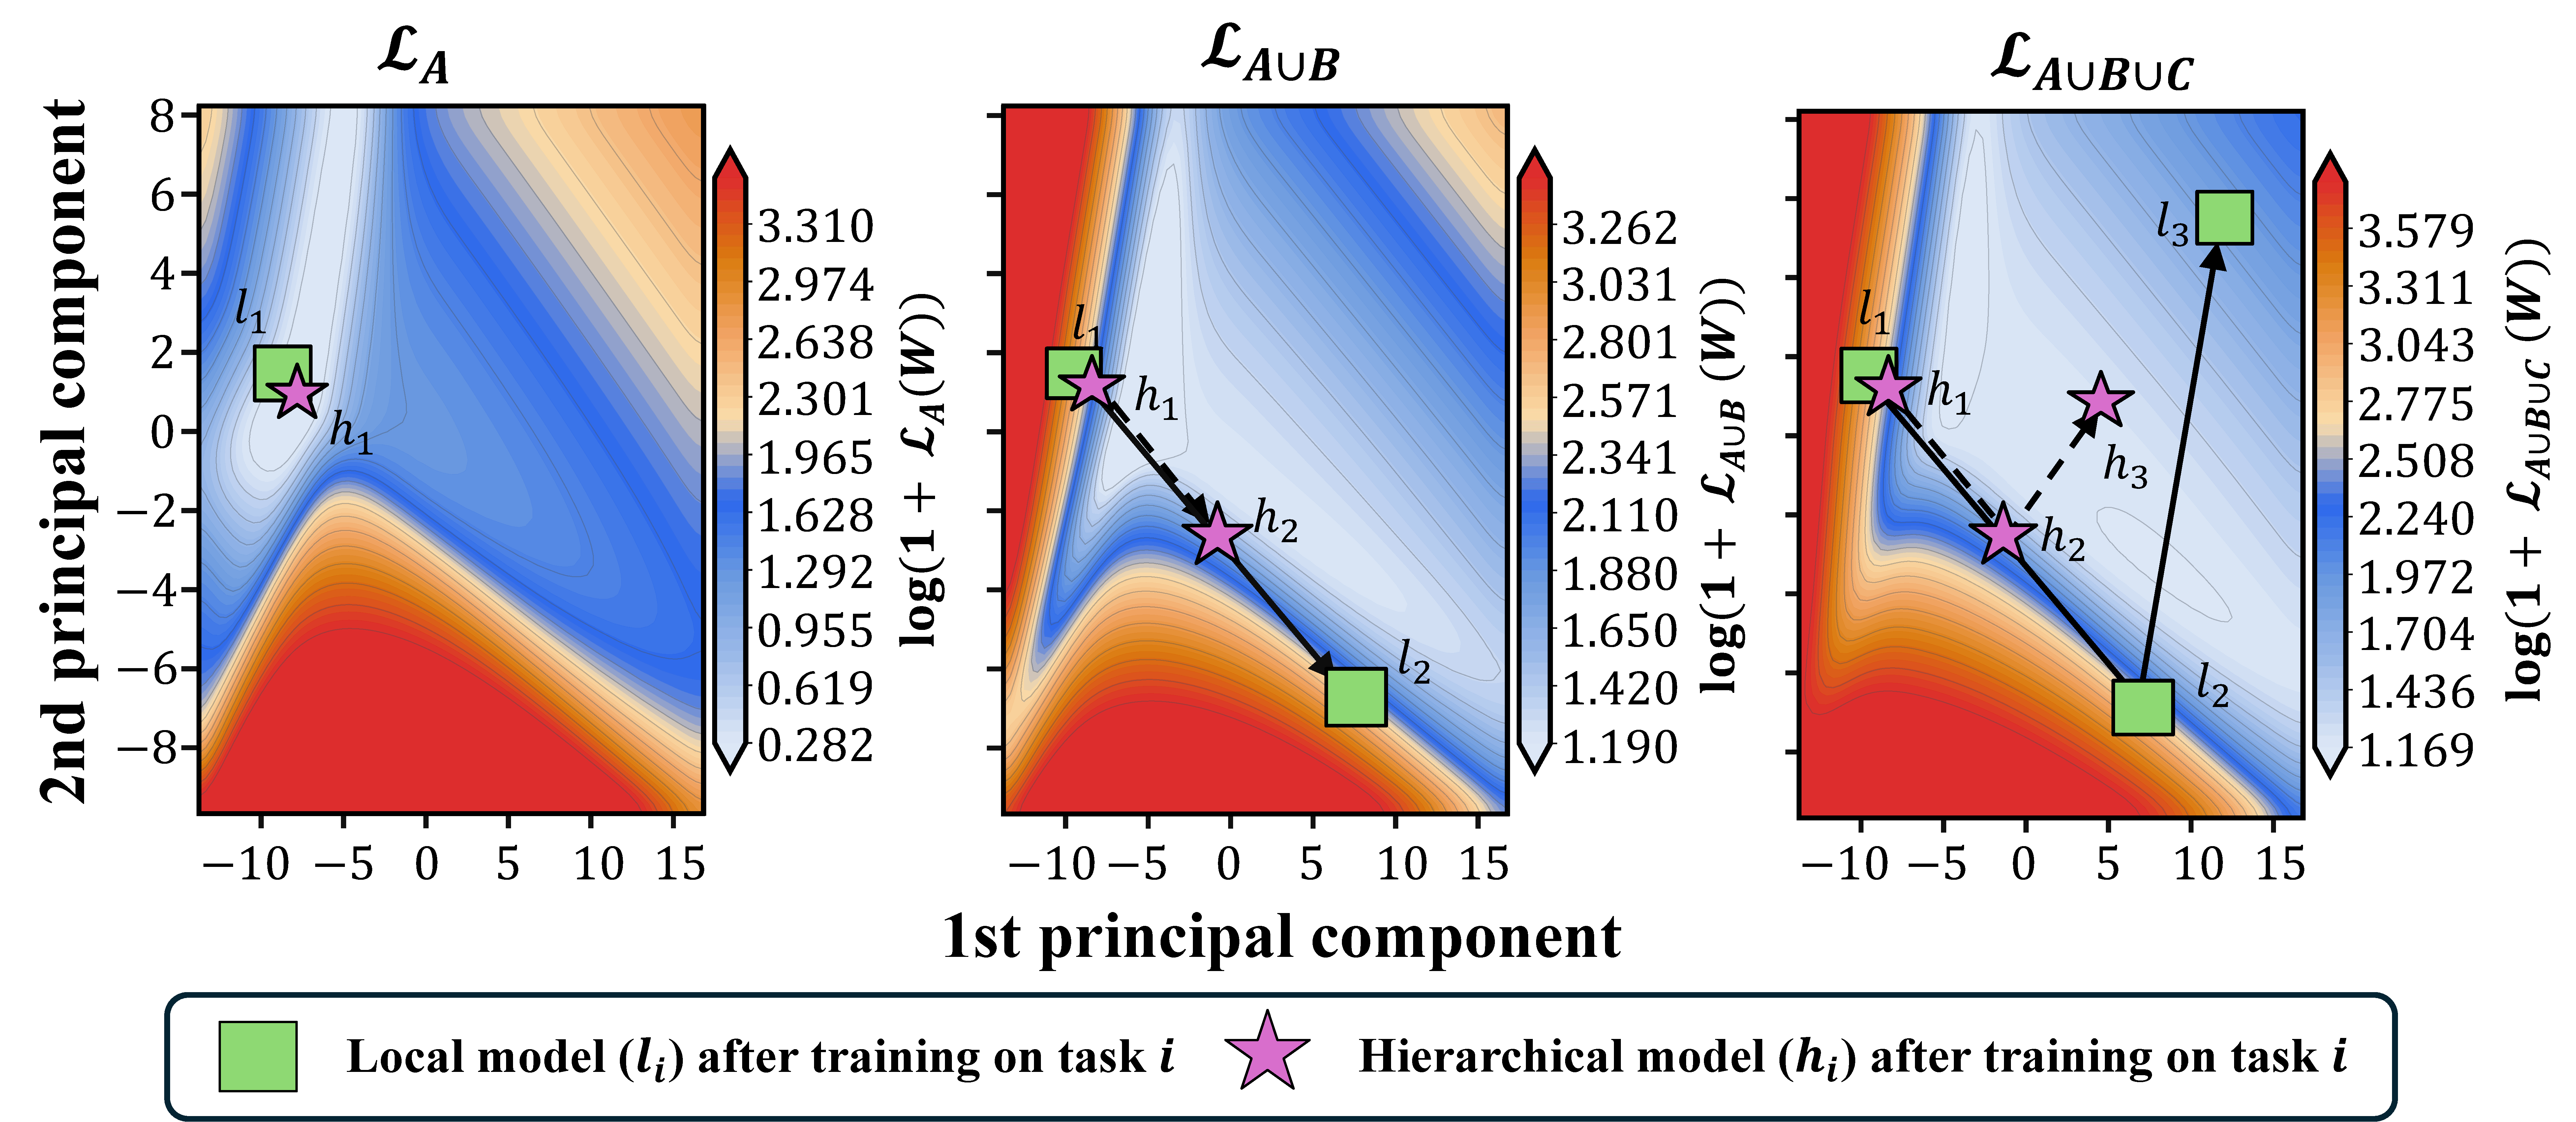
\includegraphics[width=0.8\textwidth]{figures/loss_landscape/loss_landscape.pdf}
    \caption{\textbf{Loss-landscape geometry of HTCL across a SplitMNIST class-incremental sequence.} Green squares mark local models $\ell_i$ adapted to task $i$; pink stars mark hierarchical models $h_i$ after Taylor consolidation. Across panels, the local trajectory drifts toward task-specific minima along ridges of the cumulative loss, while the hierarchical trajectory remains within the shared low-loss corridor of $\mathcal{L}_{A \cup B \cup C}$.}
    \label{fig:loss_landscape}
\end{figure*}

\begin{table*}[!htbp]
\centering
\caption{Final accuracy and variability across domains under the domain-incremental setting using a replay buffer of 50 samples for SplitMNIST, Cora, and 20 Newsgroups, and 500 samples for CIFAR-100. Mean accuracy, standard deviation, and mean forgetting are computed over 120 task-order permutations for SplitMNIST and 20 Newsgroups, 6 permutations for Cora, and 200 random permutations for CIFAR-100. Across all methods, incorporating HTCL consistently reduces task-order sensitivity, yielding substantially lower standard deviations while preserving or improving mean accuracy. $\uparrow$ denotes an increase and $\downarrow$ denotes a decrease relative to the baseline. Best results within each method group are shown in \textbf{bold}.}
\label{tab:mean-std}
\resizebox{\textwidth}{!}{%
\begin{tabular}{lcccccccccccc}
\hline
\multirow{2}{*}{\textbf{Method}} &
  \multicolumn{12}{c}{\textbf{Datasets}} \\ \cline{2-13} 
 &
  \multicolumn{3}{c}{\textbf{SplitMNIST}} &
  \multicolumn{3}{c}{\textbf{CIFAR-100}} & 
  \multicolumn{3}{c}{\textbf{Cora}} & 
  \multicolumn{3}{c}{\textbf{20 Newsgroups}} \\ \hline
 &
  \textbf{Mean Acc.} &
  \textbf{Std} &
  \textbf{Mean Forget} &
  \textbf{Mean Acc.} &
  \textbf{Std} &
  \textbf{Mean Forget} &
  \textbf{Mean Acc.} &
  \textbf{Std} &
  \textbf{Mean Forget} &
  \textbf{Mean Acc.} &
  \textbf{Std} &
  \textbf{Mean Forget} \\ \hline
SER &
  88.5 & 5.6 & 32.0 &
  42.6 & 18.7 & 56.5 &
  72.5 & 6.8 & 28.5 &
  58.2 & 8.4 & 35.2 \\
SER + HTCL-L2 &
  \textbf{95.6}$\uparrow$ & \textbf{1.8}$\downarrow$ & \textbf{9.8}$\downarrow$ &
  44.7$\uparrow$ & 14.9$\downarrow$ & 40.0$\downarrow$ &
  \textbf{78.3}$\uparrow$ & \textbf{4.2}$\downarrow$ & \textbf{18.2}$\downarrow$ &
  \textbf{64.5}$\uparrow$ & \textbf{5.6}$\downarrow$ & \textbf{24.8}$\downarrow$ \\
SER + HTCL-L3 &
  93.3$\uparrow$ & 4.3$\downarrow$ & 18.0$\downarrow$ &
  \textbf{46.2}$\uparrow$ & \textbf{12.5}$\downarrow$ & \textbf{30.0}$\downarrow$ &
  76.8$\uparrow$ & 5.1$\downarrow$ & 21.4$\downarrow$ &
  62.8$\uparrow$ & 6.3$\downarrow$ & 27.5$\downarrow$ \\ \hline
DER &
  86.5 & 4.9 & 35.0 &
  40.6 & 17.4 & 58.2 &
  70.2 & 7.2 & 30.8 &
  55.8 & 9.1 & 38.4 \\
DER + HTCL-L2 &
  \textbf{95.1}$\uparrow$ & \textbf{1.8}$\downarrow$ & \textbf{10.2}$\downarrow$ &
  43.0$\uparrow$ & 14.4$\downarrow$ & 42.6$\downarrow$ &
  \textbf{77.5}$\uparrow$ & \textbf{4.5}$\downarrow$ & \textbf{19.5}$\downarrow$ &
  \textbf{62.3}$\uparrow$ & \textbf{6.0}$\downarrow$ & \textbf{26.5}$\downarrow$ \\
DER + HTCL-L3 &
  92.3$\uparrow$ & 4.3$\downarrow$ & 18.8$\downarrow$ &
  \textbf{45.2}$\uparrow$ & \textbf{12.0}$\downarrow$ & \textbf{33.0}$\downarrow$ &
  75.2$\uparrow$ & 5.4$\downarrow$ & 22.8$\downarrow$ &
  60.5$\uparrow$ & 6.8$\downarrow$ & 29.2$\downarrow$ \\ \hline
ER &
  89.3 & 5.5 & 30.3 &
  38.0 & 20.0 & 60.0 &
  68.5 & 7.8 & 32.5 &
  54.4 & 9.8 & 42.0 \\
ER + HTCL-L2 &
  \textbf{92.0}$\uparrow$ & \textbf{3.5}$\downarrow$ & \textbf{12.5}$\downarrow$ &
  41.0$\uparrow$ & 17.0$\downarrow$ & 48.0$\downarrow$ &
  \textbf{74.2}$\uparrow$ & \textbf{5.2}$\downarrow$ & \textbf{22.0}$\downarrow$ &
  \textbf{58.5}$\uparrow$ & \textbf{6.8}$\downarrow$ & \textbf{32.5}$\downarrow$ \\
ER + HTCL-L3 &
  91.5$\uparrow$ & 4.0$\downarrow$ & 14.0$\downarrow$ &
  \textbf{43.5}$\uparrow$ & \textbf{15.5}$\downarrow$ & \textbf{40.0}$\downarrow$ &
  73.0$\uparrow$ & 5.8$\downarrow$ & 24.5$\downarrow$ &
  57.2$\uparrow$ & 7.4$\downarrow$ & 34.0$\downarrow$ \\ \hline
iCaRL &
  93.2 & 4.8 & 12.5 &
  41.8 & 17.2 & 54.4 &
  74.8 & 6.2 & 22.5 &
  60.5 & 7.5 & 30.2 \\
iCaRL + HTCL-L2 &
  \textbf{96.1}$\uparrow$ & \textbf{2.1}$\downarrow$ & \textbf{6.8}$\downarrow$ &
  44.2$\uparrow$ & 14.0$\downarrow$ & 42.5$\downarrow$ &
  \textbf{78.2}$\uparrow$ & \textbf{3.8}$\downarrow$ & \textbf{15.8}$\downarrow$ &
  \textbf{65.8}$\uparrow$ & \textbf{5.0}$\downarrow$ & \textbf{22.5}$\downarrow$ \\
iCaRL + HTCL-L3 &
  95.0$\uparrow$ & 3.4$\downarrow$ & 9.2$\downarrow$ &
  \textbf{46.6}$\uparrow$ & \textbf{11.8}$\downarrow$ & \textbf{35.0}$\downarrow$ &
  77.5$\uparrow$ & 4.5$\downarrow$ & 18.2$\downarrow$ &
  64.0$\uparrow$ & 5.8$\downarrow$ & 25.0$\downarrow$ \\ \hline
DualNet &
  89.2 & 9.0 & 15.0 &
  40.6 & 17.5 & 57.0 &
  71.8 & 8.5 & 26.2 &
  56.5 & 10.2 & 33.5 \\
DualNet + HTCL-L2 &
  90.5$\uparrow$ & 6.0$\downarrow$ & 10.5$\downarrow$ &
  41.5$\uparrow$ & 14.4$\downarrow$ & 45.0$\downarrow$ &
  75.5$\uparrow$ & 5.8$\downarrow$ & 19.0$\downarrow$ &
  61.2$\uparrow$ & 7.2$\downarrow$ & 26.8$\downarrow$ \\
DualNet + HTCL-L3 &
  \textbf{91.0}$\uparrow$ & \textbf{5.5}$\downarrow$ & \textbf{9.0}$\downarrow$ &
  \textbf{44.0}$\uparrow$ & \textbf{12.0}$\downarrow$ & \textbf{36.0}$\downarrow$ &
  \textbf{76.8}$\uparrow$ & \textbf{5.2}$\downarrow$ & \textbf{17.5}$\downarrow$ &
  \textbf{62.5}$\uparrow$ & \textbf{6.5}$\downarrow$ & \textbf{24.5}$\downarrow$ \\ \hline
SR &
  88.0 & 7.5 & 31.0 &
  13.0 & 24.0 & 65.0 &
  69.5 & 8.8 & 35.0 &
  54.2 & 10.5 & 40.5 \\
SR + HTCL-L2 &
  90.0$\uparrow$ & 5.0$\downarrow$ & 14.0$\downarrow$ &
  18.5$\uparrow$ & 20.0$\downarrow$ & 55.0$\downarrow$ &
  74.0$\uparrow$ & 6.0$\downarrow$ & 25.5$\downarrow$ &
  59.6$\uparrow$ & 7.5$\downarrow$ & 32.7$\downarrow$ \\
SR + HTCL-L3 &
  \textbf{91.0}$\uparrow$ & \textbf{4.0}$\downarrow$ & \textbf{12.0}$\downarrow$ &
  \textbf{22.0}$\uparrow$ & \textbf{18.0}$\downarrow$ & \textbf{48.0}$\downarrow$ &
  \textbf{75.5}$\uparrow$ & \textbf{5.2}$\downarrow$ & \textbf{22.0}$\downarrow$ &
  \textbf{61.0}$\uparrow$ & \textbf{6.8}$\downarrow$ & \textbf{29.1}$\downarrow$ \\ \hline
EWC &
  79.3 & 9.8 & 42.8 &
  12.5 & 23.5 & 68.0 &
  65.2 & 9.7 & 38.2 &
  48.5 & 11.1 & 45.8 \\
EWC + HTCL-L2 &
  85.2$\uparrow$ & 6.2$\downarrow$ & 28.9$\downarrow$ &
  16.8$\uparrow$ & 19.5$\downarrow$ & 58.0$\downarrow$ &
  70.9$\uparrow$ & 6.5$\downarrow$ & 28.6$\downarrow$ &
  54.7$\uparrow$ & 8.8$\downarrow$ & 35.5$\downarrow$ \\
EWC + HTCL-L3 &
  \textbf{87.0}$\uparrow$ & \textbf{5.0}$\downarrow$ & \textbf{24.0}$\downarrow$ &
  \textbf{19.3}$\uparrow$ & \textbf{17.1}$\downarrow$ & \textbf{52.5}$\downarrow$ &
  \textbf{72.5}$\uparrow$ & \textbf{5.8}$\downarrow$ & \textbf{25.5}$\downarrow$ &
  \textbf{56.0}$\uparrow$ & \textbf{7.2}$\downarrow$ & \textbf{33.3}$\downarrow$ \\ \hline
\end{tabular}%
}
\end{table*}

\textbf{Practical computational overhead.} Panel~(e) reports the computation time per permutation. HTCL introduces additional cost, increasing the time per permutation from $28.3$ seconds (SER) to $121.6$ seconds (HTCL-L2). However, this overhead scales gradually with hierarchy depth. In practice, this trade-off is highly favorable: while computational cost increases by approximately $4\times$, it yields a $69\%$ relative reduction in forgetting ($32.0\%$ to $9.8\%$) and a $68\%$ reduction in task-order variance ($5.6$ to $1.8$). This makes the method practical for CL scenarios where reliability and robustness to random task order are priorities over raw training speed.

\textbf{Generalization across methods.} Table~\ref{tab:mean-std} reports mean accuracy, standard deviation, and mean forgetting across multiple CL baselines under the domain-incremental setting. Across all baseline methods, incorporating HTCL consistently reduces standard deviation, demonstrating improved task-order robustness. For the strongest baselines such as SER and DER, HTCL also yields substantial gains in mean accuracy and reductions in forgetting, confirming that the Taylor-based consolidation rule is broadly complementary to existing approaches. The consistent reduction in standard deviation across all methods highlights HTCL's role as a variance-reducing mechanism that stabilizes learning regardless of the underlying baseline.  

\textbf{Scaling to modern transformer architectures.} To verify that HTCL transfers beyond convolutional baselines, we evaluate on a $100$-class ImageNet subset with a ViT-S/16 backbone ($\approx 21.7$M parameters) under both domain- and class-incremental protocols, using $k = 2$, $\nlev = 2$, and $200$ task permutations per setting. As reported in Appendix~\ref{app:large-scale} (Table~\ref{tab:imagenet100}), HTCL-L2 improves mean accuracy by $4.7$ to $8.1$ percentage points across five baselines while reducing both the standard deviation and forgetting in every configuration. The class-incremental setting is uniformly harder than the domain-incremental one, but the relative benefit of curvature-aware consolidation is preserved.

\textbf{Scaling to long task sequences.} {We extend the two-level framework to a three-level hierarchy via Eq.~\ref{eq:multi_hierarchy} and evaluate on Split CIFAR-100 with DER as the base method. The intermediate level adds a consolidation stage between the fast local and slow hierarchical models, progressively smoothing the updates across timescales. Figure~\ref{fig:extended} shows DER + HTCL-L3 reaching $45.2\%$ mean accuracy against $40.6\%$ for DER (panel a), with per-task standard deviation dropping from $17.4$ to $12.0$, over a $30\%$ reduction (panel b). HTCL-L3 also outperforms HTCL-L2 on CIFAR-100 (Table~\ref{tab:mean-std}) and prevents the sharp mid-sequence accuracy drops on Tasks 3--7 visible in the baseline. These results confirm that deeper hierarchies provide tangible benefits for extended task sequences, where the accumulated interference across many tasks overwhelms single-model learners. By distributing consolidation across multiple temporal scales, HTCL maintains stability without sacrificing the plasticity needed to learn new tasks.

\textbf{Loss-landscape geometry:} {To visualize how HTCL's update navigates the cumulative loss surface, we follow the two-dimensional loss-landscape protocol of
\cite{li2018visualizing} and generate Fig.~\ref{fig:loss_landscape}. The experiment is class-incremental on MNIST, with the ten digits partitioned into three sequential tasks $A = \{0, 1, 2\}$, $B = \{3, 4, 5\}$, and $C = \{6, 7, 8, 9\}$, learned by a small MLP under HTCL with a group size $k = 3$. The six weight vectors produced over the three consolidation steps (the three local snapshots $\ell_1, \ell_2, \ell_3$ and the three hierarchical snapshots $h_1, h_2, h_3$) are projected onto the plane spanned by the first two principal components of their joint trajectory. On this fixed plane we render three panels, one per step, by sweeping a $75 \times 75$ grid, evaluating the cross-entropy loss at every grid point on the cumulative task set seen so far, and plotting $\log(1 + \mathcal{L}_{\cdot}(\mathbf{w}))$.


\section{Conclusion}\label{sec:conclusion}

In this work, we propose an alternative approach to mitigating task-order sensitivity in CL without depending on exhaustive combinatorial search over task permutations. Our framework decouples the learning process into local exploration for identifying the best intra-group performances and a hierarchical consolidation mechanism that integrates these localized solutions to achieve global robustness to task order. By combining hierarchical structure with second-order updates, HTCL enables a principled strategy of knowledge consolidation across multiple timescales. We believe that this perspective provides a practical path toward scalable continual learners that remain reliable under long task horizons while being compatible with existing CL methods. 

\appendices


\section{Related Works}\label{app:related_work}

\textbf{Paradigms in CL.}
In recent years, interest in CL has risen, especially from the deep learning research community~\cite{achille2018life, nguyen2017variational, schwarz2018progress, tasnim2024recast}. CL approaches are generally categorized into three paradigms: \emph{regularization-based}, \emph{replay-based}, and \emph{architecture-based} methods \cite{parisi2019continual,nguyen2019toward,schwarz2018progress}.

Regularization-based methods constrain parameter updates to protect prior knowledge. \emph{Elastic Weight Consolidation} (EWC) \cite{kirkpatrick2017overcoming} and \emph{Synaptic Intelligence} (SI) \cite{zenke2017continual} penalize deviation from parameters important to previous tasks. \emph{Online EWC} \cite{chaudhry2018efficient} and \emph{Stable SGD}~\cite{mirzadeh2020dropout} extend these ideas to continuous task streams and smoother optimization.

Replay-based methods alleviate forgetting by explicitly revisiting prior data or learned representations. \emph{Experience Replay} (ER), \emph{Strong ER (SER)}~\cite{zhuo2023continual}, and \emph{Dark ER (DER)}~\cite{buzzega2020dark} maintain small exemplar buffers, while \emph{Generative Replay} techniques \cite{shin2017continual,van2018generative} synthesize pseudo-samples from previous distributions. Exemplar-based systems such as \emph{iCaRL} \cite{rebuffi2017icarl} combine replay with incremental classifiers.

Architecture-based approaches \cite{fernando2017pathnet,masse2018alleviating,li2017learning} mitigate interference by expanding or routing subnetworks to isolate knowledge across tasks. Although effective in preventing forgetting, they typically incur high computational or memory costs and reduced scalability. Despite their progress, these paradigms collectively continue to struggle with the \emph{stability–plasticity dilemma}, particularly under extended task sequences and non-stationary environments \cite{chen2023stability,de2021continual}.

\textbf{Multi-Timescale and Dual-Model Approaches.}
Beyond these standard paradigms, some recent works employ multiple learners operating at different temporal scales. DualNet~\cite{pham2021dualnet}, for example, maintains a fast learner and a slow learner inspired by Complementary Learning Systems. Their fast model is trained using replayed examples, combining both raw buffer samples and latent features from the slow model. The slow learner is also updated through replay. Although this architecture resembles our use of local and hierarchical models, the mechanisms differ substantially. Unlike dual-model systems which rely on standard rehearsal, HTCL repurposes the replay buffer to approximate the curvature of the loss landscape (Hessian) for a regularization step, rather than for blind rehearsal. Consequently, the hierarchical models evolve solely through a Taylor series approximation of the loss, enabling principled multi-timescale integration. This distinction allows HTCL to function as a model-agnostic consolidation layer rather than a replay-driven dual-network system.

\textbf{Task Ordering and Sequence Sensitivity.}
Recent studies demonstrate that task order profoundly affects CL performance \cite{bell2022effect,riemer2018learning,yoon2019scalable}. Models trained on identical tasks but different sequences can yield widely varying accuracies due to path-dependent optimization. While curriculum learning leverages structured ordering to encourage transfer, standard CL frameworks generally assume fixed or random task orders, lacking robustness under arbitrary permutations. Efforts to address this include additive parameter decomposition for order invariance \cite{yoon2019scalable} and order-robust objectives or loss regularizers \cite{dohare2024loss,guo2024continual}. Nonetheless, the factorial complexity of possible permutations makes brute-force optimization infeasible \cite{knoblauch2020optimal}, leaving order sensitivity an open challenge.

\textbf{Relation to Federated Learning.}
Our hierarchical design shares superficial similarity with multi-model frameworks in \emph{Federated Learning} (FL) \cite{mcmahan2017communication,li2020federated}. In FL, distributed clients train local models whose updates are aggregated on a central server to preserve privacy and reduce communication cost. FedAvg~\cite{mcmahan2017communication} aggregates local models by simple parameter averaging, implicitly assuming that all local updates are equally compatible. FedProx~\cite{li2020federated} extends this approach by introducing a proximal term that constrains local updates to remain close to the global model, improving stability under heterogeneous client distributions. FedCurv~\cite{shoham2019overcoming} employs curvature-based regularization to further stabilize aggregation.

However, CL differs fundamentally  from FL. FL addresses spatial heterogeneity across distributed clients, whereas CL handles temporal distributional shifts within a single learner. The curvature-aware consolidation in HTCL is conceptually related to methods like FedCurv, but HTCL integrates information hierarchically over time rather than across parallel clients. \textbf{Detailed experimental comparisons with FL baselines can be found in Appendix~\ref{app:federated}}, confirming that HTCL outperforms both FedAvg and FedProx when applied to sequential task integration and highlighting the importance of consolidation mechanisms tailored to temporal learning.

\textbf{Summary and Distinction.}
In summary, prior methods have mitigated forgetting via replay, regularization, or network expansion, but they remain vulnerable to task-order bias and scalability challenges. Few works explicitly formalize order robustness. In contrast, \emph{HTCL} introduces a principled, multi-level Taylor series framework that unifies local adaptability and hierarchical stability, yielding order-invariant and scalable CL behavior.

\section{Consolidation Equation~\eqref{eq:hier_update-main}}
\label{app:update-proof}

\begin{theorem}
\label{prop:main}
If $\mathbf{H}^{(t-1)} + \reg \mathbf{I} \succ 0$, the minimizer of the surrogate objective \eqref{eq:surrogate} is:
\begin{equation}
\label{eq:deltaW}
\Dw^{*} = \left(\mathbf{H}^{(t-1)} + \reg \mathbf{I}\right)^{-1}\!\left(\reg \, \Dd^{(t)} - \mathbf{g}^{(t-1)}\right)
\end{equation}
and the updated hierarchical weights are:
\begin{equation}
\label{eq:hier_update}
\whT{1}{t} = \whT{1}{t-1} + \left(\mathbf{H}^{(t-1)} + \reg \mathbf{I}\right)^{-1}\!\left(\reg \, \Dd^{(t)} - \mathbf{g}^{(t-1)}\right)
\end{equation}
where $\Dd^{(t)} = \wlT{t} - \whT{1}{t-1}$. The surrogate is strictly convex and $\Dw^{*}$ is the global minimizer.
\end{theorem}

\begin{proof}

Taking the gradient of \eqref{eq:surrogate} with respect to $\Dw$ and setting it to zero:
\begin{align*}
    \nabla_{\Dw} &\Bigg[ \underbrace{\J(\whT{1}{t-1})}_{\text{const.}} + {\mathbf{g}^{(t-1)}}^\top \Dw + \tfrac{1}{2} \Dw^\top \mathbf{H}^{(t-1)} \Dw \\
    &\quad + \tfrac{\reg}{2} \left\| \Dw - \Dd^{(t)} \right\|^2 \Bigg] = 0 \\
    &\Rightarrow \mathbf{g}^{(t-1)} + \mathbf{H}^{(t-1)} \Dw + \reg \left(\Dw - \Dd^{(t)}\right) = 0 \\
    &\Rightarrow \left(\mathbf{H}^{(t-1)} + \reg \mathbf{I}\right) \Dw = \reg \, \Dd^{(t)} - \mathbf{g}^{(t-1)} 
\end{align*}

If the smallest eigenvalue of $\mathbf{H}^{(t-1)}$ is denoted by $\mu_{\min}(\mathbf{H}^{(t-1)})$, then the eigenvalues of $\mathbf{H}^{(t-1)} + \reg \mathbf{I}$ are shifted by $\reg$, giving
\begin{equation*}
    \mu_{\min}\left(\mathbf{H}^{(t-1)} + \reg \mathbf{I}\right) = \mu_{\min}\left(\mathbf{H}^{(t-1)}\right) + \reg.
\end{equation*}
Therefore, to guarantee positive definiteness, $\reg$ must satisfy
\begin{equation*}
    \reg > -\mu_{\min}\left(\mathbf{H}^{(t-1)}\right).
\end{equation*}
If this condition holds, then $\mathbf{H}^{(t-1)} + \reg \mathbf{I} \succ 0$ and is invertible, ensuring the surrogate is strictly convex with a global minimizer and we obtain the state solution. 
\end{proof}

\section{Recursive Formulation of the Global Update Rule}
\label{app:recursive}

The recursive formulation presented in Lemma~\ref{lem:recursive} generalizes the one-step Taylor series-based update in Eq.~\eqref{eq:hier_update} to a two-point approximation. While the main paper focuses on the standard one-point second-order expansion around $\whT{1}{t-1}$, it may be  useful to understand how the cumulative effect of successive Taylor updates can be expressed in closed form. In particular, combining the updates at timestep $t-1$ and $t$ yields a two-point approximation in which the global model integrates information from two consecutive local models. This recursive view does not change the algorithm but highlights how HTCL accumulates second-order information over time and makes the additive structure inherent to sequential Taylor series expansions. 

\begin{lemma}[Recursive formulation]
\label{lem:recursive}
Suppose the global updates at consecutive timesteps follow the Eq.~\eqref{eq:hier_update} and assume each matrix $\mathbf{H}^{(s-1)}+\reg \mathbf{I}$ is invertible. Then the cumulative second-order integration of local models into the global weights across the two timesteps yields
\begin{equation}
\label{eq:recursive}
\begin{aligned}
\whT{1}{t} 
&= \whT{1}{t-2} 
+ (\mathbf{H}^{(t-2)} + \reg \mathbf{I})^{-1}\!\big[\reg \Dd^{(t-1)} - \mathbf{g}^{(t-2)}\big] \\
&\qquad + (\mathbf{H}^{(t-1)} + \reg \mathbf{I})^{-1}\!\big[\reg \Dd^{(t)} - \mathbf{g}^{(t-1)}\big]
\end{aligned}
\end{equation}
\end{lemma}

\begin{proof}
Update at time $t-1$ using the update rule:
\[
\whT{1}{t-1} = \whT{1}{t-2} + (\mathbf{H}^{(t-2)}+\reg \mathbf{I})^{-1}\!\big[\reg \Dd^{(t-1)} - \mathbf{g}^{(t-2)}\big]
\]
Now write the update at time $t$:
\[
\whT{1}{t} = \whT{1}{t-1} + (\mathbf{H}^{(t-1)}+\reg \mathbf{I})^{-1}\!\big[\reg \Dd^{(t)} - \mathbf{g}^{(t-1)}\big]
\]
Substitute the expression for $\whT{1}{t-1}$ into the update at time $t$:
\[
\boxed{
\begin{aligned}
\whT{1}{t}
&= \whT{1}{t-2} + (\mathbf{H}^{(t-2)}+\reg \mathbf{I})^{-1}\!\big[\reg \Dd^{(t-1)} - \mathbf{g}^{(t-2)}\big] \\
&\qquad + (\mathbf{H}^{(t-1)}+\reg \mathbf{I})^{-1}\!\big[\reg \Dd^{(t)} - \mathbf{g}^{(t-1)}\big]
\end{aligned}
}
\]
Re-arranging terms yields the claimed identity \eqref{eq:recursive}. The derivation requires only linear algebraic substitution and the invertibility of the matrices $(\mathbf{H}^{(s-1)}+\reg \mathbf{I})$ to justify the closed-form updates. 
\end{proof}

\section{Performance Bounds for the Algorithm~\ref{alg:task-ordering}}
\label{app:performance-bounds}

\begin{theorem}[Performance Bound]
\label{prop:group_vs_random}
Let $\T$ be a set of $\ntasks$ tasks partitioned into $\ngroups$ disjoint groups $\G_1, \ldots, \G_\ngroups$, each of size $\gsize$ such that  $\ntasks \approx \ngroups \cdot \gsize$). %
For each group $\G_j$, let $\gpermset_j$ denote the set of its $k!$ intra-group permutations, where each $\sigma \in \gpermset_j$ specifies an ordering of tasks within $\G_j$. Let the average accuracy of group $\G_j$ achieved with permutation $\sigma$ after training the Neural Network be
$\Acc_j^{(\gperm)} = \frac{1}{\gsize} \sum_{\tsk \in \G_j} \Eval_{\tsk}\!\left(\w^{(j)}\right),$
where $\Eval_{\tsk}(\w^{(j)})$ represents performance measure on $\tsk$ for a given $\gperm$. %
    Then if each $\gperm_j$ is drawn uniformly at random from $\gpermset_j$,
    \[
    \sum_{j=1}^{\ngroups} \Acc^{\mathrm{HTCL}}(\G_j) \geq \E_{\gperm_1, \ldots, \gperm_\ngroups}\!\left[\sum_{j=1}^{\ngroups} \Acc_j^{(\gperm_j)}\right],
    \]
    where $A^{HTCL}(G_j)$ denotes the average accuracy of group $G_j$ achieved with the proposed HTCL approach.
\end{theorem}

\begin{proof}
For each group $\G_j$ and any chosen permutation $\gperm_j \in \gpermset_j$, the performance of the HTCL, by definition, satisfies
\[
\Acc^{\mathrm{HTCL}}(\G_j) = \max_{\gperm \in \gpermset_j} \Acc_j^{(\gperm)} \geq \Acc_j^{(\gperm_j)}
\]
Summing over all $\ngroups$ groups, we have
\[
\sum_{j=1}^{\ngroups} \Acc^{\mathrm{HTCL}}(\G_j) \geq \sum_{j=1}^{\ngroups} \Acc_j^{(\gperm_j)}
\]
This holds for any fixed choice of $(\gperm_1, \ldots, \gperm_\ngroups)$. Taking expectation over random selections $\gperm_j \sim \mathrm{Uniform}(\gpermset_j)$ preserves the inequality (since the left-hand side is deterministic). Hence, we obtain the following lower bound on the expected performance of HTCL
\[
\boxed{\sum_{j=1}^{\ngroups} \Acc^{\mathrm{HTCL}}(\G_j) \geq \E_{\gperm_1, \ldots, \gperm_\ngroups}\!\left[\sum_{j=1}^{\ngroups} \Acc_j^{(\gperm_j)}\right]}
\]

\end{proof}

\subsection{Proof of Complexity--Performance Trade-off}
\label{app:proof_tradeoff}

Theorem~\ref{prop:group_vs_random} establishes that HTCL achieves, at minimum, the expected performance under uniformly random intra-group orderings. We now quantify how this performance improves as a function of the group size $k$, and how it is traded-off against the factorial cost of intra-group permutation search.

Let $t$ tasks be partitioned into $m = \lceil t/k \rceil$ disjoint groups of size $k$. For each group $G_j$, HTCL evaluates all $k!$ intra-group permutations and selects the best-performing ordering. The cumulative performance is
\[
A_{\mathrm{HTCL}}(k) := \sum_{j=1}^{m} \max_{\sigma \in \varsigma_j} A_j^{(\sigma)}.
\]

The total number of permutations evaluated is
\begin{align}\label{eq:complexity}
C(k) = m \cdot k! \approx t \cdot (k-1)!,
\end{align}
while the full permutation space has size $|\Pi(t)| = t!$. The fraction of explored permutations is therefore
\[
\rho(k) := \frac{C(k)}{t!} = \frac{(k-1)!}{(t-1)!}.
\]

Let $A_{\mathrm{HTCL}}(t)$ denote the performance under full permutation coverage (i.e., a single group of size $t$ resulting in the best order of all the tasks), and define the performance gap
\[
\Delta_A(k) := A_{\mathrm{HTCL}}(t) - A_{\mathrm{HTCL}}(k),
\]
with worst-case gap $\Delta_{A,\max} := \Delta_A(1)$.

\emph{Assumption (i): Monotonicity.} The set of reachable task orderings under HTCL expands with $k$, hence $A_{\mathrm{HTCL}}(k)$ is non-decreasing and $\Delta_A(k) \ge 0$.

\emph{Remark.} For small $k$, HTCL only explores permutations that respect group boundaries. For example, with $t=4$ and $k=2$, the partition $\{1,2\}\{3,4\}$ cannot realize orderings such as $(2,3,1,4)$, since task $3$ cannot appear before completing the first group. When $k=4$, all $4!$ permutations become reachable. Thus, the set of explored permutations strictly enlarges with $k$, and taking a maximum over a larger set cannot decrease performance.

\medskip

\emph{Assumption (ii): Linear coverage model.} The residual performance gap, $\Delta_A(k)$, scales proportionally with the unexplored fraction of the permutation space ($1-\rho(k)$). In other words, we can define the performance gap as
\[
\Delta_A(k) = \mathcal{C} \Delta_{A,\max} \cdot (1 - \rho(k)),
\]
where $\mathcal{C}>0$ is a proportionality constant.

\emph{Remark.} This assumption models the unexplored permutations as contributing uniformly, in expectation, to the remaining gap. %

\begin{proposition}[Complexity--performance trade-off]
    Under the Assumptions $(i)$ and $(ii)$, we have the following relations to hold.

\[
\frac{C(k+1)}{C(k)} = k,
\]
\[
\Delta_A(k) - \Delta_A(k+1) \le \mathcal{C} \Delta_{A,\max} \cdot \frac{(k-1)(k-1)!}{(t-1)!}.
\]
\end{proposition}

\paragraph{Proof.}
The complexity follows directly from \eqref{eq:complexity}. %
\[
\frac{C(k+1)}{C(k)} = \frac{t \cdot k!}{t \cdot (k-1)!} = k.
\]

For the marginal improvement,
\[
\Delta_A(k) - \Delta_A(k+1)
= \mathcal{C} \Delta_{A,\max} \big(\rho(k+1) - \rho(k)\big).
\]
Using $\rho(k)=\frac{(k-1)!}{(t-1)!}$,
\[
\rho(k+1) - \rho(k)
= \frac{k! - (k-1)!}{(t-1)!}
= \frac{(k-1)(k-1)!}{(t-1)!},
\]
which yields the stated bound. \hfill $\square$

\emph{Remark.}
The computational cost grows linearly in $k$ (through the multiplicative factor $k$), while the corresponding improvement in performance is governed by a factorially small term for $k \ll t$. Consequently, most of the recoverable performance gain lies near full permutation coverage, and increasing $k$ yields diminishing returns beyond a small threshold. This explains the empirical saturation observed at small group sizes (e.g., $k \in \{2,3\}$), where HTCL captures a substantial portion of the achievable gain with modest computational overhead.

\section{Time and Space Complexity Analysis}
\label{app:complexity}

This appendix provides the detailed derivations supporting Remark~\ref{rem:complexity}.  
We analyze the exact and practical computational complexity of HTCL, including permutation search, 
curvature computation, and hierarchical integration, and compare these with  
standard single-model continual learning approaches.

\subsection{Exact Complexity of the Global Integration}

Recall that the global update for a single level is
\[
\whT{1}{t} 
= \whT{1}{t-1} 
+ (\mathbf{H}^{(t-1)} + \reg \mathbf{I})^{-1}\!\big[\reg(\wlT{t} - \whT{1}{t-1}) - \mathbf{g}^{(t-1)}\big].
\]

\begin{proposition}[Exact computational cost]
Forming and inverting the dense Hessian $\mathbf{H}^{(t-1)}\in\R^{\pdim\times \pdim}$ yields:
\[
\text{Time}_{\mathrm{exact}} = \Theta(\pdim^3), 
\qquad
\text{Memory}_{\mathrm{exact}} = \Theta(\pdim^2).
\]
\end{proposition}

\begin{proof}[Proof sketch]
A full Hessian contains $\pdim^2$ entries and computing all second derivatives requires  
$\Theta(\pdim^2)$ memory and up to $\Theta(\pdim^2 \!\cdot\! \text{samples})$ time.  
Solving $(\mathbf{H}+\reg \mathbf{I})x=b$ via dense Cholesky or Gaussian elimination requires  
$\Theta(\pdim^3)$ time.  
\end{proof}

\begin{corollary}[Hierarchy cost]
For an $\nlev$-level hierarchy:
\[
\text{Time}_{\mathrm{exact}}^{(\nlev)} = \Theta(\nlev \pdim^3),
\qquad 
\text{Memory}_{\mathrm{exact}}^{(\nlev)} = \Theta(\nlev \pdim^2).
\]
\end{corollary}

\subsection{Practical Complexity via Standard Approximations}

In practice, HTCL uses scalable second-order approximations, which reduce the cubic  
cost of exact Hessian inversion to near-linear time and memory.

\paragraph{Diagonal / Fisher approximation.}  
In our experiments we used this approximation. This approach stores only the diagonal of $\mathbf{H}$ or the Fisher information:
\[
\text{Time}_{\mathrm{diag}}=\Theta(\pdim),
\qquad 
\text{Memory}_{\mathrm{diag}}=\Theta(\pdim).
\]

\paragraph{Low-rank curvature approximation.}  
If $\mathbf{H}$ is approximated by a low-rank factorization of rank $r\ll \pdim$,  
then storing and applying the approximation requires:
\[
\text{Memory}_{\mathrm{low\text{-}rank}} = \Theta(r\pdim), 
\qquad
\text{Time}_{\mathrm{low\text{-}rank}} = \Theta(r\pdim).
\]

These are the two approximations used in our implementation.

\subsection{Cost of Permutation Search}

Let each task group contain $\gsize$ tasks.  
For each permutation $\perm\in \gpermset_\gsize$, the local model is trained for $N_{\text{iter}}$ minibatch updates, 
each costing $T_{\text{step}}$.  
Let $B$ denote the minibatch size.

\begin{proposition}[Exact permutation-search cost]
\[
\text{Time}_{\mathrm{perm,exact}}
= \gsize!\, N_{\text{iter}}\, T_{\text{step}}
= \Theta(\gsize!\, E \cdot \text{\#samples} \cdot \pdim).
\]
\end{proposition}

\begin{proof}[Proof sketch]
Each permutation requires $N_{\text{iter}}$ updates, each with forward--backward cost  
$T_{\text{step}} = \Theta(B\pdim)$.  
There are $\gsize!$ permutations.  
When models are evaluated sequentially, memory remains $\Theta(\pdim)$.  
\end{proof}

\paragraph{Practical setting.}  
We restrict the group size to $\gsize < 5$, so that  
\[
\gsize! \le 24
\]
is a small constant.  
Thus, the permutation-search overhead does not grow with the number of tasks and simplifies to:
\[
\text{Time}_{\mathrm{perm,practical}}
= \mathcal{O}(N_{\text{iter}}\,T_{\text{step}}),
\]
with no additional asymptotic dependence on $\gsize$.

\subsection{Total Practical Complexity of HTCL}

Combining bounded permutation search with curvature-regularized global integration gives:
\[
\boxed{
\begin{aligned}
\text{Time}_{\mathrm{HTCL}} 
={}&
\underbrace{\mathcal{O}(N_{\text{iter}}\,T_{\text{step}})}_{\text{permutation search } (\gsize! \le 24)} \\
&+
\underbrace{\mathcal{O}(\pdim)}_{\text{curvature update (diag or low-rank)}}
\end{aligned}
}
\]

\[
\boxed{
\text{Memory}_{\mathrm{HTCL}}
=
\Theta(\nlev \pdim)
+
\begin{cases}
\Theta(\pdim), & \text{(diagonal)},\\[3pt]
\Theta(r\pdim), & \text{(low-rank)}.
\end{cases}
}
\]

Typical configurations use  
$\gsize < 5$ (hence $\gsize!\le 24$),  
$r \ll \pdim$,  
and $\nlev \in \{2,3\}$,  
making HTCL comparable in cost to replay or EWC.

\subsection{Comparison with Standard Continual Learning Methods}

\paragraph{Regularization-based CL (EWC, SI, MAS).}  
Extra memory $\Theta(\pdim)$; extra per-step time $\Theta(\pdim)$. Lightweight but order-sensitive.

\paragraph{Replay-based CL (ER, DER, iCaRL).}  
Memory $\Theta(B_{\text{buf}}\cdot\text{sample size})$;  
extra time $\Theta(B_{\text{buf}}\cdot \pdim)$ due to rehearsal examples.

\paragraph{Architecture-based CL.}  
Memory grows with tasks: $\Theta(\sum_t \pdim_t)$;  
time increases with model expansion: $\Theta(\pdim_{\text{total}})$.

\paragraph{HTCL vs. standard CL.}  
HTCL trades moderate extra computation (bounded permutation search + curvature integration)  
for improved task-order robustness and multi-timescale consolidation, while maintaining  
near-linear practical complexity through diagonal or low-rank second-order approximations.

\section{Impact of Task Ordering on Model's Performance}
\label{app: task-order-impact}
In this section, we demonstrate the impact of task ordering on model performance across multiple domains, such as image classification, text classification, graph-based node classification, and synthetic sine regression tasks. Additionally, we examine the role of task order in facilitating positive transfer and mitigating interference.

\subsection{Illustrative Example: MNIST with BCL~\cite{raghavan2021formalizing}}
In this setup, a model sequentially learns five tasks in a BCL framework, each corresponding to different subsets of digits in the MNIST dataset. We analyze model performance under two distinct task sequences and log accuracy at each learning stage. Table~\ref{tab:mnist_results} presents task-wise accuracy values on corresponding test datasets for two task orders: Sequence A: $\langle 5, 1, 2, 3, 4 \rangle$ and Sequence B: $\langle1, 5, 2, 3, 4 \rangle$. 

\begin{table}[htbp]
\caption{Task order impact on MNIST with BCL. The table reports task-wise accuracy at each stage of training. Variability in final accuracy across task orders indicates sensitivity to task order.}
\label{tab:mnist_results}
\resizebox{\columnwidth}{!}{%
\begin{tabular}{cc|ccccc|c}
\textbf{} &
  \textbf{} &
  \multicolumn{5}{c|}{\textbf{Accuracy}} &
  \textbf{} \\ \hline
\rowcolor[HTML]{FFFFFF} 
\multicolumn{1}{c|}{\cellcolor[HTML]{FFFFFF}{\color[HTML]{000000} \textbf{Sequence}}} &
  {\color[HTML]{000000} \textbf{Learned Task}} &
  {\color[HTML]{000000} \textbf{Task\_1}} &
  {\color[HTML]{000000} \textbf{Task\_2}} &
  {\color[HTML]{000000} \textbf{Task\_3}} &
  {\color[HTML]{000000} \textbf{Task\_4}} &
  {\color[HTML]{000000} \textbf{Task\_5}} &
  {\color[HTML]{000000} \textbf{Average Accuracy}} \\ \hline
\rowcolor[HTML]{FFFFFF} 
\multicolumn{1}{c|}{\cellcolor[HTML]{FFFFFF}{\color[HTML]{000000} }} &
  {\color[HTML]{000000} 5} &
  {\color[HTML]{000000} 36.0} &
  {\color[HTML]{000000} 53.0} &
  {\color[HTML]{000000} 17.0} &
  {\color[HTML]{000000} 74.0} &
  {\color[HTML]{000000} 92.0} &
  {\color[HTML]{000000} 54.4} \\
\rowcolor[HTML]{FFFFFF} 
\multicolumn{1}{c|}{\cellcolor[HTML]{FFFFFF}{\color[HTML]{000000} }} &
  {\color[HTML]{000000} 1} &
  {\color[HTML]{000000} 100.0} &
  {\color[HTML]{000000} 53.0} &
  {\color[HTML]{000000} 17.0} &
  {\color[HTML]{000000} 79.0} &
  {\color[HTML]{000000} 87.0} &
  {\color[HTML]{000000} 67.2} \\
\rowcolor[HTML]{FFFFFF} 
\multicolumn{1}{c|}{\cellcolor[HTML]{FFFFFF}{\color[HTML]{000000} }} &
  {\color[HTML]{000000} 2} &
  {\color[HTML]{000000} 99.0} &
  {\color[HTML]{000000} 96.0} &
  {\color[HTML]{000000} 49.0} &
  {\color[HTML]{000000} 94.0} &
  {\color[HTML]{000000} 96.0} &
  {\color[HTML]{000000} 86.8} \\
\rowcolor[HTML]{FFFFFF} 
\multicolumn{1}{c|}{\cellcolor[HTML]{FFFFFF}{\color[HTML]{000000} }} &
  {\color[HTML]{000000} 3} &
  {\color[HTML]{000000} 96.0} &
  {\color[HTML]{000000} 90.0} &
  {\color[HTML]{000000} 93.0} &
  {\color[HTML]{000000} 87.0} &
  {\color[HTML]{000000} 89.0} &
  {\color[HTML]{000000} 91.0} \\
\rowcolor[HTML]{FFFFFF} 
\multicolumn{1}{c|}{\multirow{-5}{*}{\cellcolor[HTML]{FFFFFF}{\color[HTML]{000000} \textbf{A}}}} &
  {\color[HTML]{000000} \textbf{4}} &
  {\color[HTML]{000000} \textbf{97.0}} &
  {\color[HTML]{000000} \textbf{92.0}} &
  {\color[HTML]{000000} \textbf{88.0}} &
  {\color[HTML]{000000} \textbf{98.0}} &
  {\color[HTML]{000000} \textbf{95.0}} &
  {\color[HTML]{000000} \textbf{94.0}} \\ \hline
\rowcolor[HTML]{FFFFFF} 
\multicolumn{1}{c|}{\cellcolor[HTML]{FFFFFF}{\color[HTML]{000000} }} &
  {\color[HTML]{000000} 1} &
  {\color[HTML]{000000} 99.0} &
  {\color[HTML]{000000} 43.0} &
  {\color[HTML]{000000} 41.0} &
  {\color[HTML]{000000} 67.0} &
  {\color[HTML]{000000} 51.0} &
  {\color[HTML]{000000} 60.2} \\
\rowcolor[HTML]{FFFFFF} 
\multicolumn{1}{c|}{\cellcolor[HTML]{FFFFFF}{\color[HTML]{000000} }} &
  {\color[HTML]{000000} 5} &
  {\color[HTML]{000000} 98.0} &
  {\color[HTML]{000000} 53.0} &
  {\color[HTML]{000000} 11.0} &
  {\color[HTML]{000000} 75.0} &
  {\color[HTML]{000000} 94.0} &
  {\color[HTML]{000000} 66.2} \\
\rowcolor[HTML]{FFFFFF} 
\multicolumn{1}{c|}{\cellcolor[HTML]{FFFFFF}{\color[HTML]{000000} }} &
  {\color[HTML]{000000} 3} &
  {\color[HTML]{000000} 98.0} &
  {\color[HTML]{000000} 97.0} &
  {\color[HTML]{000000} 51.0} &
  {\color[HTML]{000000} 74.0} &
  {\color[HTML]{000000} 93.0} &
  {\color[HTML]{000000} 85.8} \\
\rowcolor[HTML]{FFFFFF} 
\multicolumn{1}{c|}{\cellcolor[HTML]{FFFFFF}{\color[HTML]{000000} }} &
  {\color[HTML]{000000} 3} &
  {\color[HTML]{000000} 96.0} &
  {\color[HTML]{000000} 95.0} &
  {\color[HTML]{000000} 94.0} &
  {\color[HTML]{000000} 63.0} &
  {\color[HTML]{000000} 45.0} &
  {\color[HTML]{000000} 78.6} \\
\rowcolor[HTML]{FFFFFF} 
\multicolumn{1}{c|}{\multirow{-5}{*}{\cellcolor[HTML]{FFFFFF}{\color[HTML]{000000} \textbf{B}}}} &
  {\color[HTML]{000000} \textbf{4}} &
  {\color[HTML]{000000} \textbf{92.0}} &
  {\color[HTML]{000000} \textbf{90.0}} &
  {\color[HTML]{000000} \textbf{86.0}} &
  {\color[HTML]{000000} \textbf{99.0}} &
  {\color[HTML]{000000} \textbf{91.0}} &
  {\color[HTML]{000000} \textbf{91.6}}
\end{tabular}%
}
\end{table}

To construct this table, we sequentially present tasks in a specified order, training the model on one task at a time. After training each task, we evaluate the model's performance on all tasks (previously seen or unseen) and record the accuracy. The accuracy values in the table represent the model's ability to retain knowledge as it progresses through the task sequence. The last column, labeled Average Accuracy, represents the model's overall performance across all tasks at each stage of training.

As training progresses, learning a new task typically leads to an immediate increase in accuracy for that specific task. However, previously learned tasks may experience either a stability effect (no change), positive transfer (accuracy improvement), or interference (accuracy degradation). The table reflects this effect, where the accuracy values evolve as more tasks are introduced. When the model completes training on Task 4, it has been exposed to all tasks, and its performance stabilizes across them. The lower half of the table follows the same calculation process for Sequence B, demonstrating how a different task order can result in varied accuracy trends. A comparison of task-wise accuracy and overall average accuracy between Sequence A and Sequence B clearly reveals variability in final performance, reinforcing the impact of task ordering on CL.

Since Task 4 appears at the end of both sequences, we expect its accuracy to be relatively high, as the model has just learned it. This is evident in rows 5 and 10 of Table~\ref{tab:mnist_results}. However, accuracy for other tasks varies significantly depending on their position in the sequence, demonstrating how order influences retention. Comparing Sequence A and Sequence B, we observe two key trends:

\begin{itemize}
    \item The accuracy of each task after it has been trained is shown in columns 3-7 and indicate a significant variation in accuracy~(approximately 2-5\%).
    \item The final average accuracy calculated after learning the final task differs between sequences (94\% and 91.6\%), suggesting that task order influences the performance.
\end{itemize}

This illustrative example demonstrates that task ordering affects both retention and adaptation. In subsequent sections, we extend this analysis across multiple datasets and learning paradigms.

\subsection{Impact of Task Number on Forgetting}
\label{app:impact-example}

\begin{figure}[htbp]
    \centering
    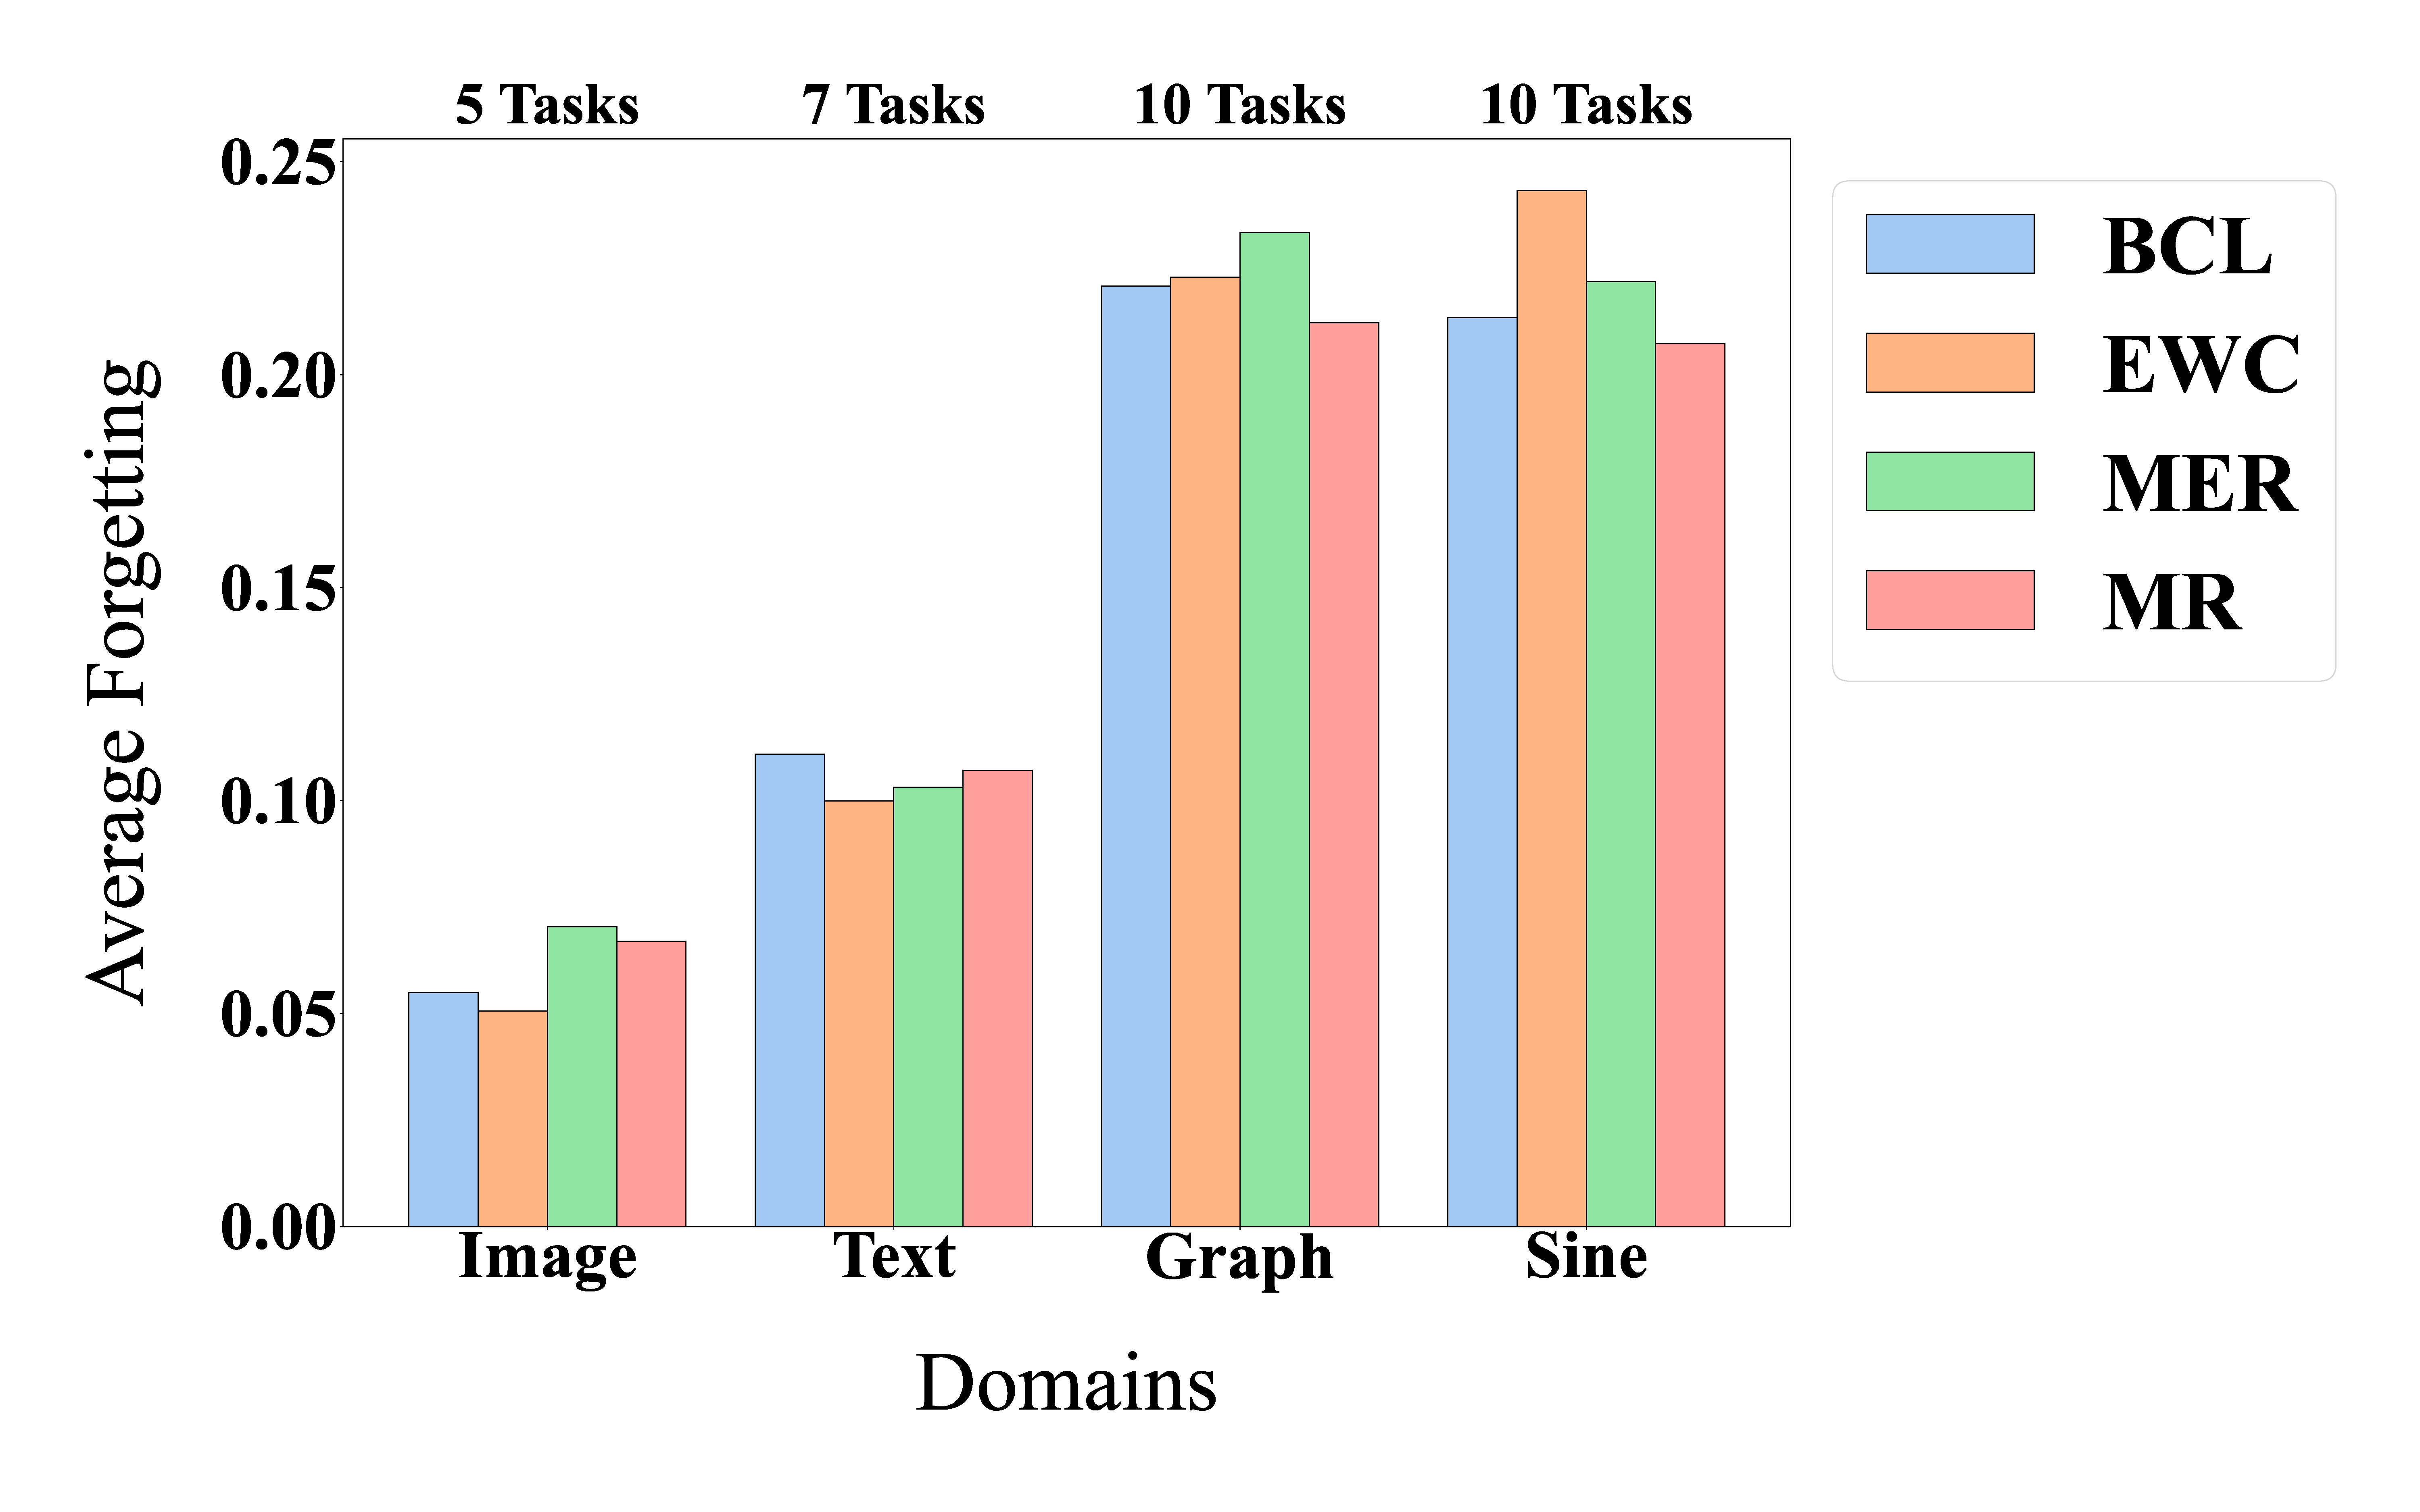
\includegraphics[width=\columnwidth]{figures/average_forgetting/average_forgetting_across_domains.pdf}
    \caption{Impact of the number of tasks on forgetting in CL across different domains. Forgetting increases as the number of tasks grows, with models experiencing up to 20\% accuracy drop in a 10-task setting.}
    \label{fig:forgetting_vs_tasks}
\end{figure}

Figure~\ref{fig:forgetting_vs_tasks} illustrates how forgetting exacerbates as the number of tasks increases. As we move left to right of the plot, the tasks increase. Corresponding to an increase in the number of tasks, the height of the bar plots~(which indicates the extent of forgetting) also increases. Moreover, this is true across multiple domains such as text, graph, image and numeric. This observation highlights the persistent challenge of knowledge retention in CL.

The trend depicted in Figure~\ref{fig:forgetting_vs_tasks} correlates with our hypothesis. That is, as the number of tasks increase, the likelihood of encountering suboptimal task sequences grows, leading to:
\begin{itemize}
    \item \textbf{Greater Forgetting}: Some sequences introduce tasks with highly dissimilar representations, accelerating catastrophic forgetting.
    \item \textbf{Stronger Interference}: Certain task orders disrupt previously learned representations, causing degradation in overall model performance.
\end{itemize}

To further investigate this phenomenon, we analyze model performance across 50 distinct task sequences, measuring accuracy/mse trends and loss variations. The box plots corresponding to this analysis is plotted in Fig. \ref{fig:results}. We do this analysis across four methods and four domains. 

\begin{figure*}[t]
    \centering
    \resizebox{\textwidth}{!}{%
    \begin{tabular}{p{0.12\columnwidth} p{0.22\columnwidth} p{0.22\columnwidth} p{0.22\columnwidth} p{0.22\columnwidth}}
        & \textbf{Image} & \textbf{Text} & \textbf{Graph} & \textbf{Sine} \\
        \textbf{EWC} &
        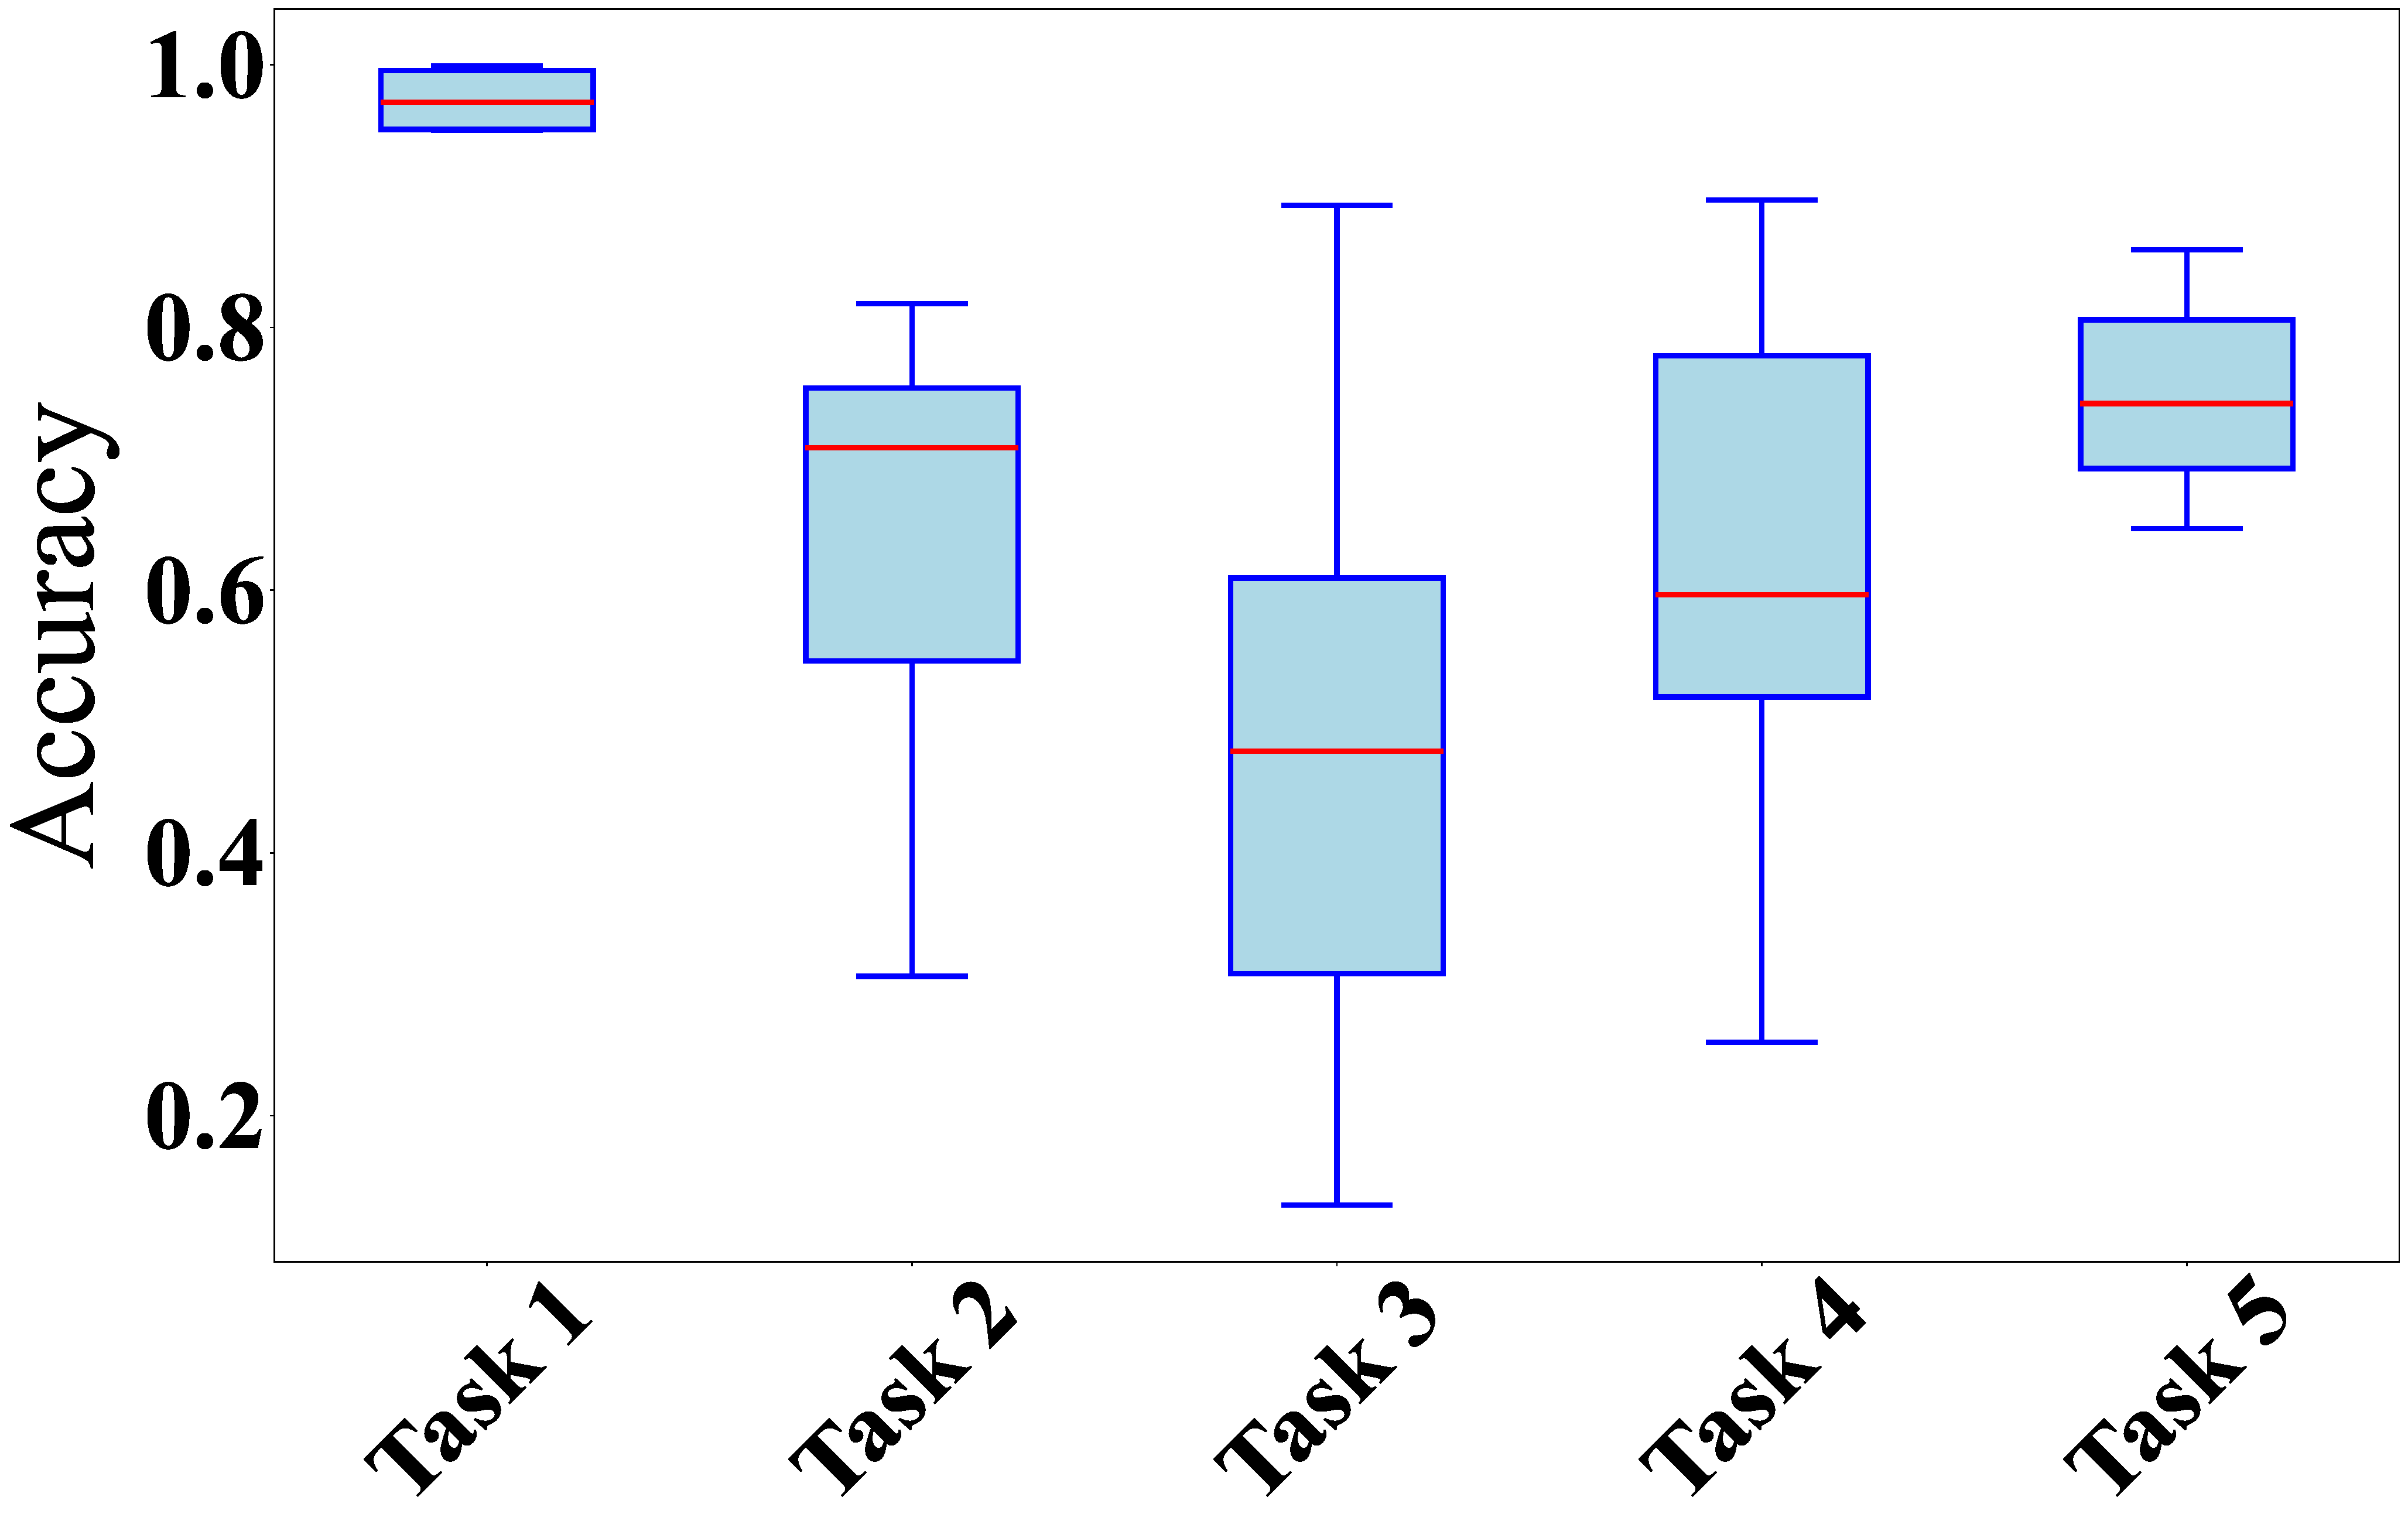
\includegraphics[width=\linewidth]{figures/box_plots/ewc_image.pdf} &
        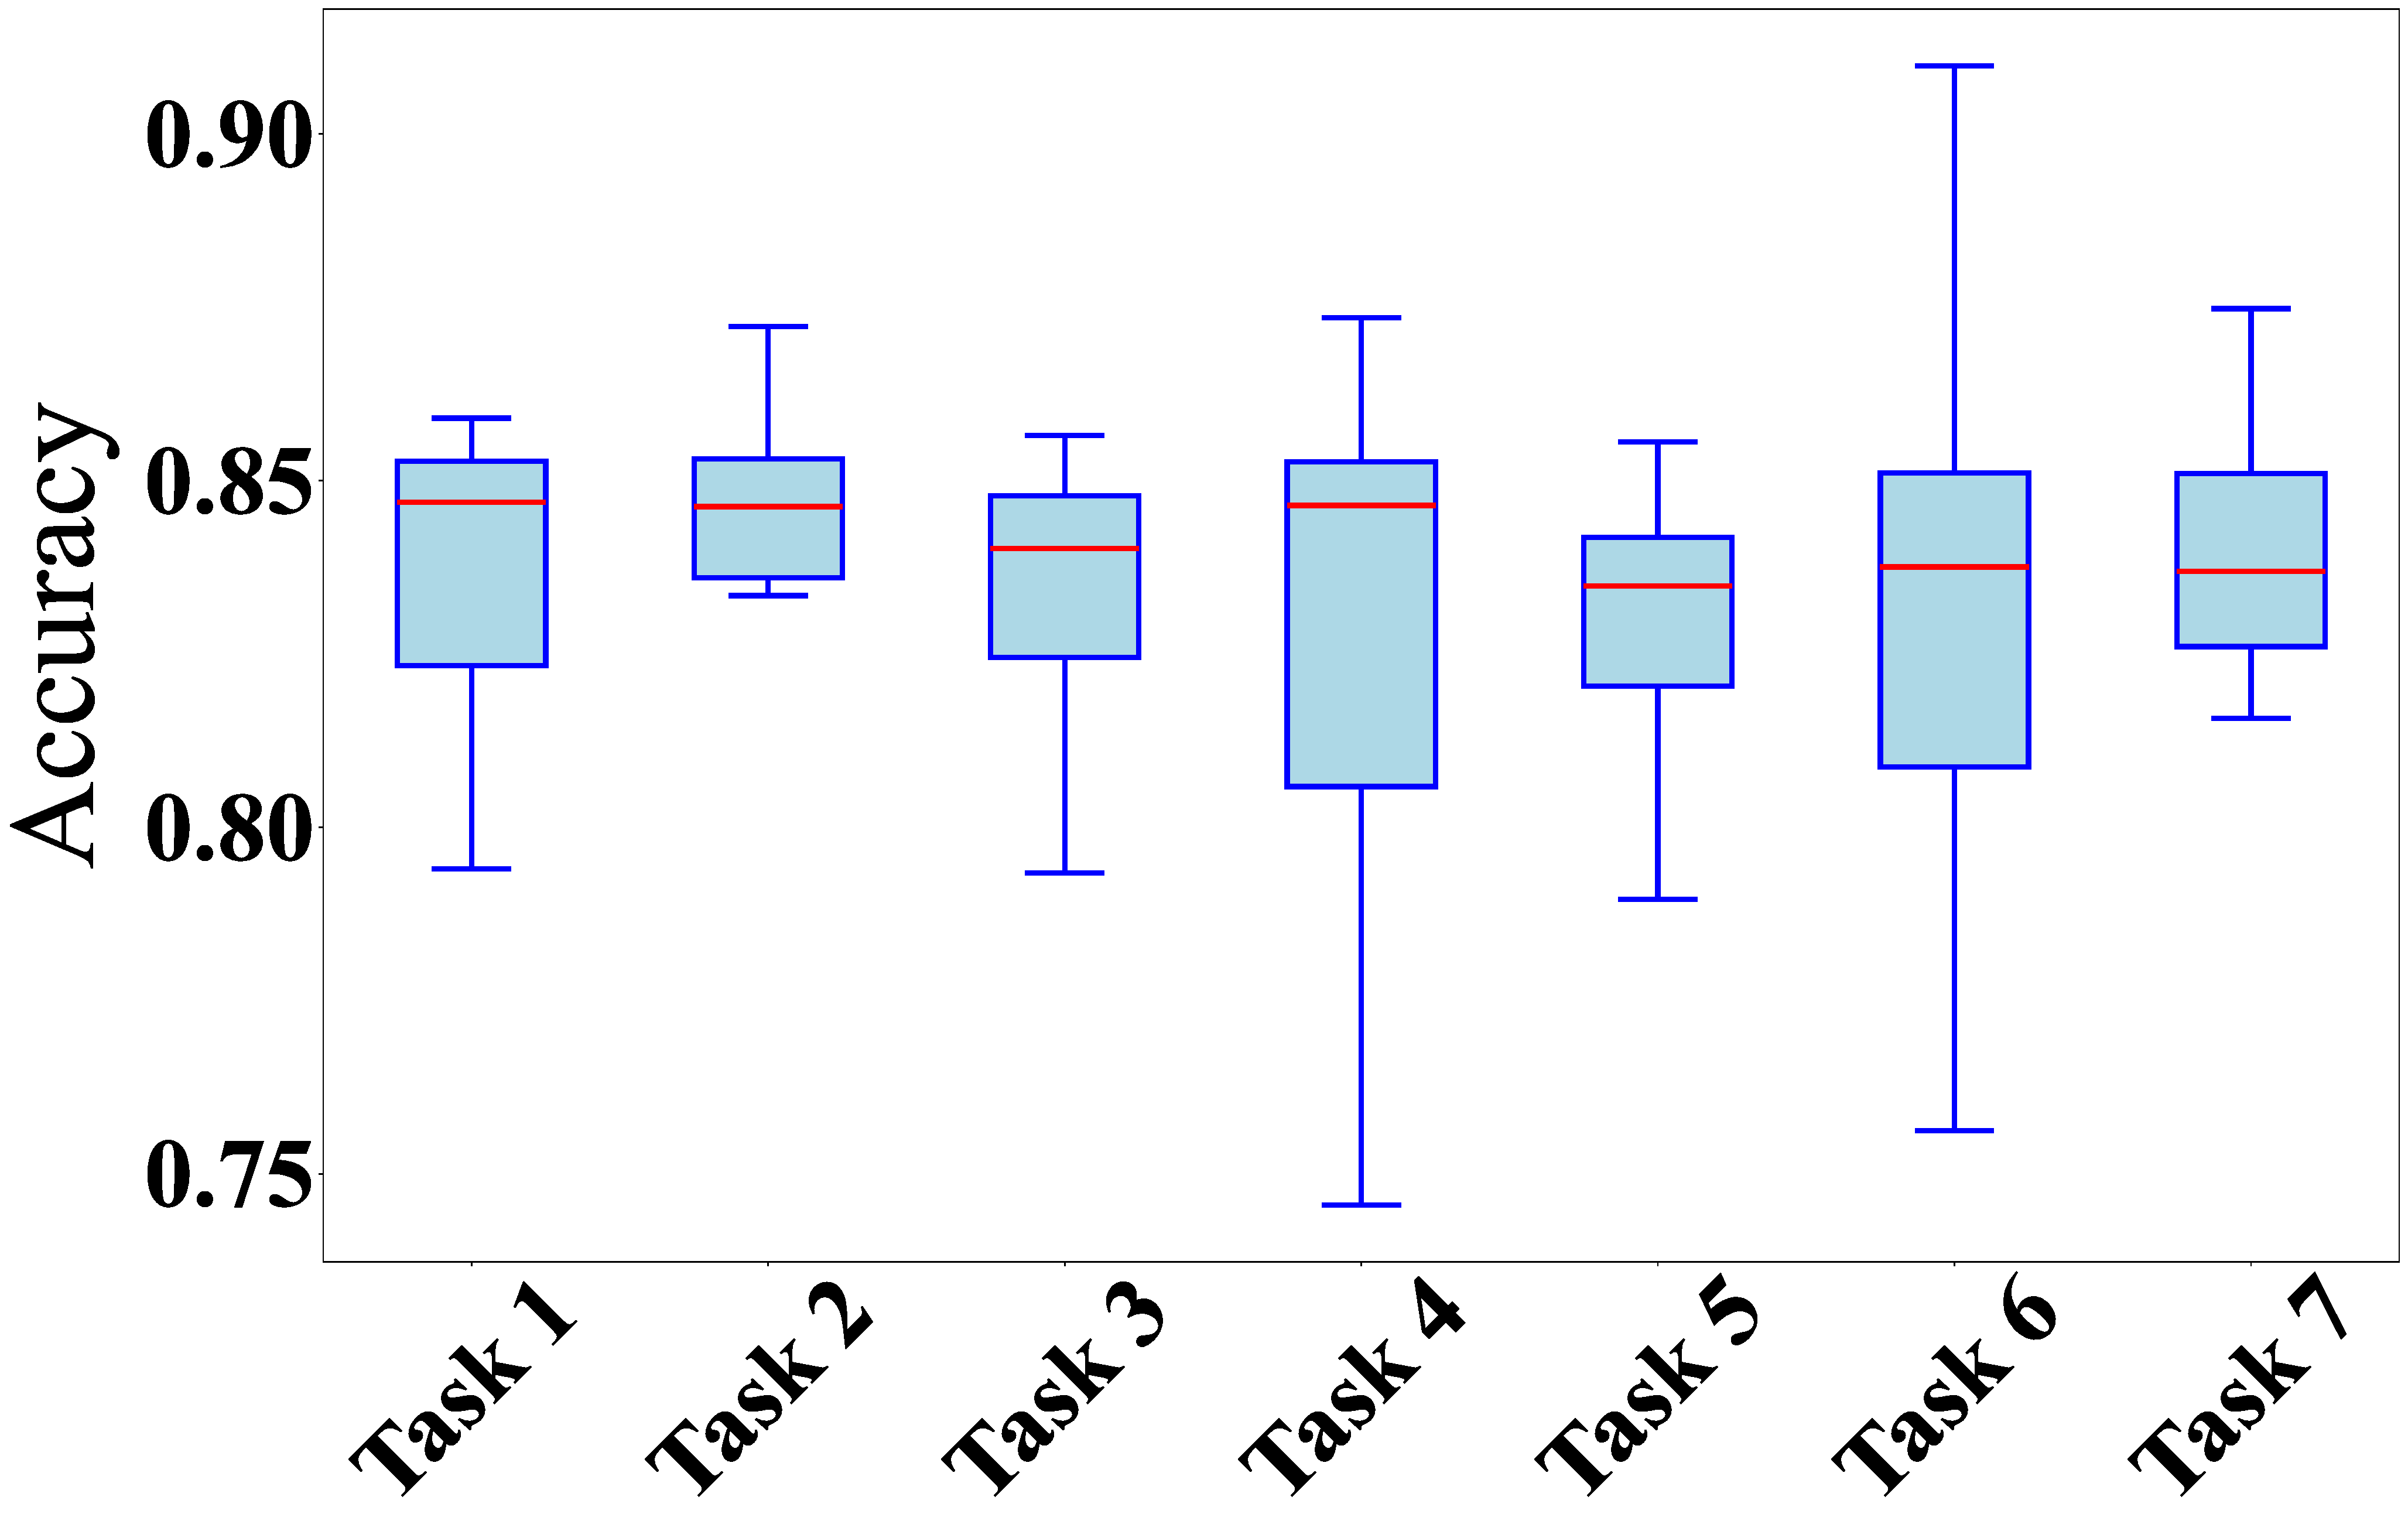
\includegraphics[width=\linewidth]{figures/box_plots/ewc_text.pdf} &
        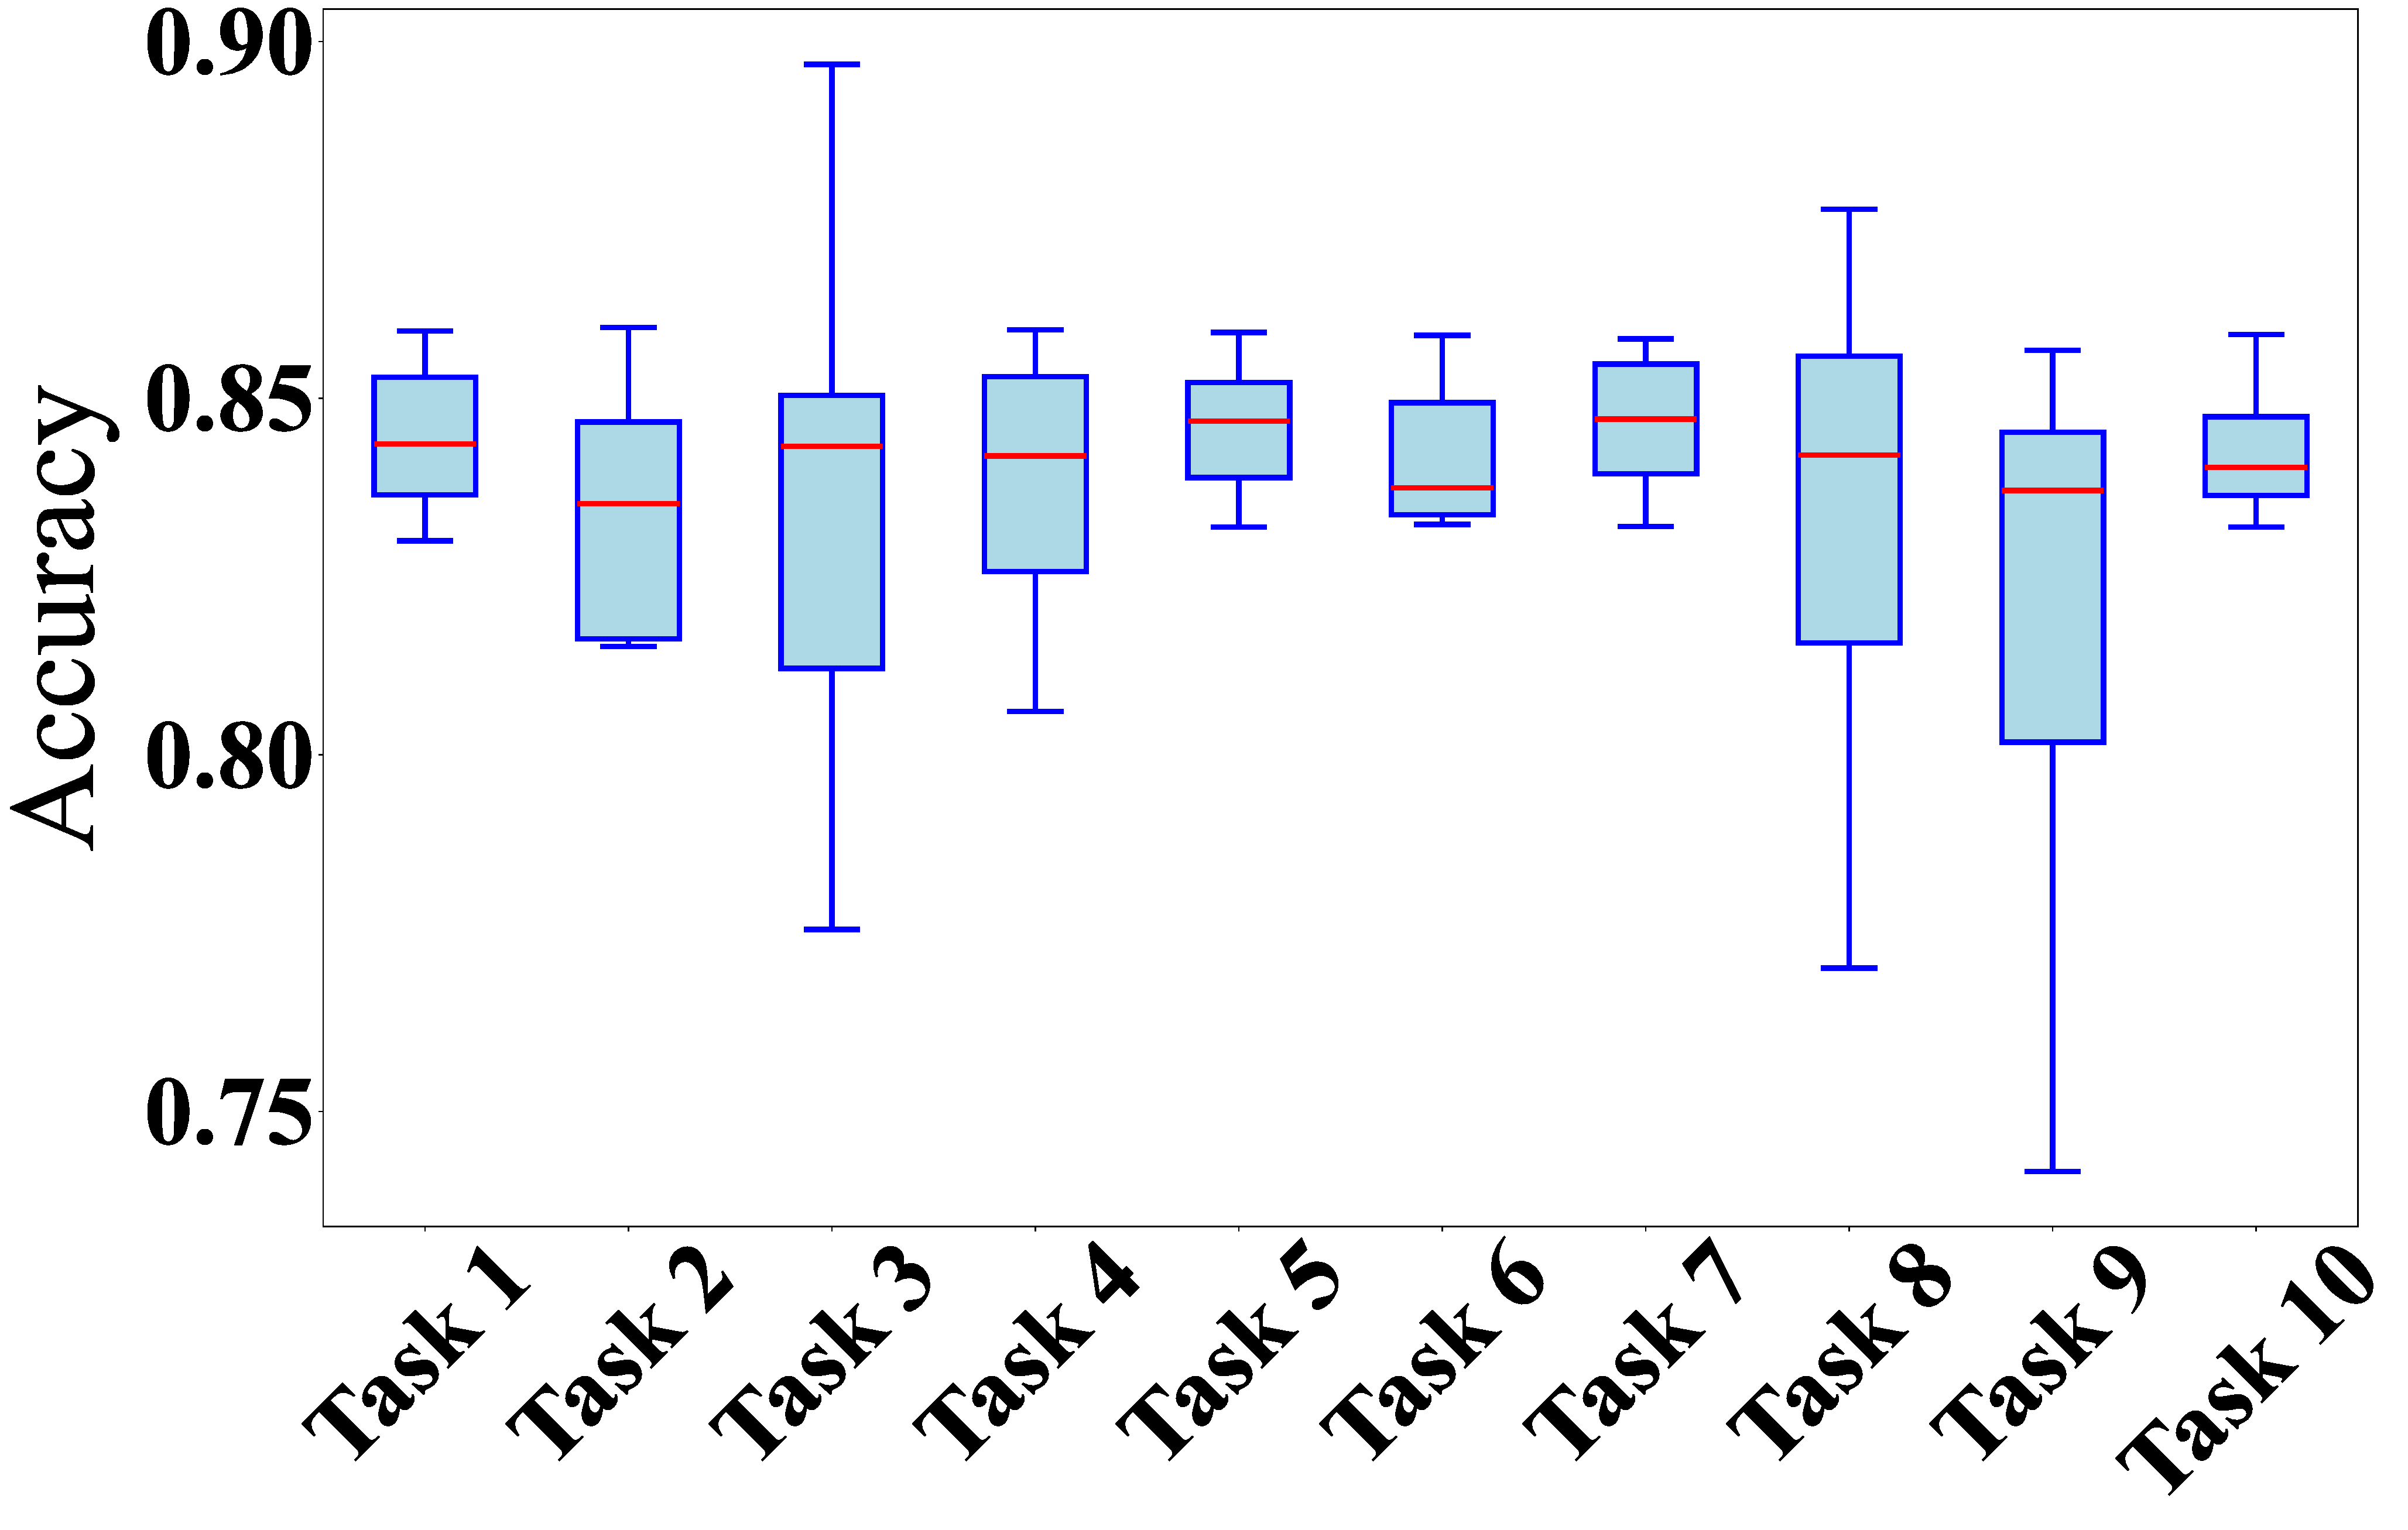
\includegraphics[width=\linewidth]{figures/box_plots/ewc_graph.pdf} &
        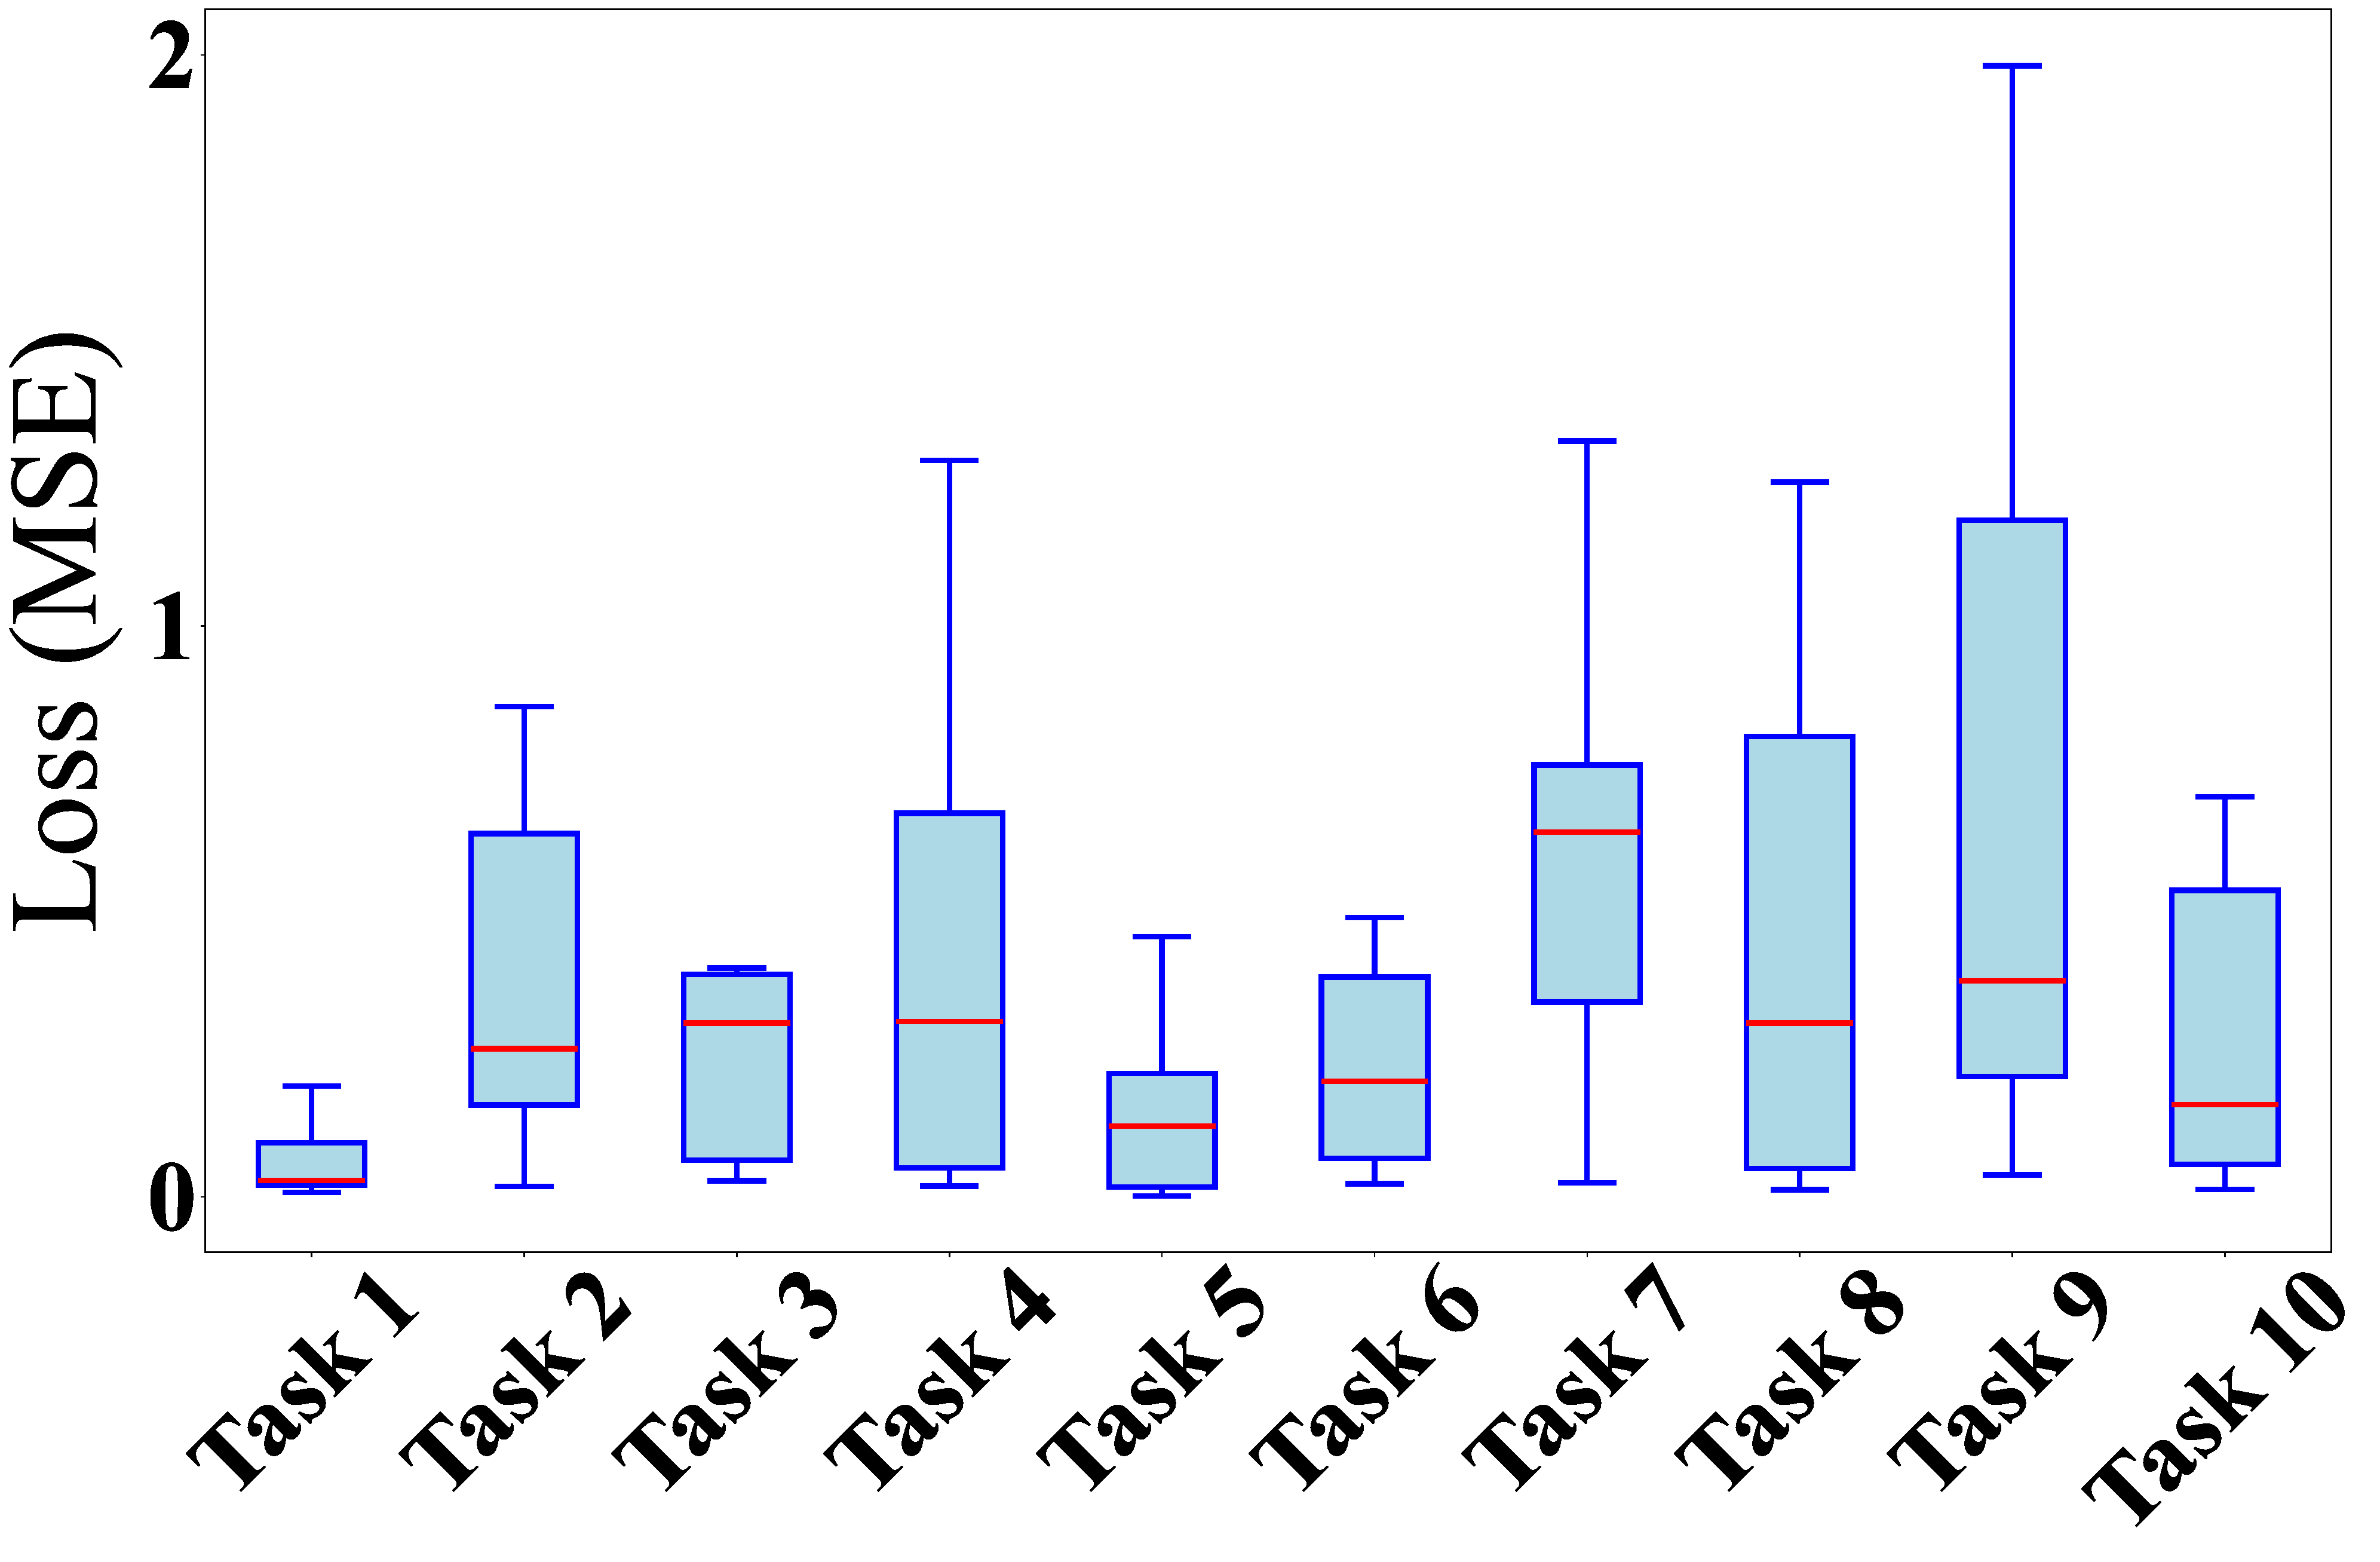
\includegraphics[width=\linewidth]{figures/box_plots/ewc_sine.pdf} \\
        \textbf{ER} &
        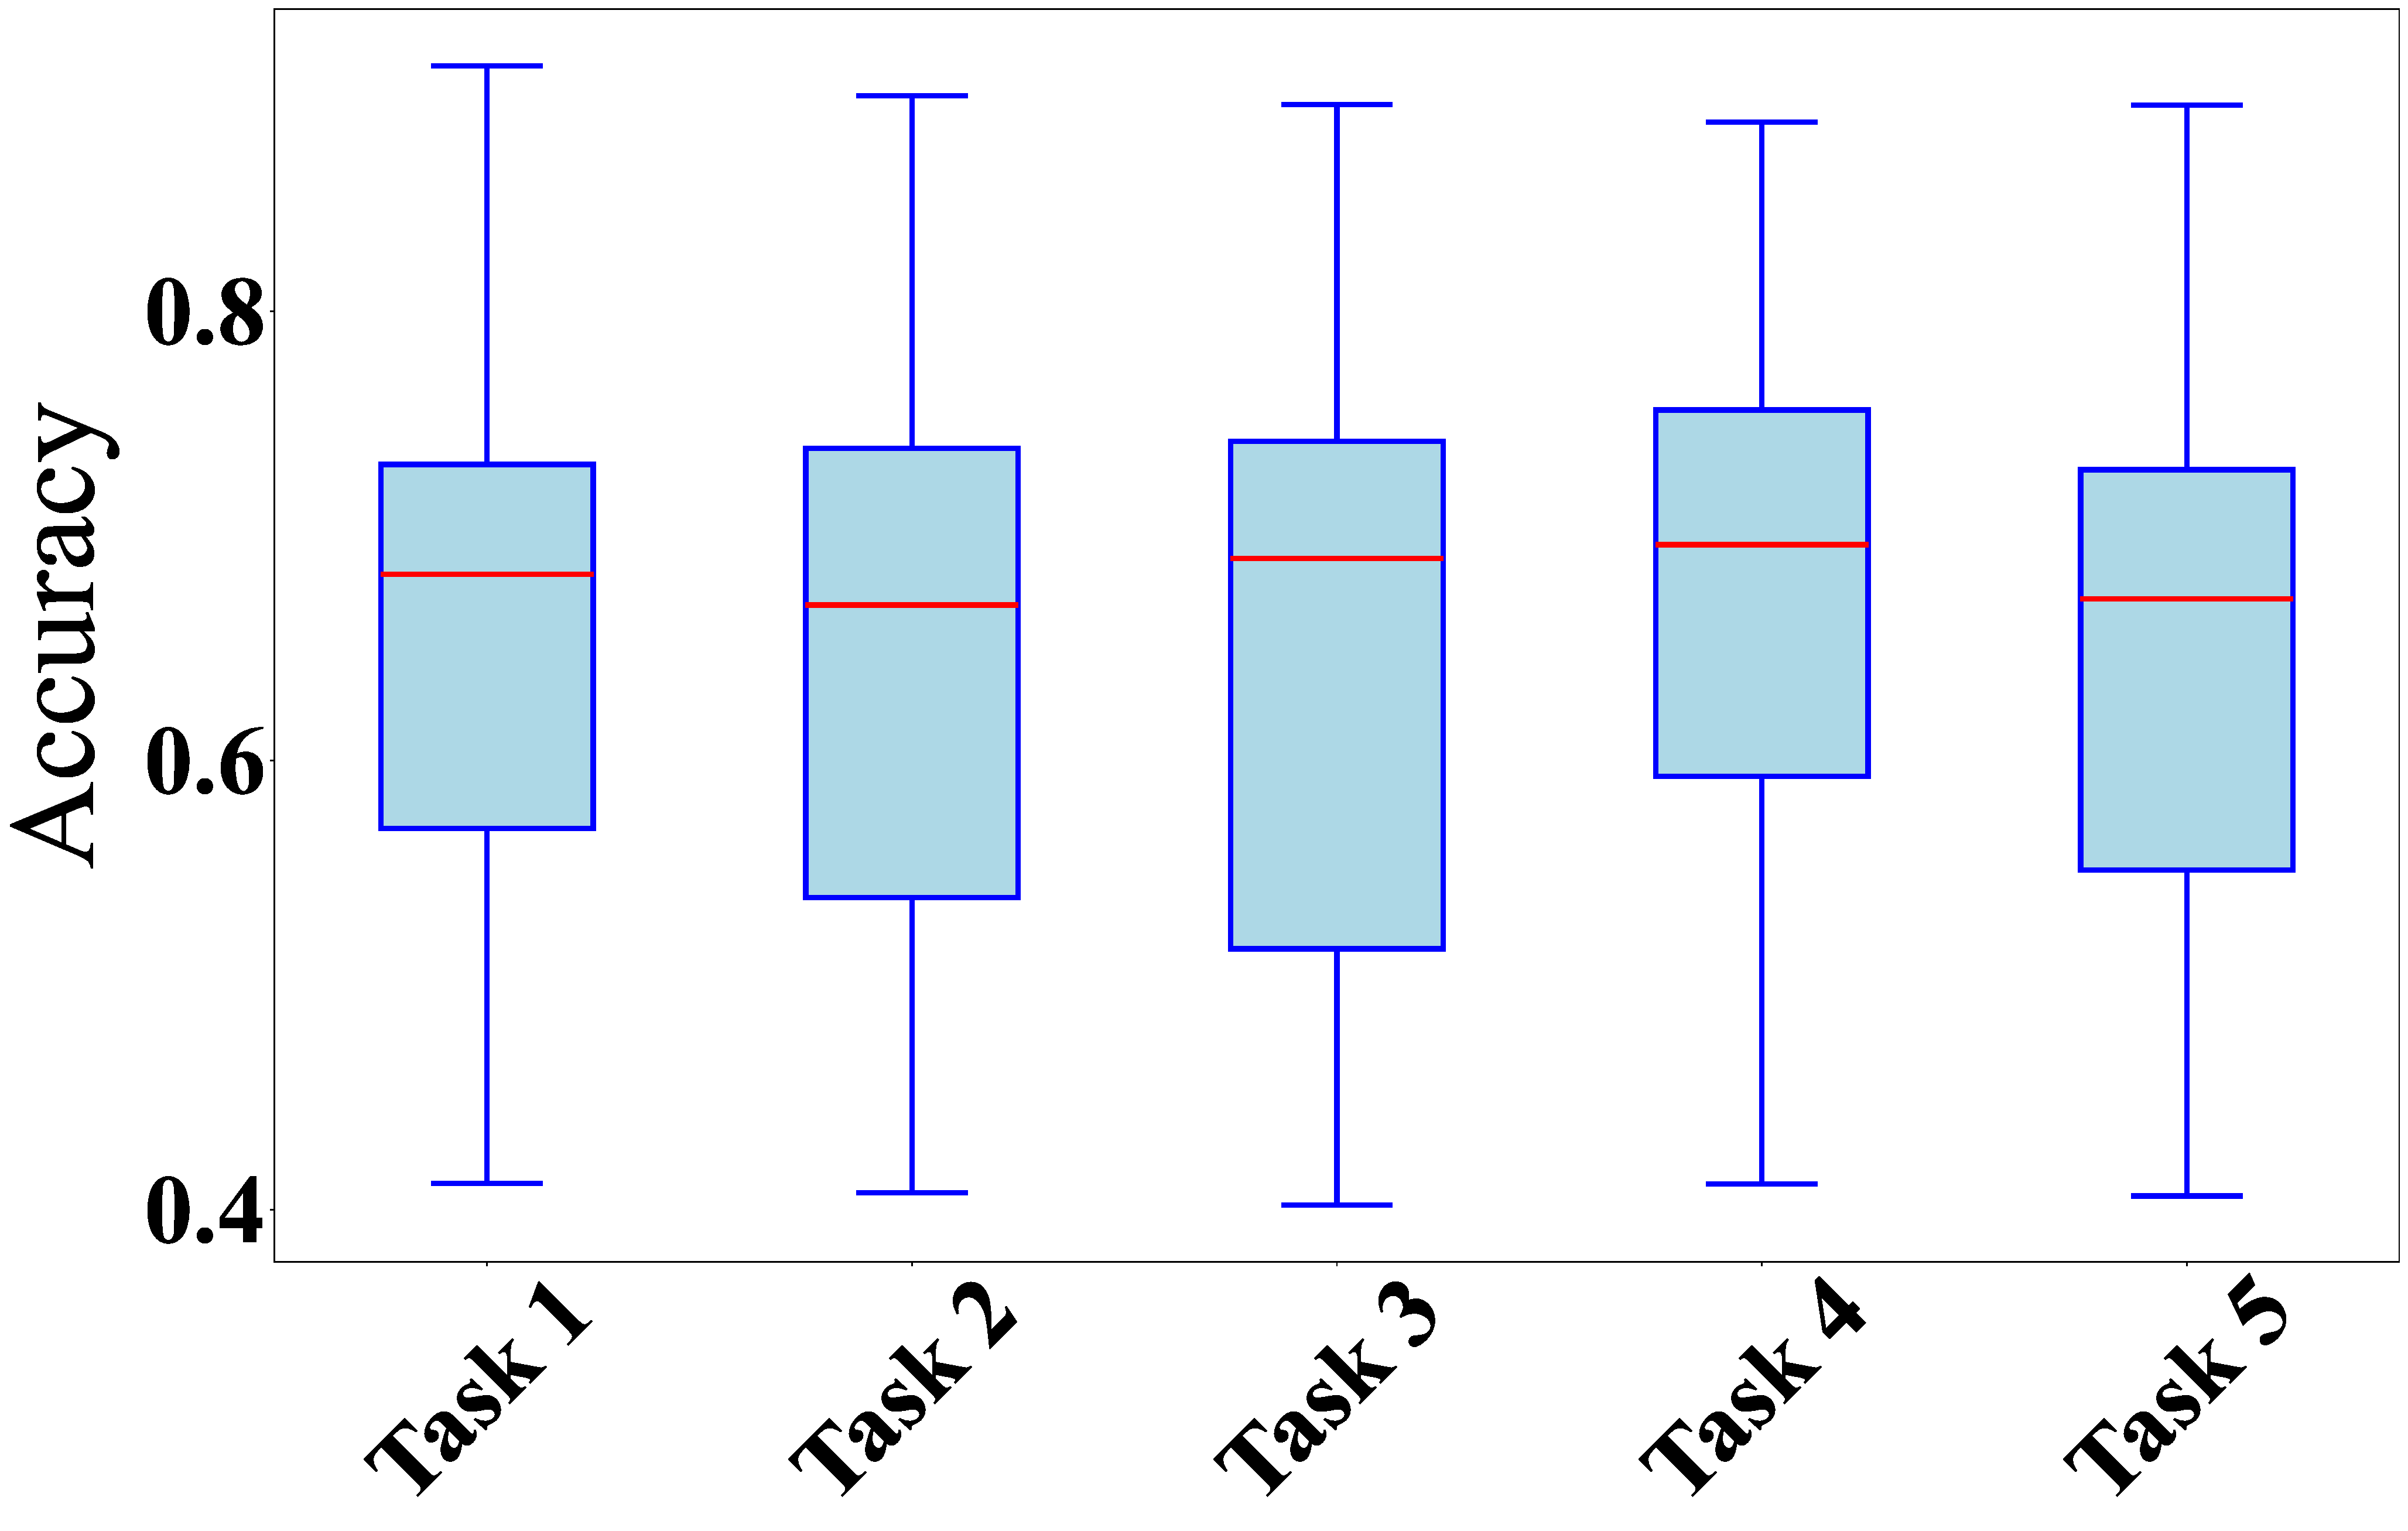
\includegraphics[width=\linewidth]{figures/box_plots/mr_image.pdf} &
        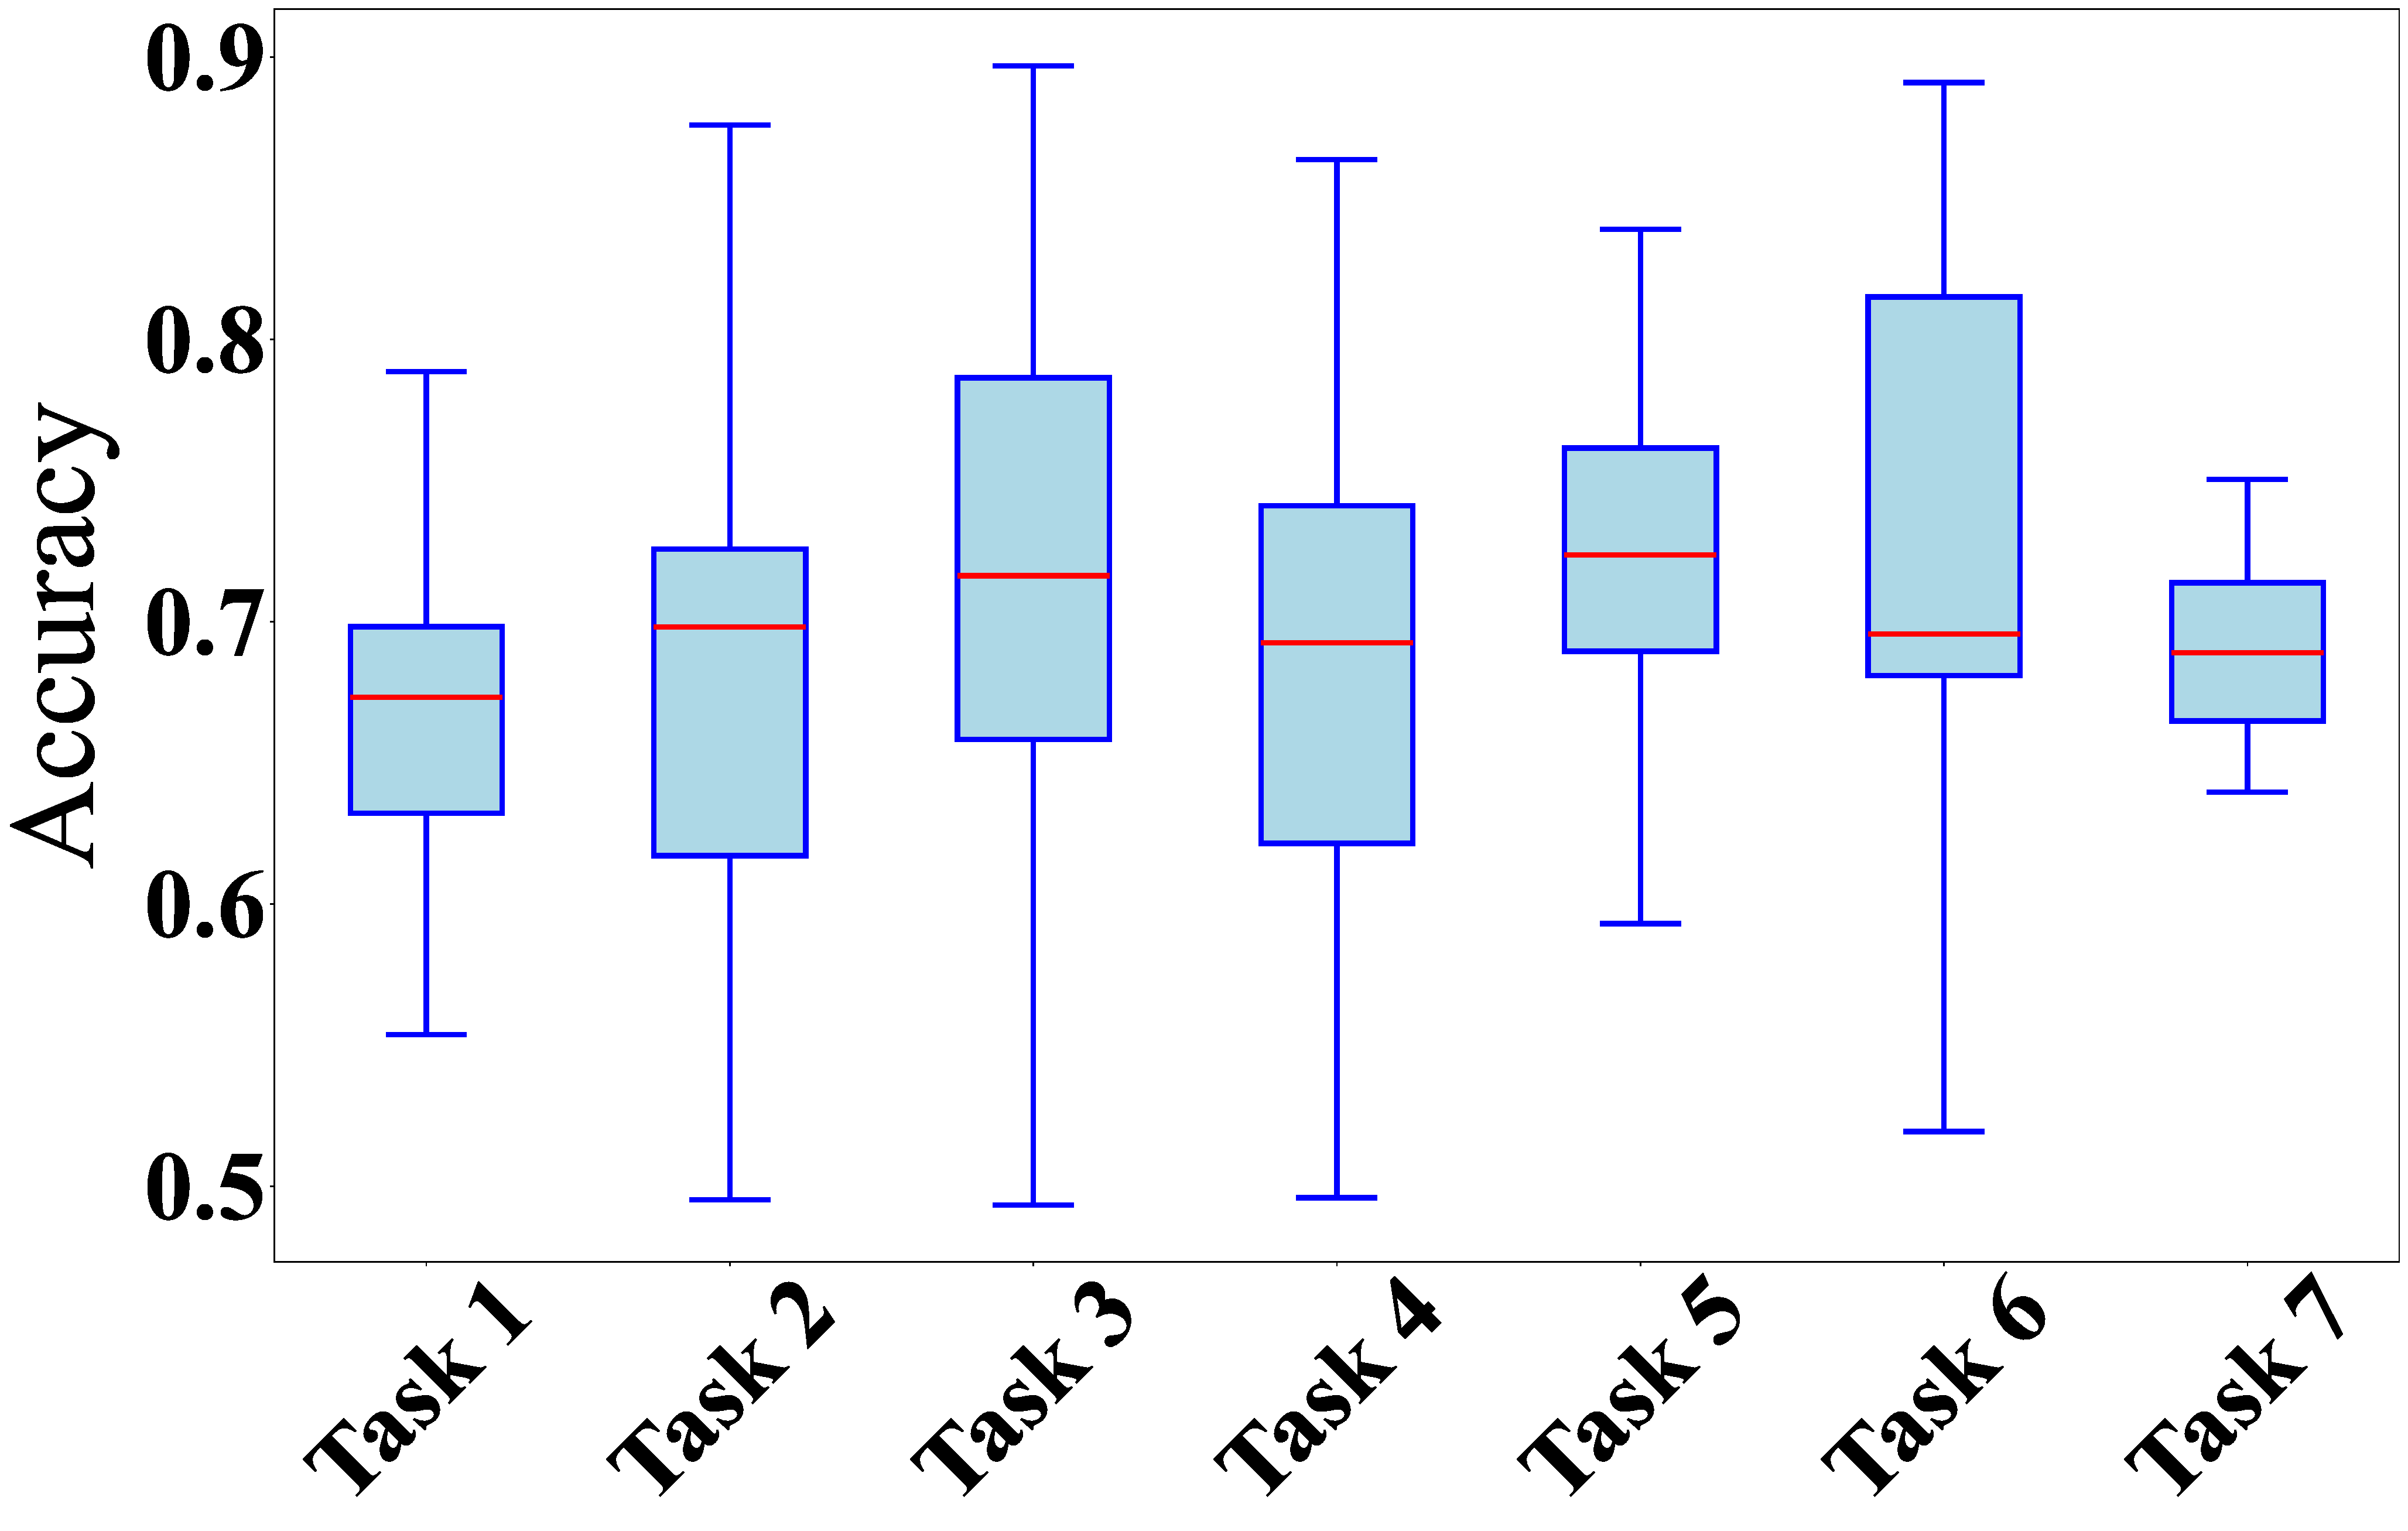
\includegraphics[width=\linewidth]{figures/box_plots/mr_text.pdf} &
        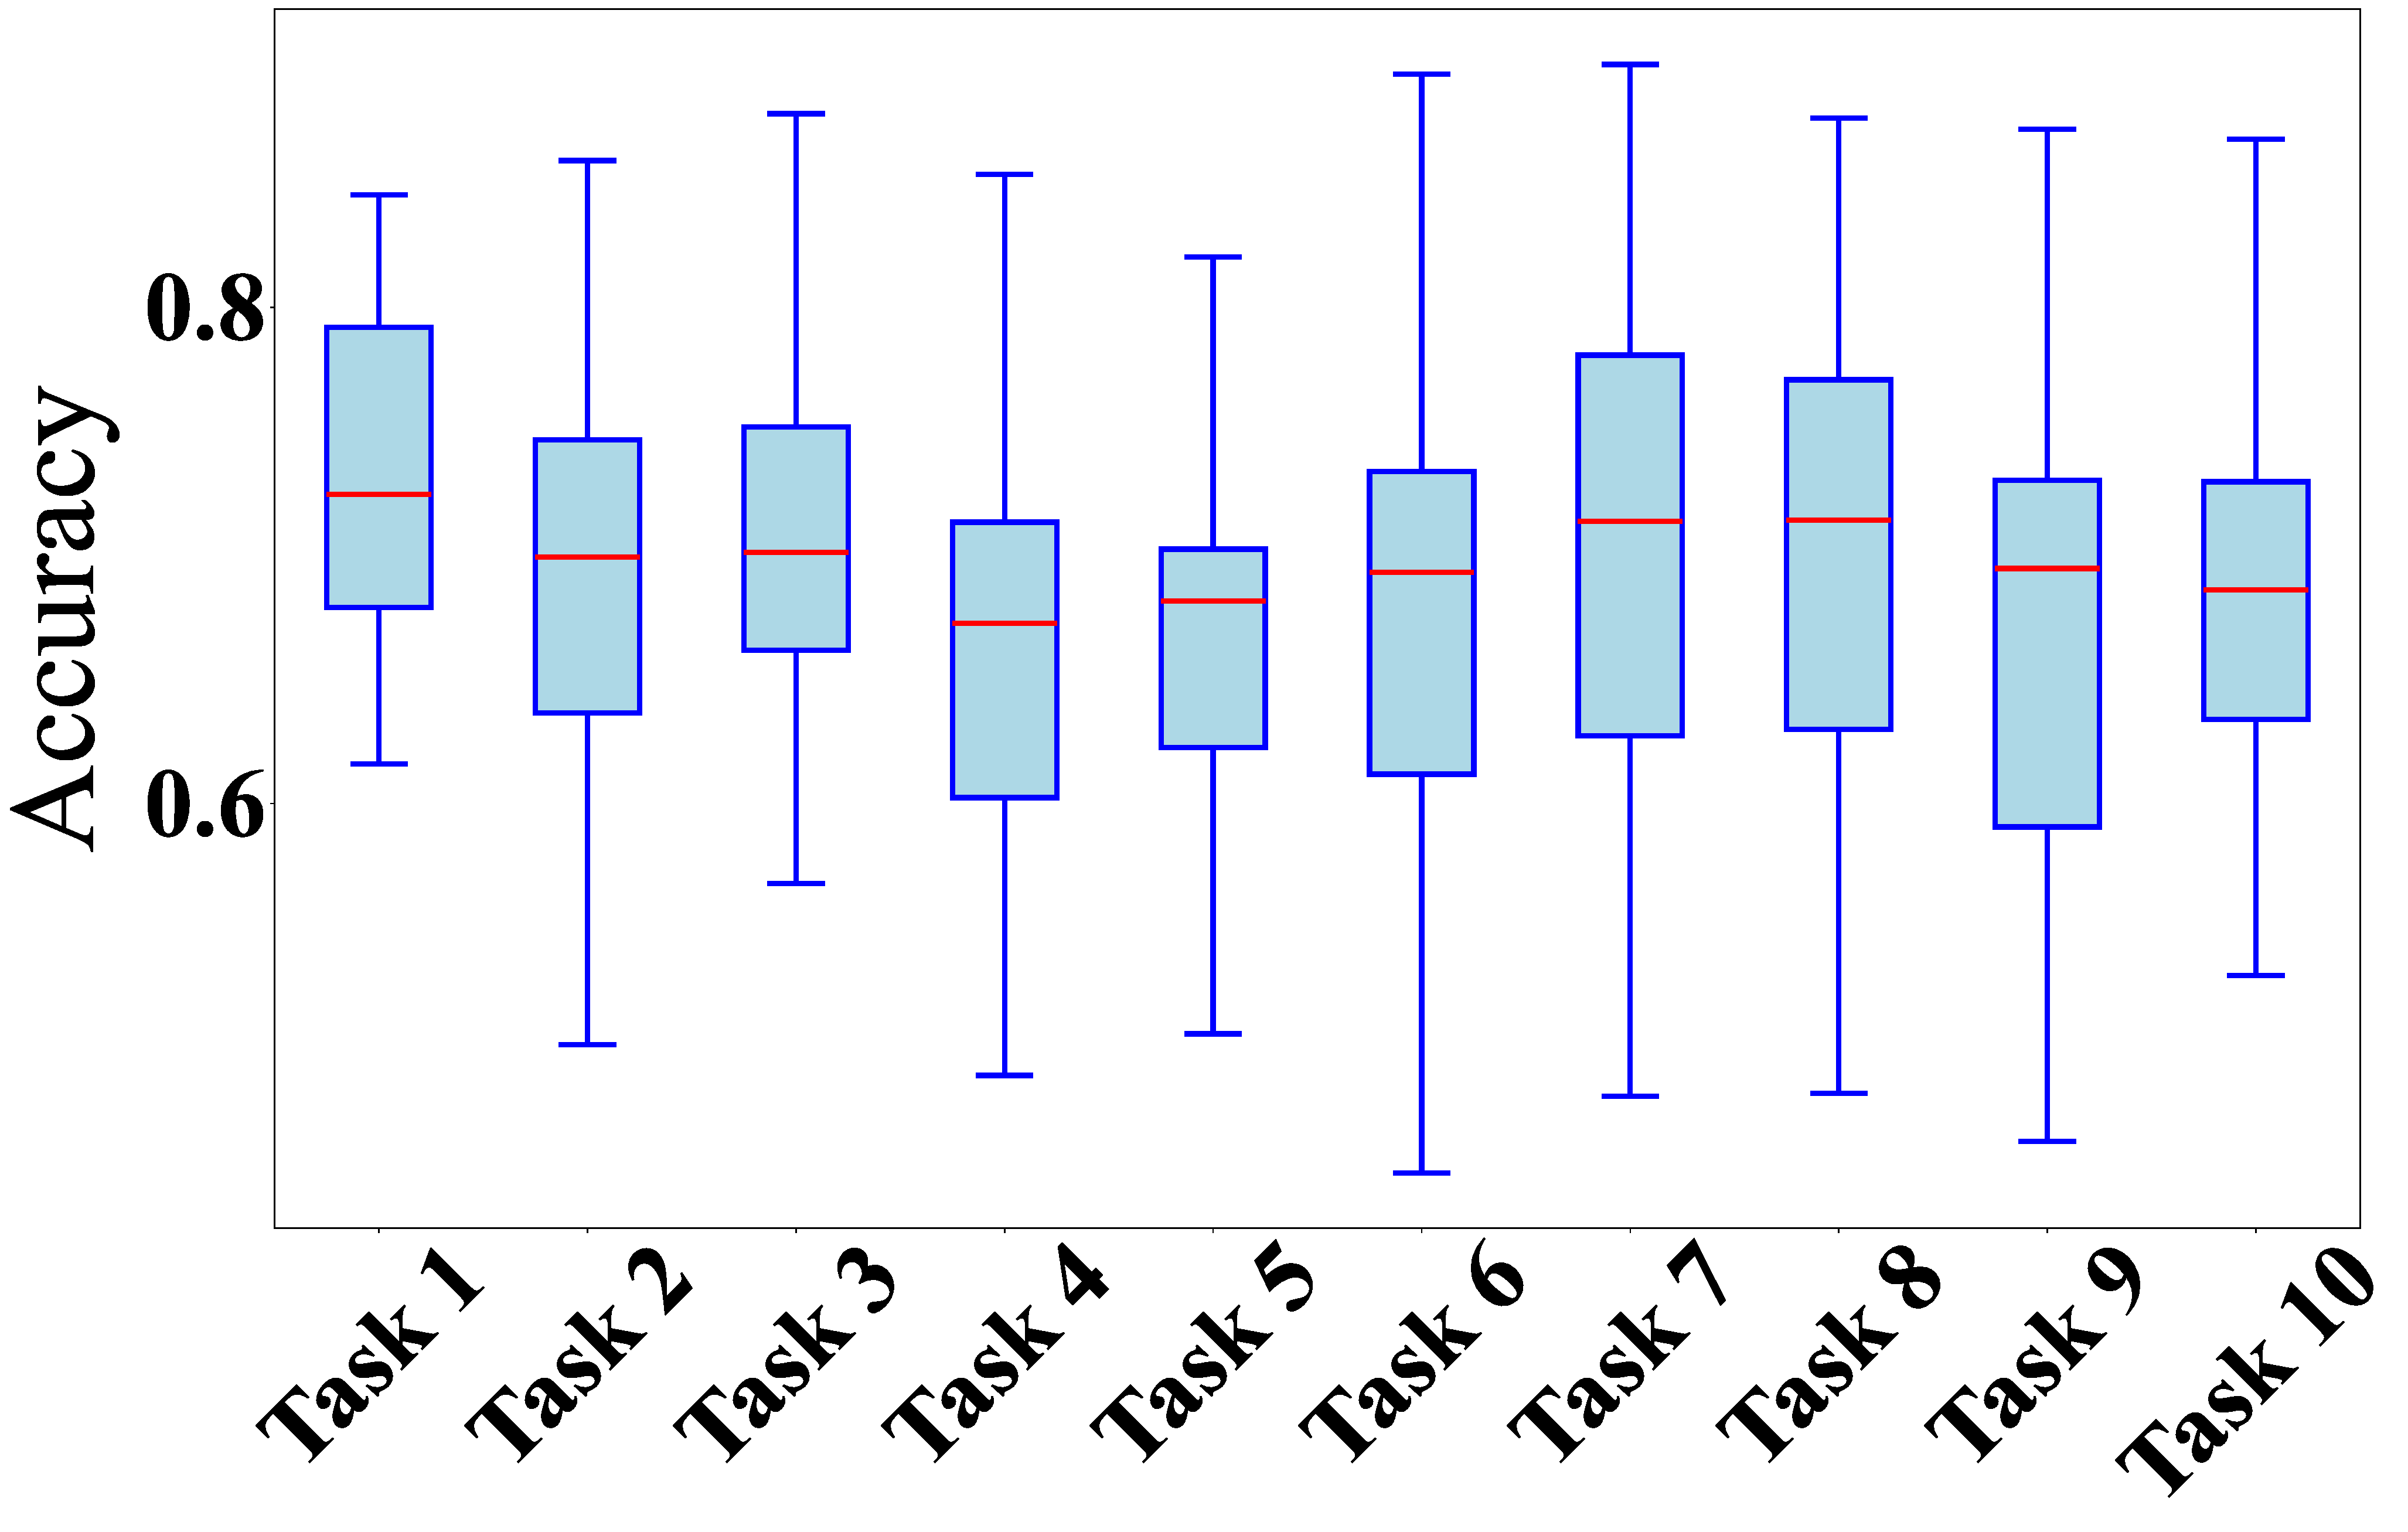
\includegraphics[width=\linewidth]{figures/box_plots/mr_graph.pdf} &
        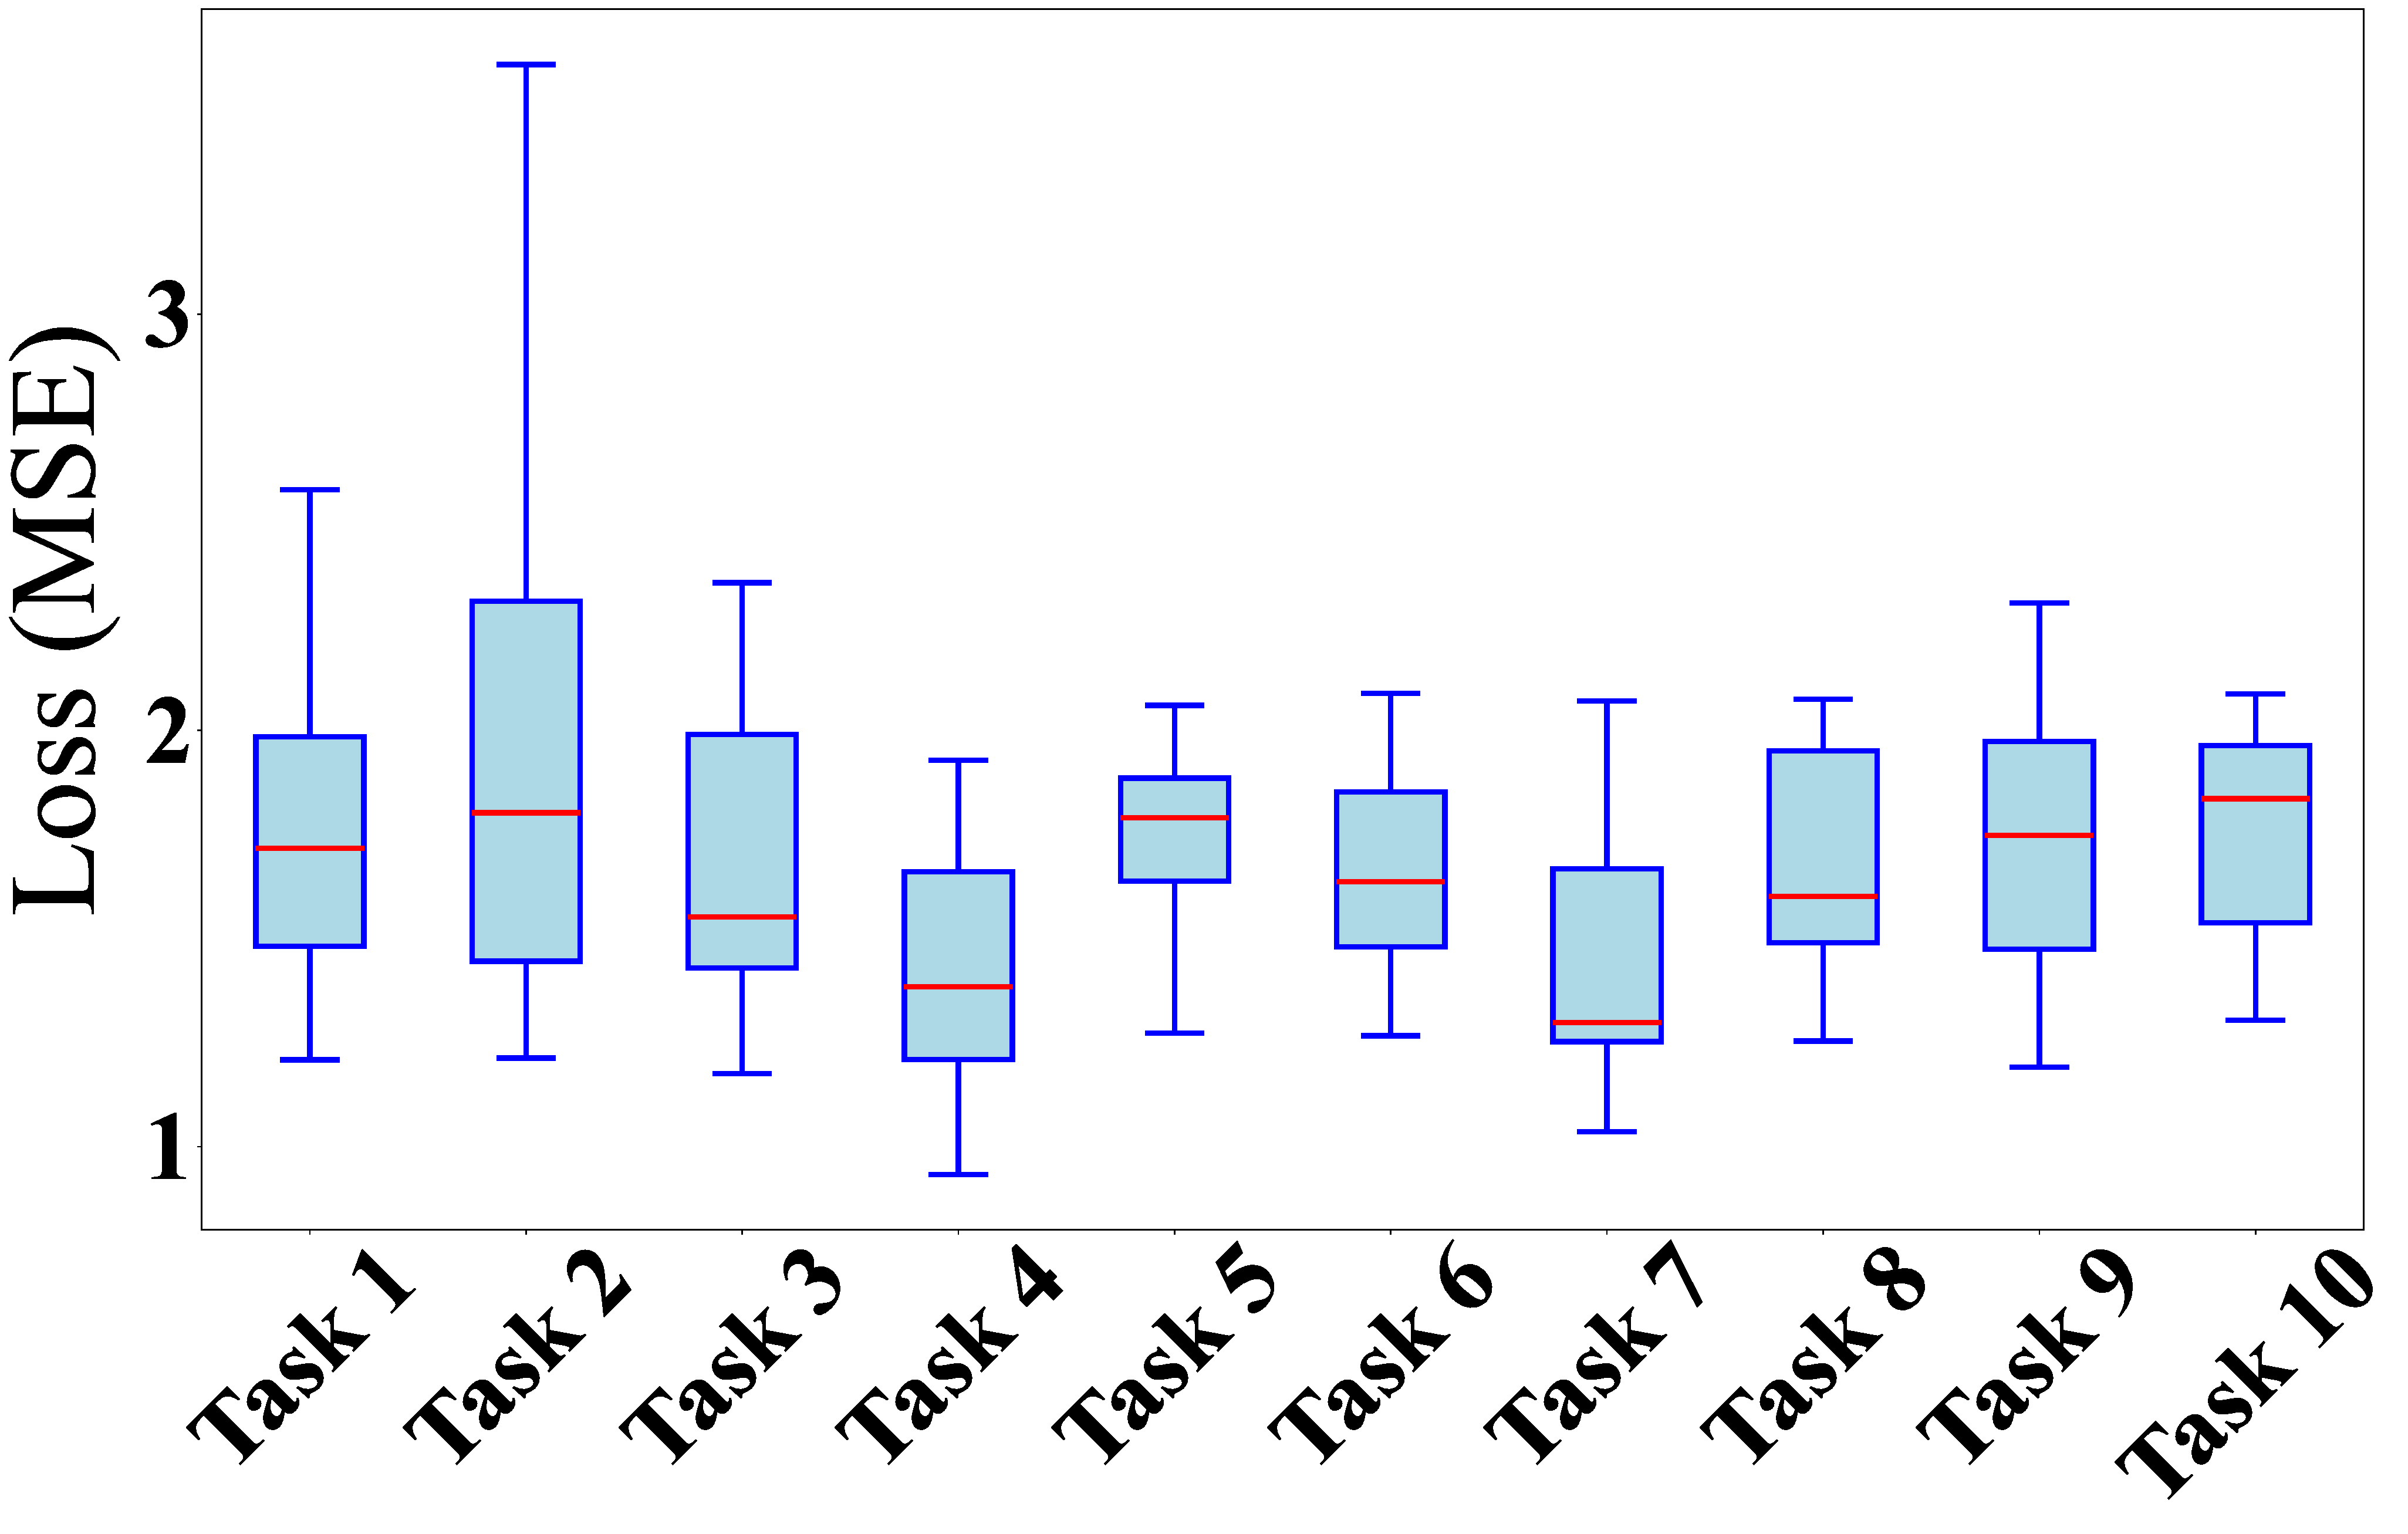
\includegraphics[width=\linewidth]{figures/box_plots/mr_sine.pdf} \\
        \textbf{BCL} &
        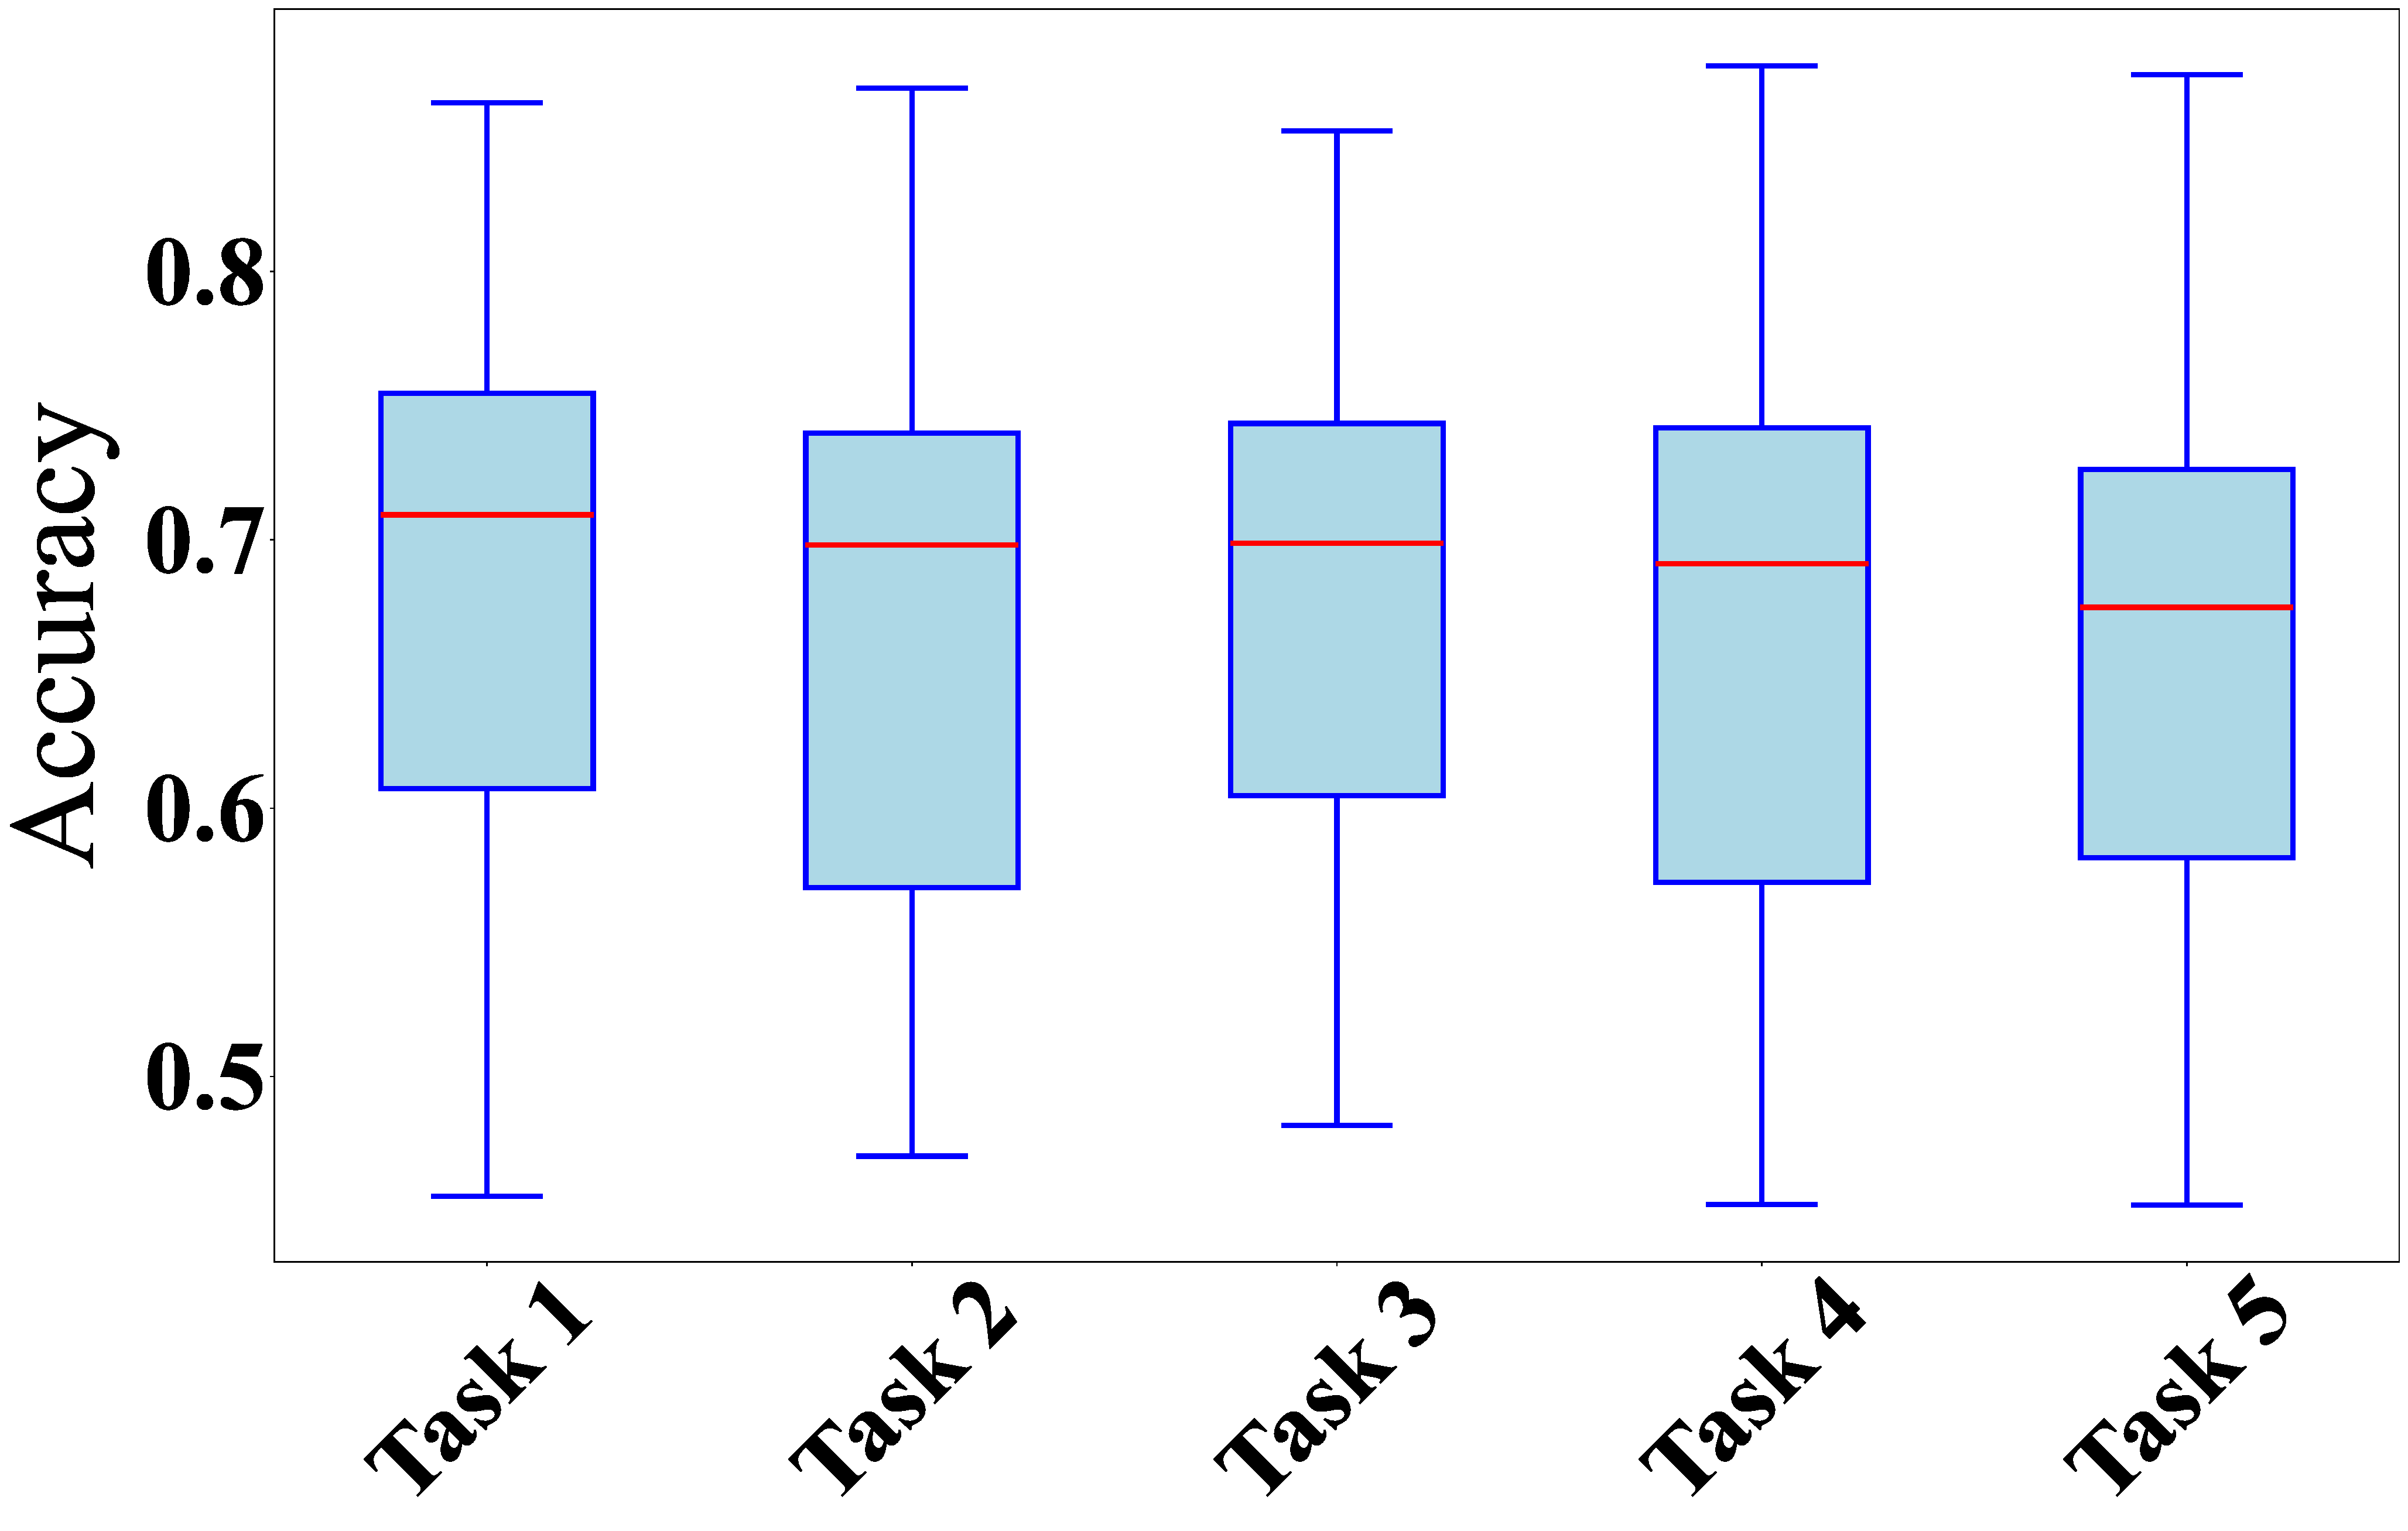
\includegraphics[width=\linewidth]{figures/box_plots/bcl_image.pdf} &
        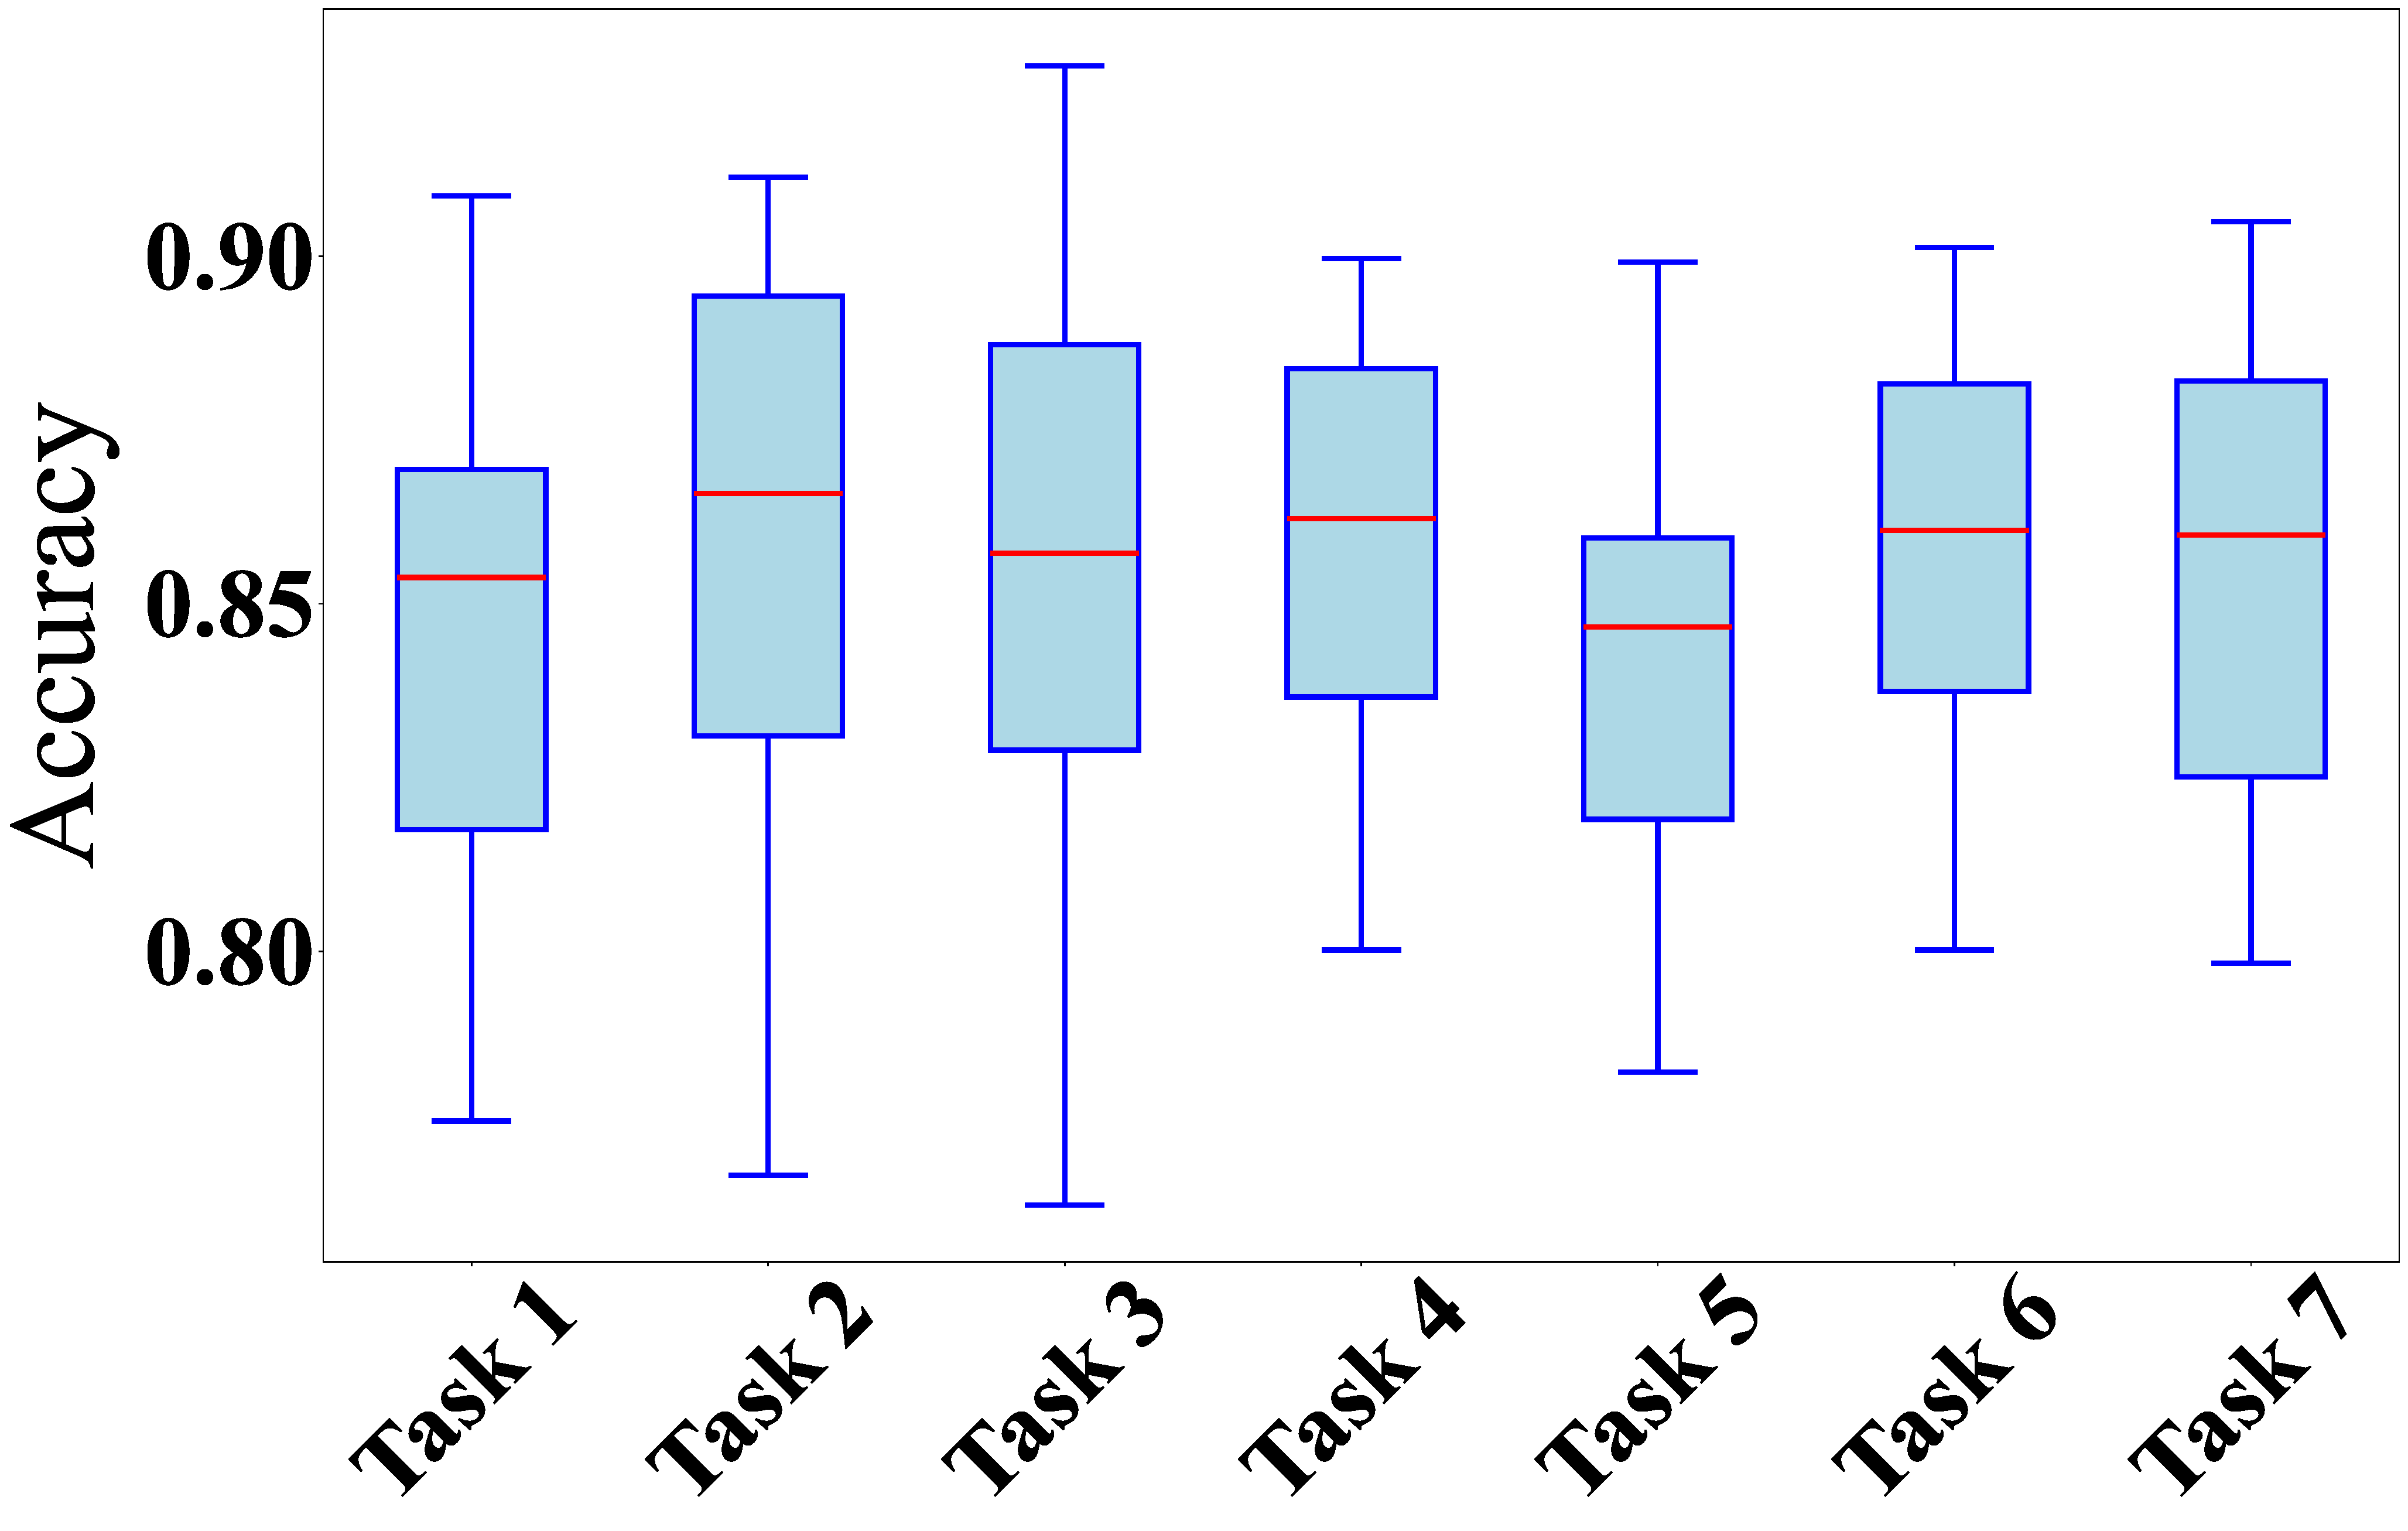
\includegraphics[width=\linewidth]{figures/box_plots/bcl_text.pdf} &
        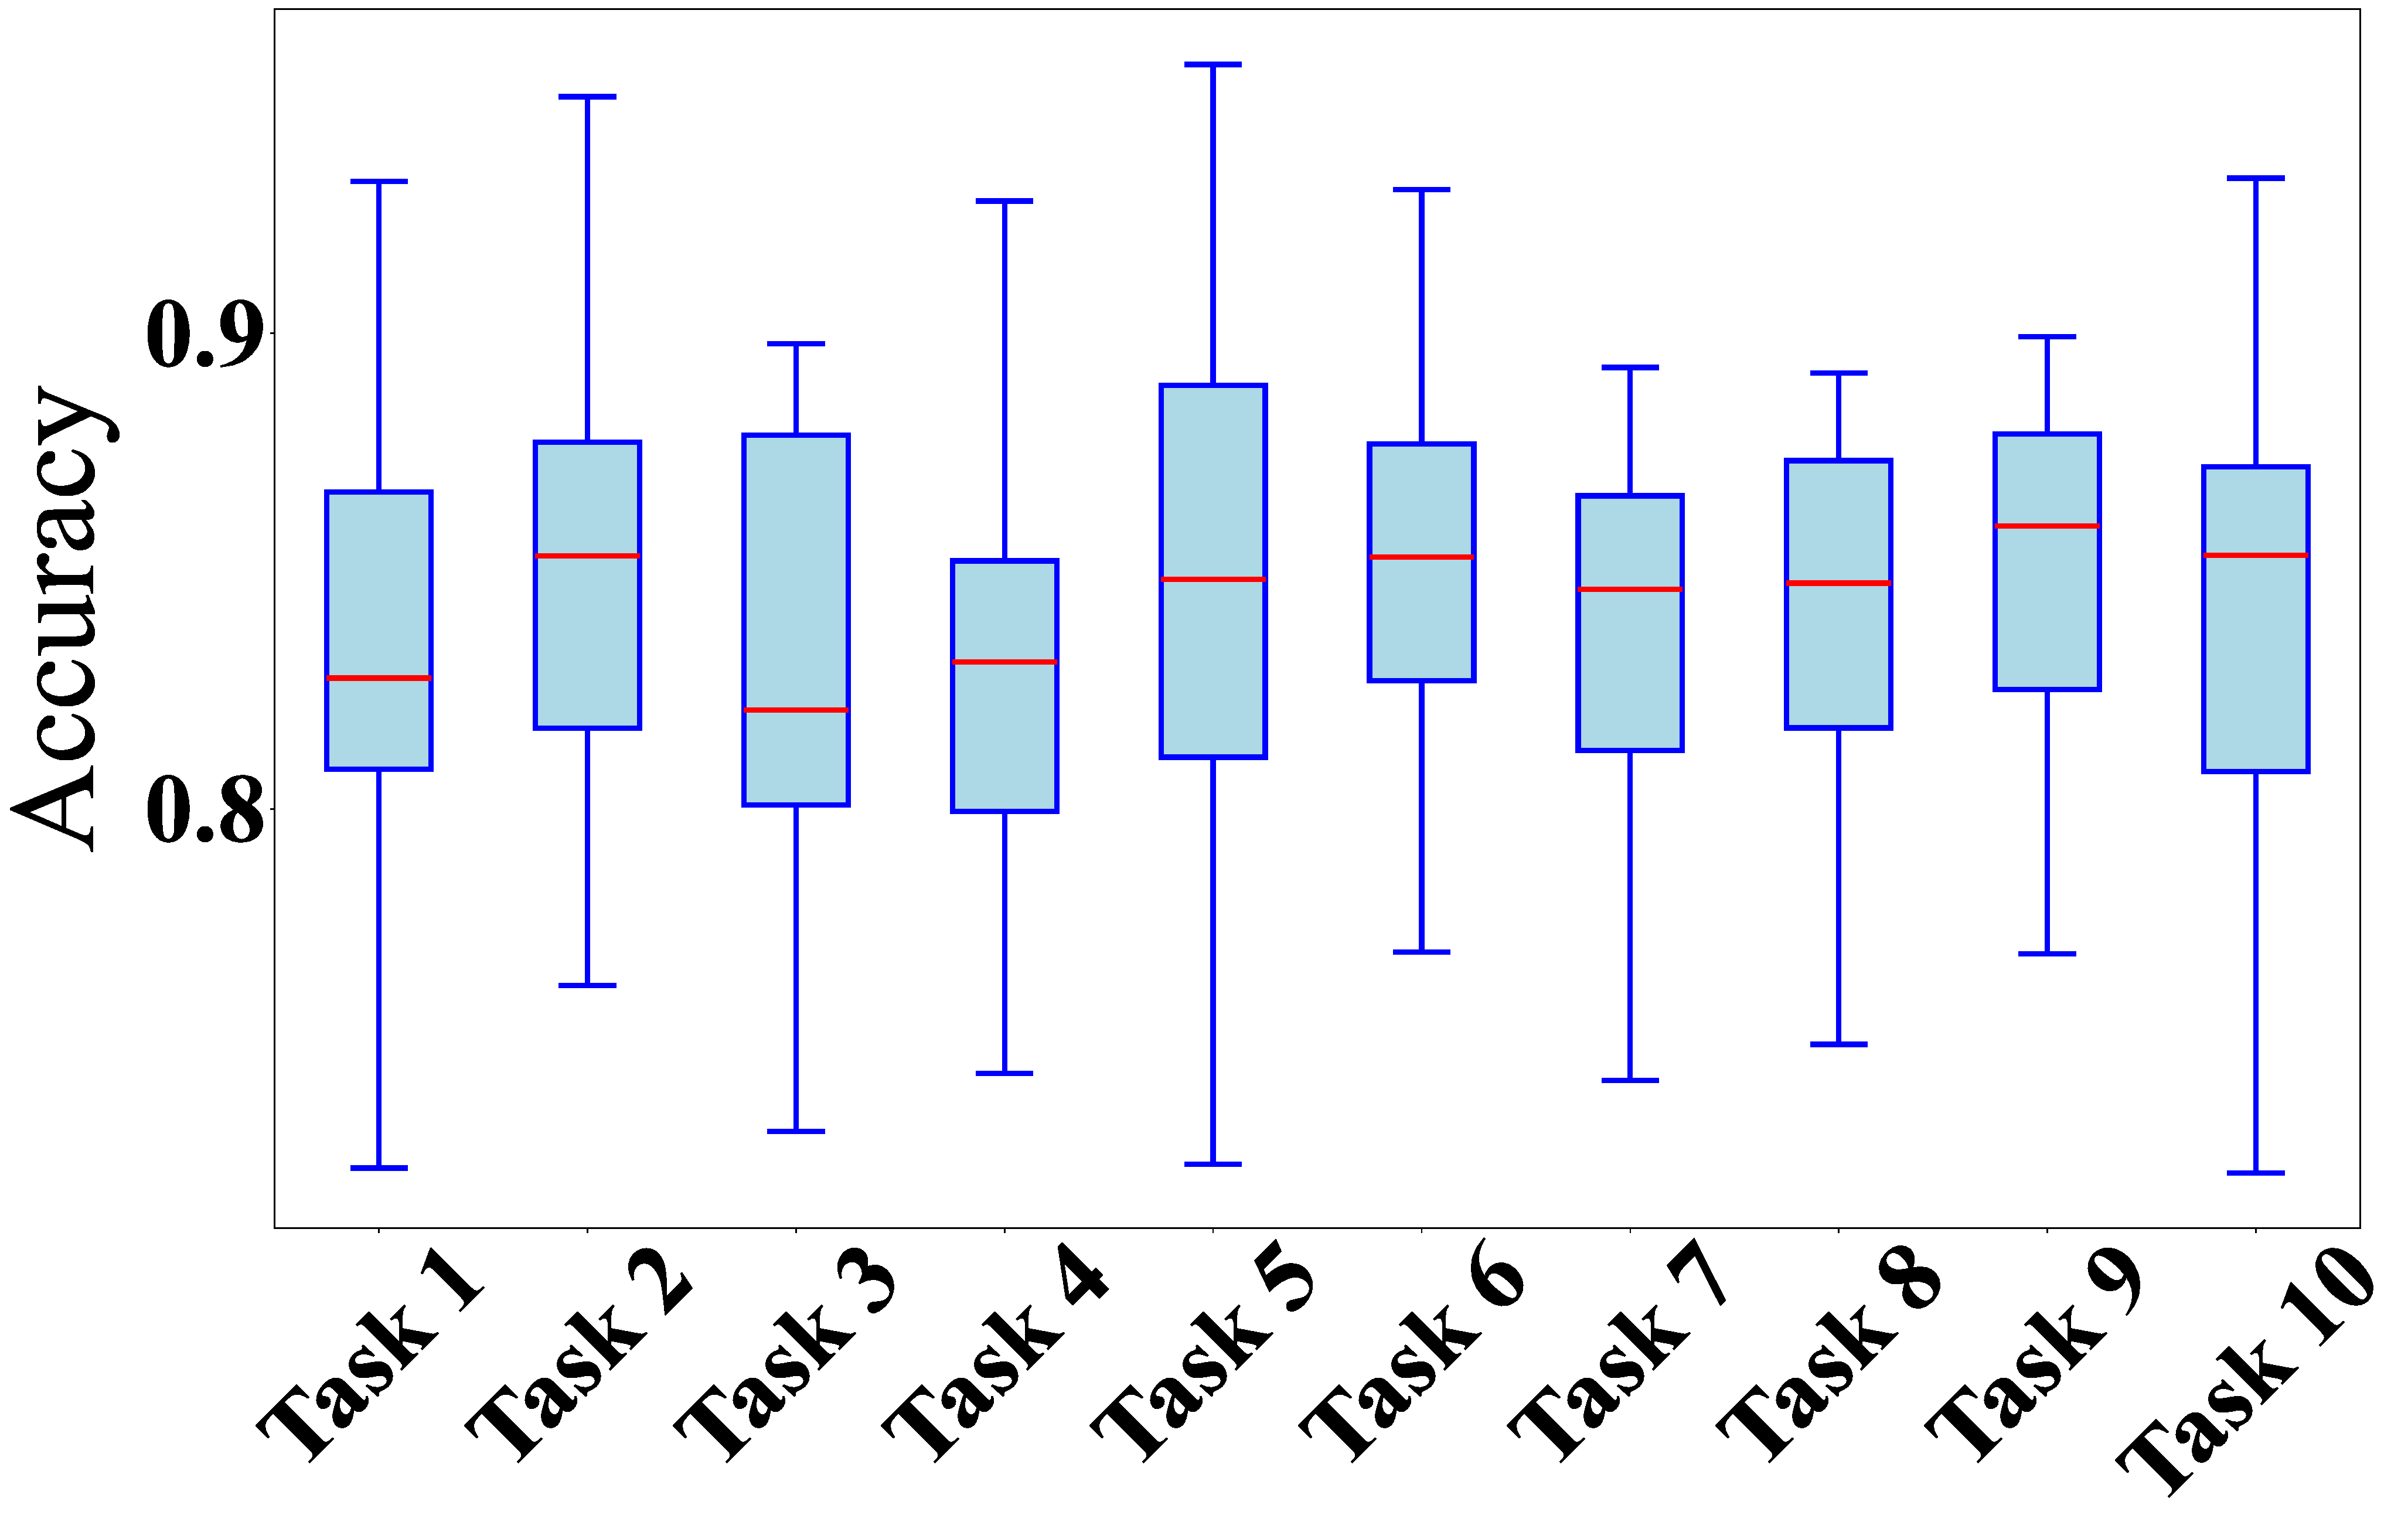
\includegraphics[width=\linewidth]{figures/box_plots/bcl_graph.pdf} &
        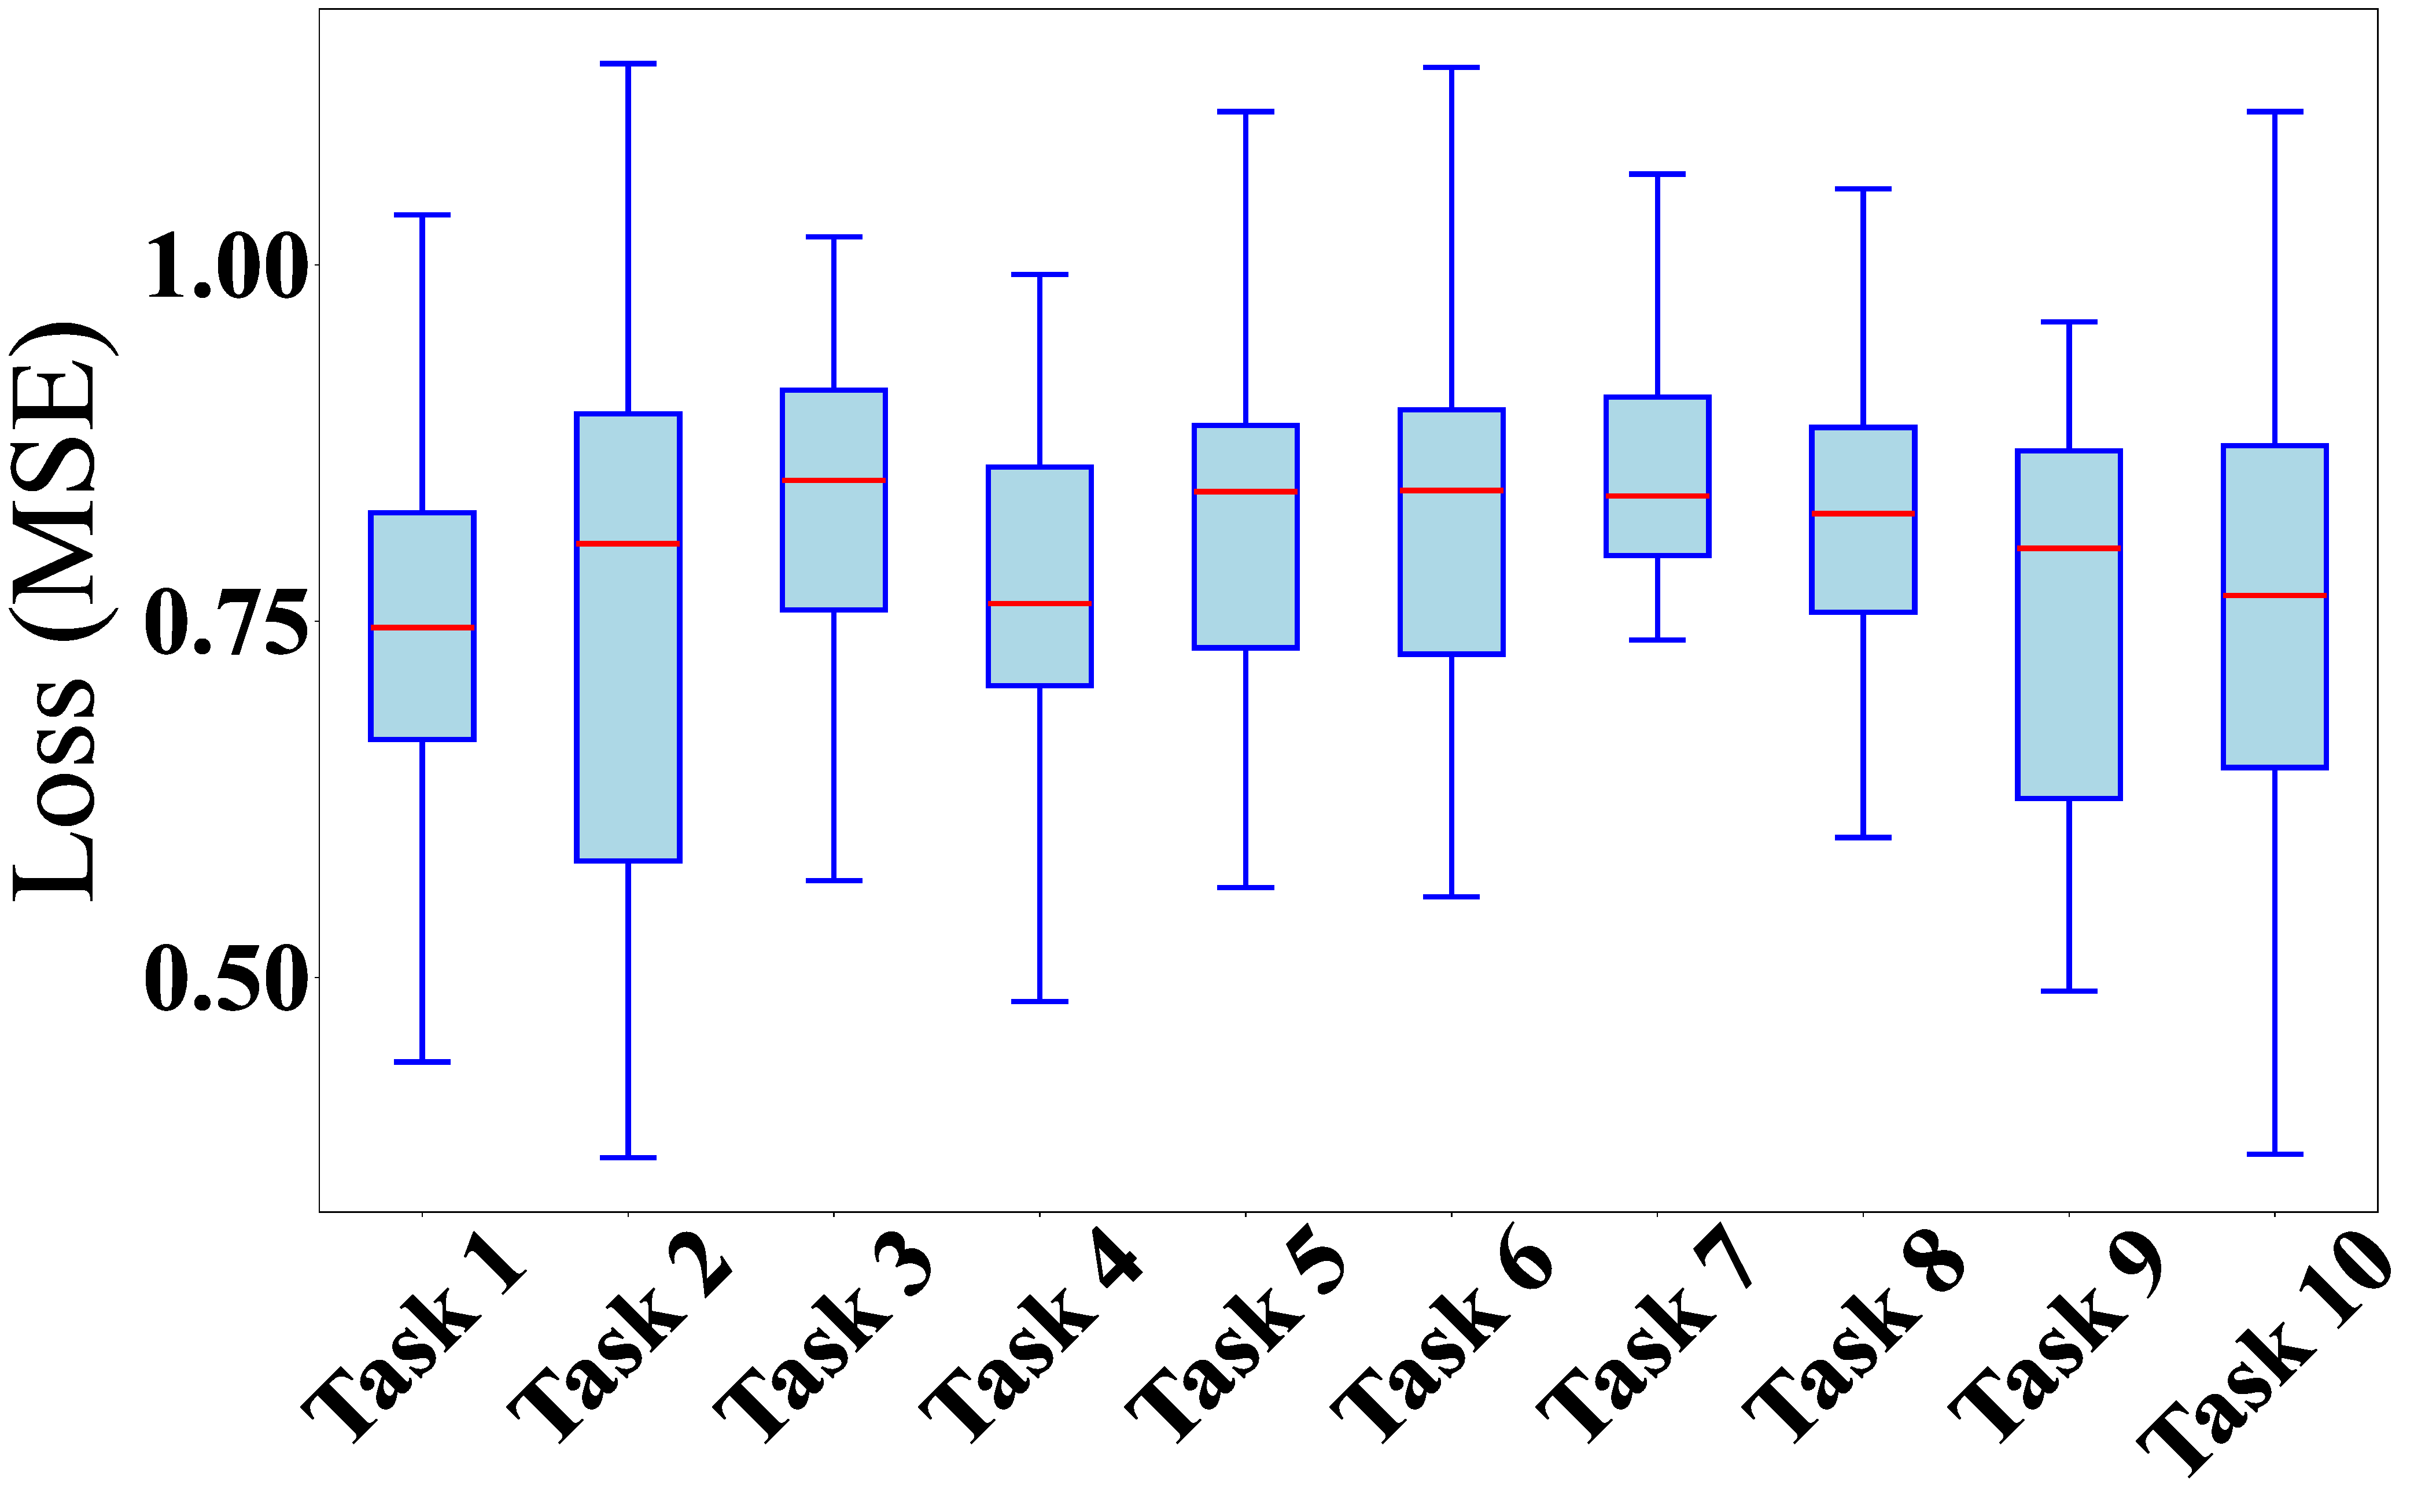
\includegraphics[width=\linewidth]{figures/box_plots/bcl_sine.pdf} \\
        \textbf{MER} &
        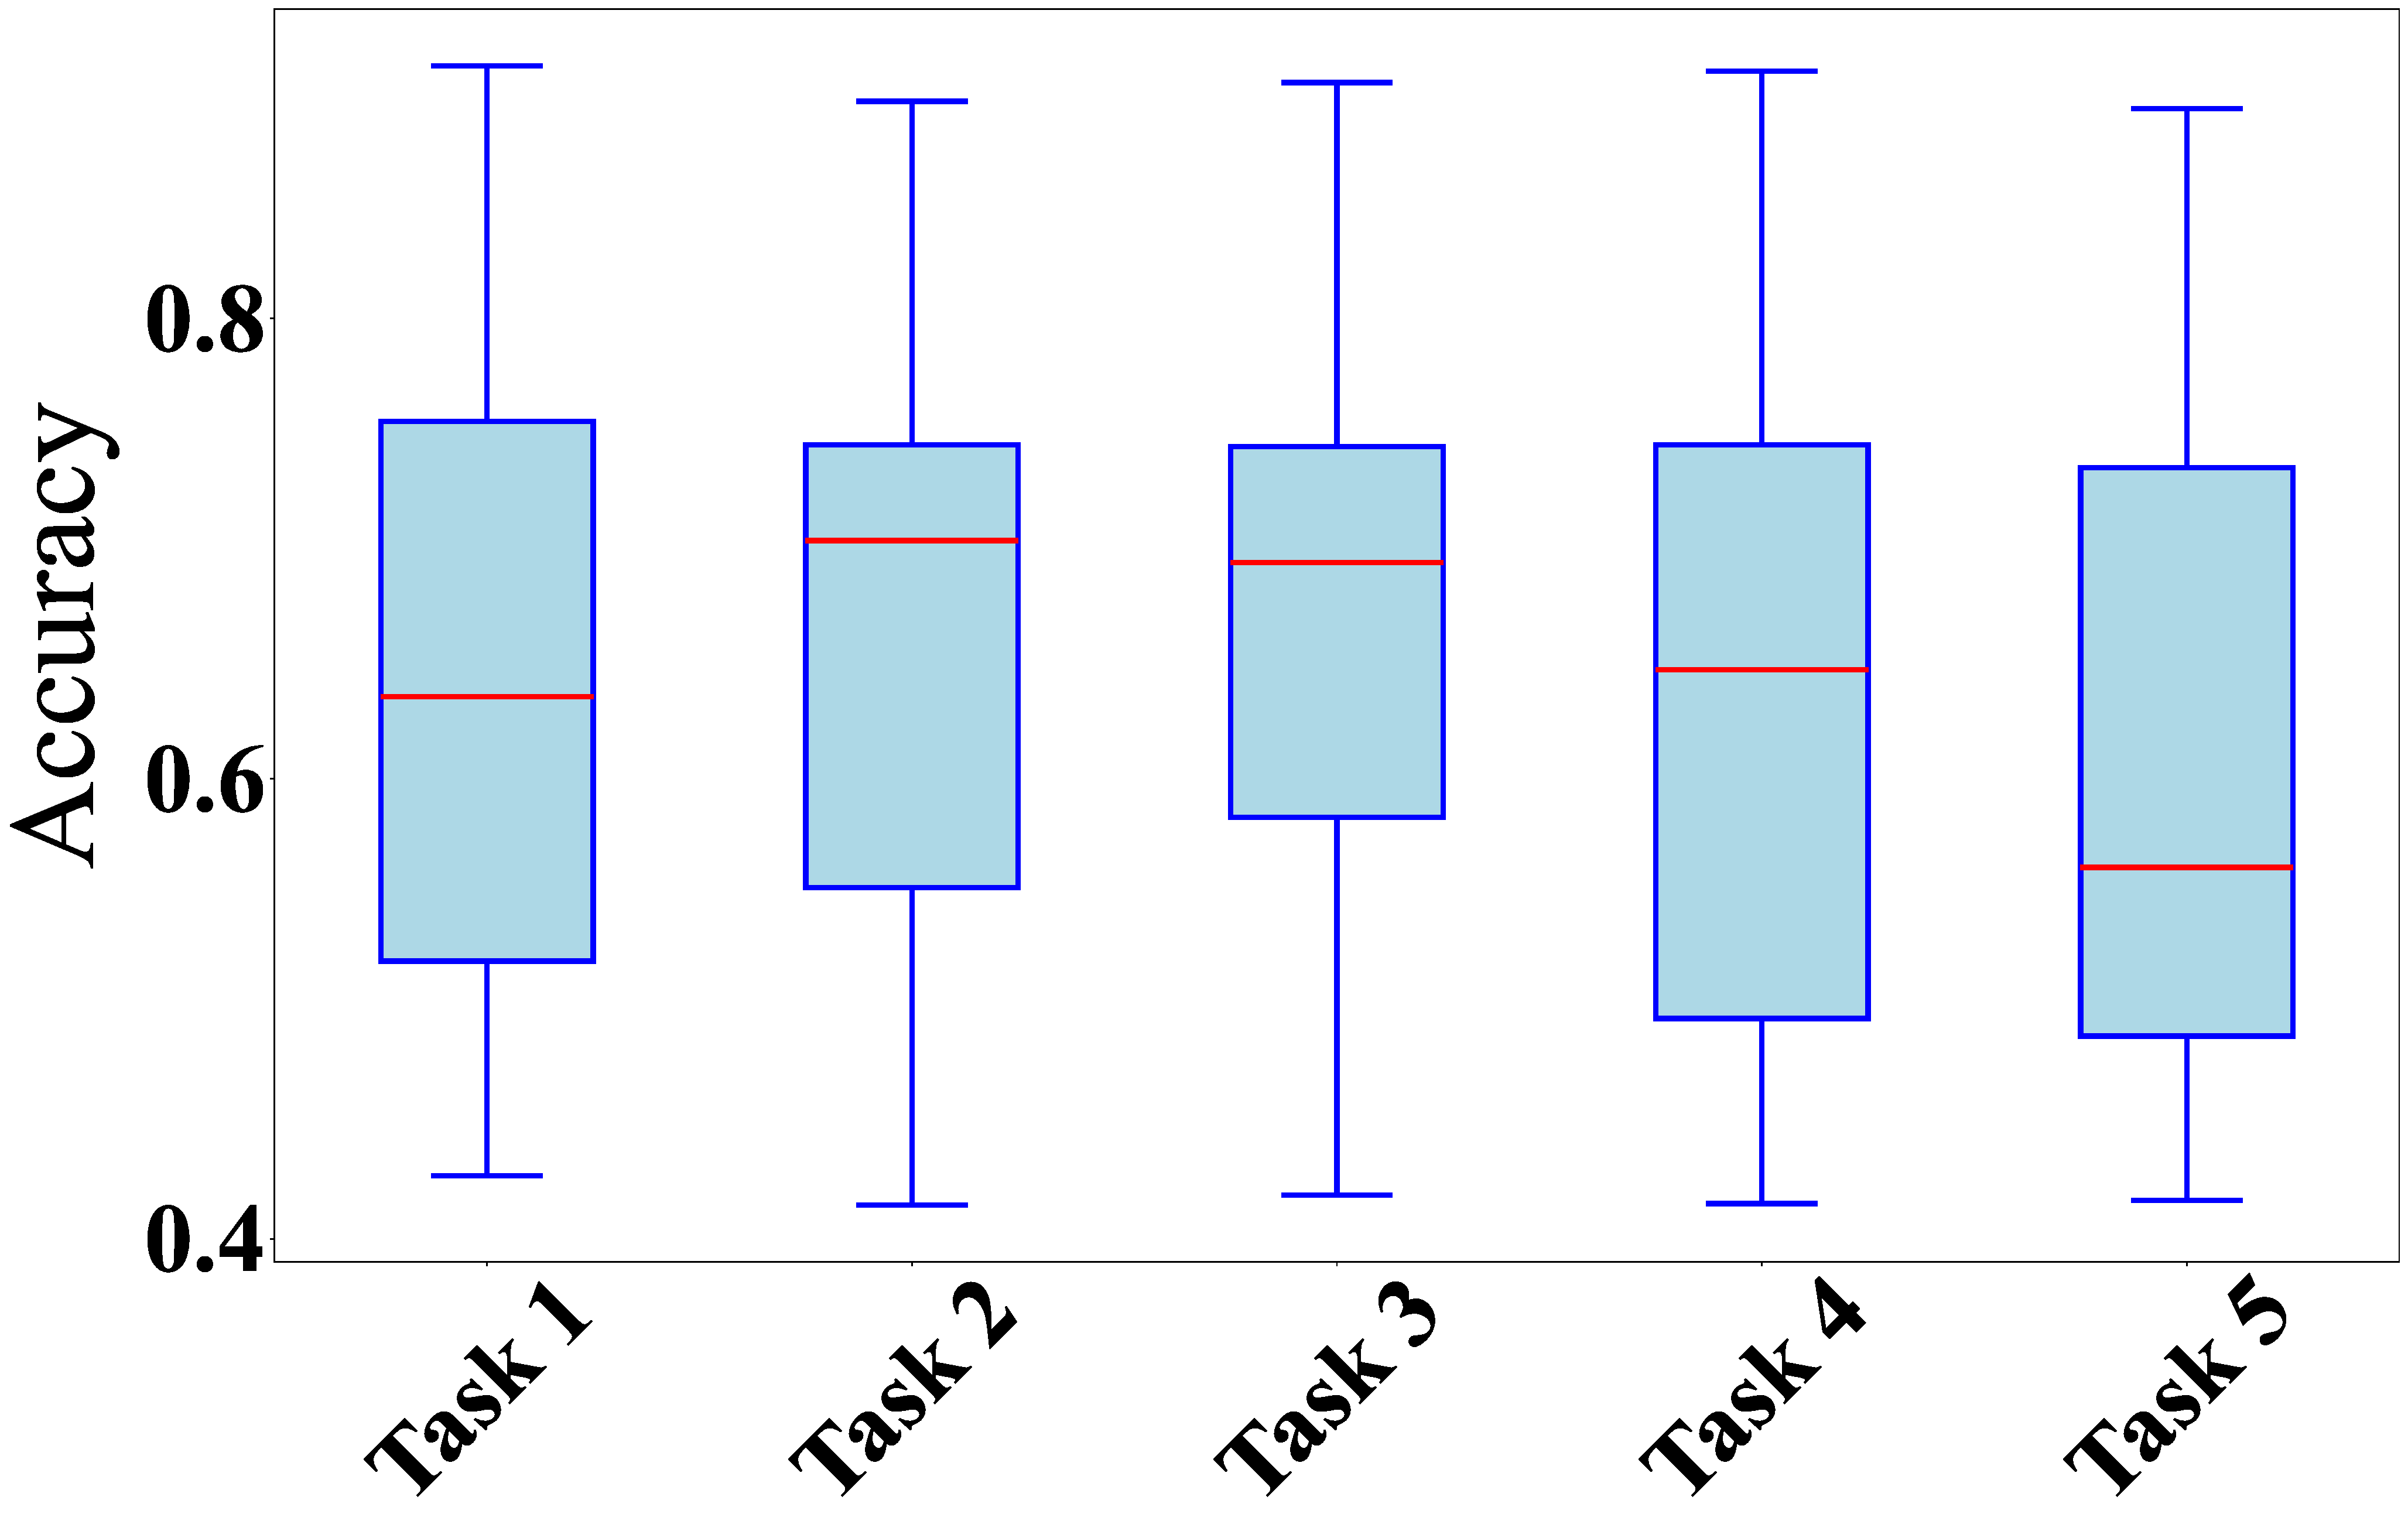
\includegraphics[width=\linewidth]{figures/box_plots/mer_image.pdf} &
        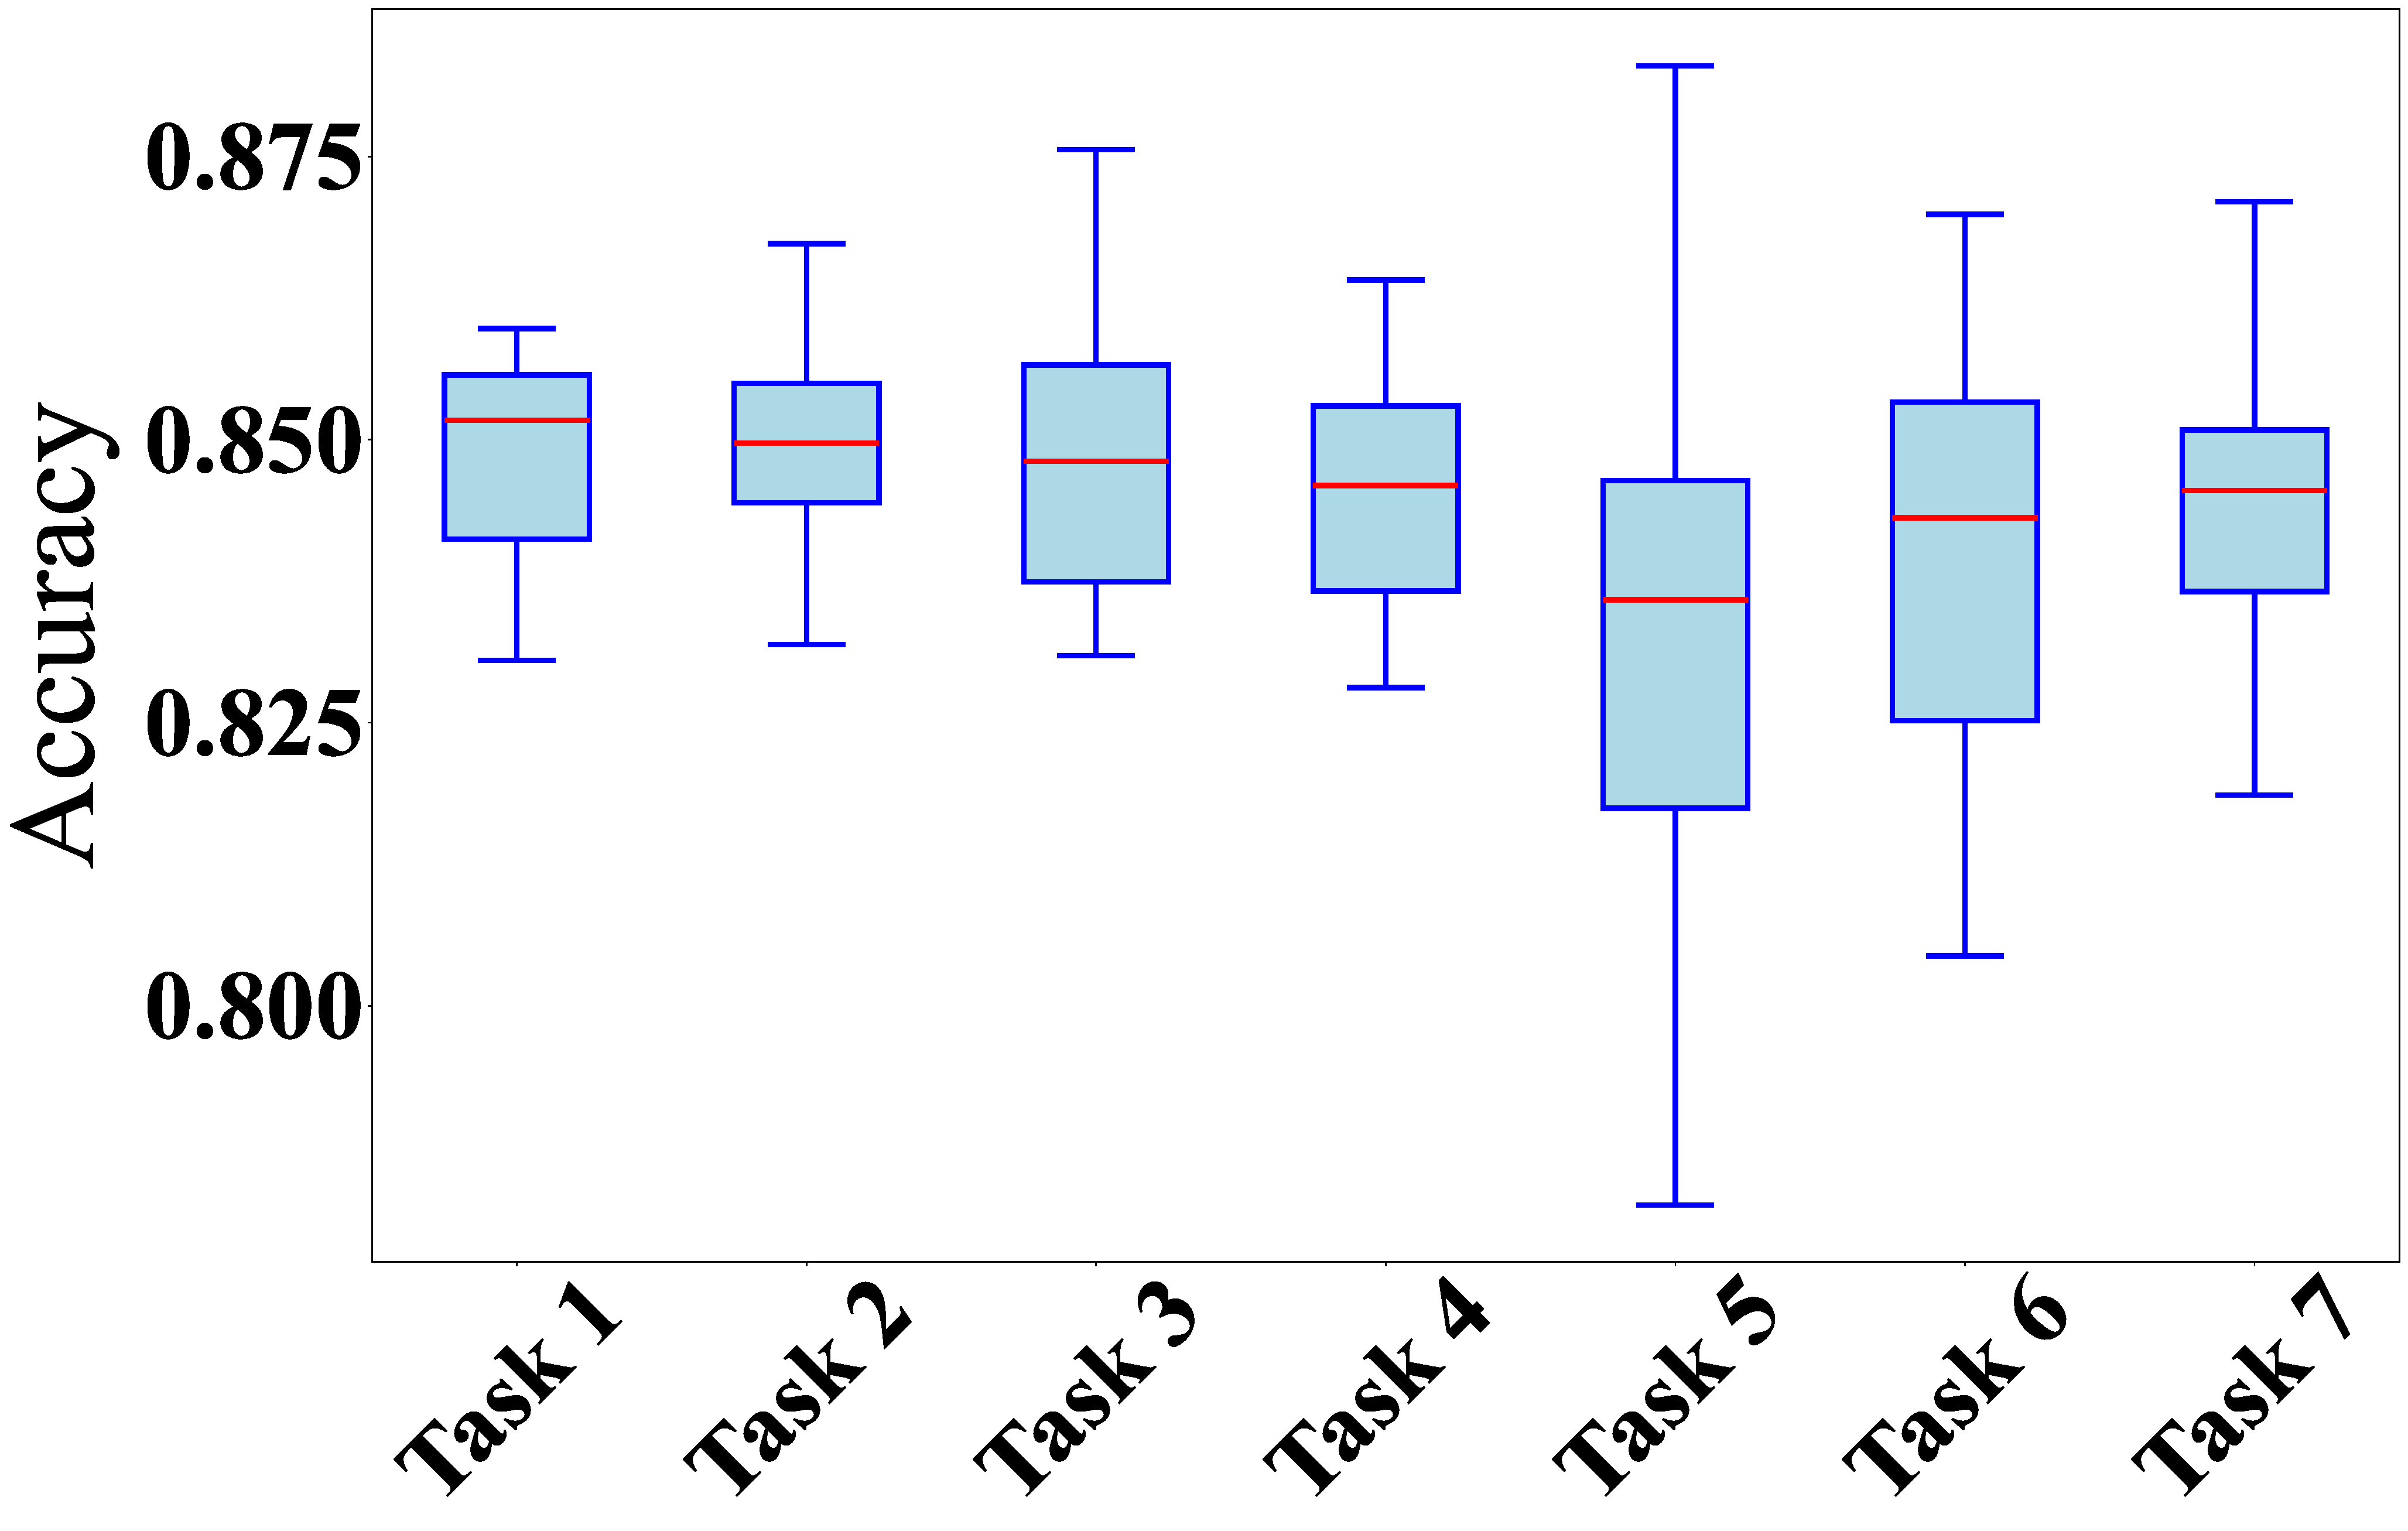
\includegraphics[width=\linewidth]{figures/box_plots/mer_text.pdf} &
        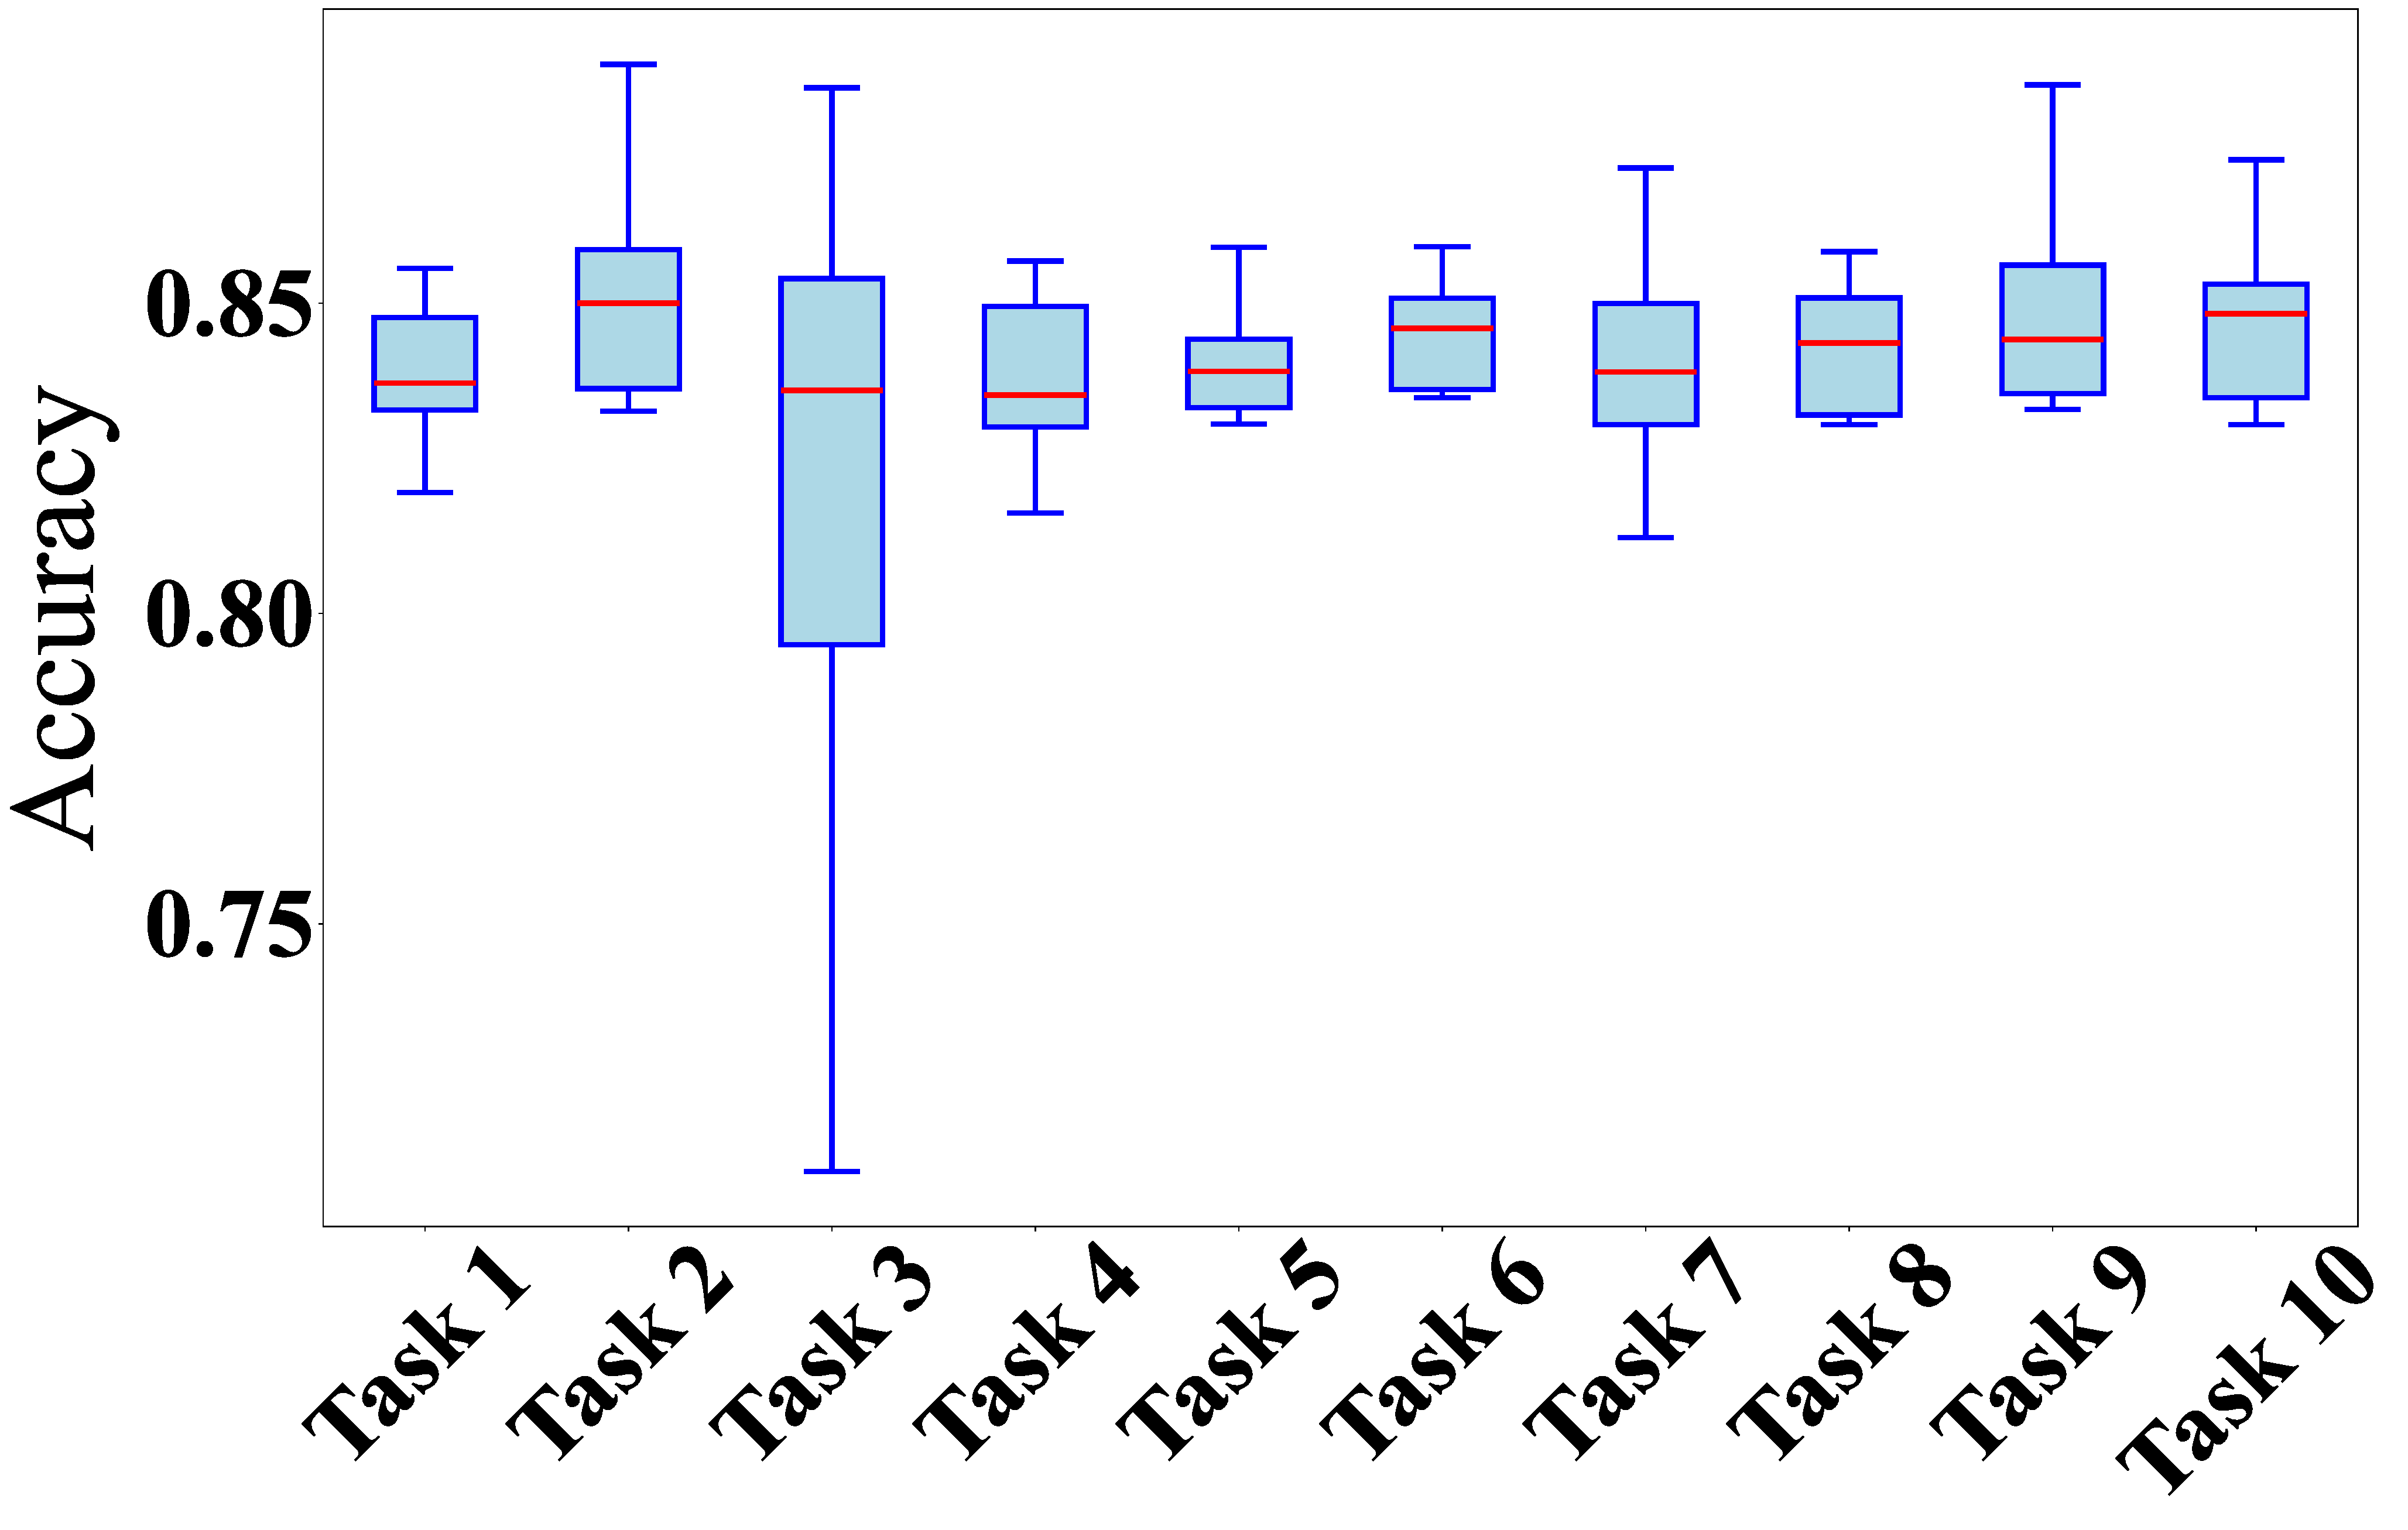
\includegraphics[width=\linewidth]{figures/box_plots/mer_graph.pdf} &
        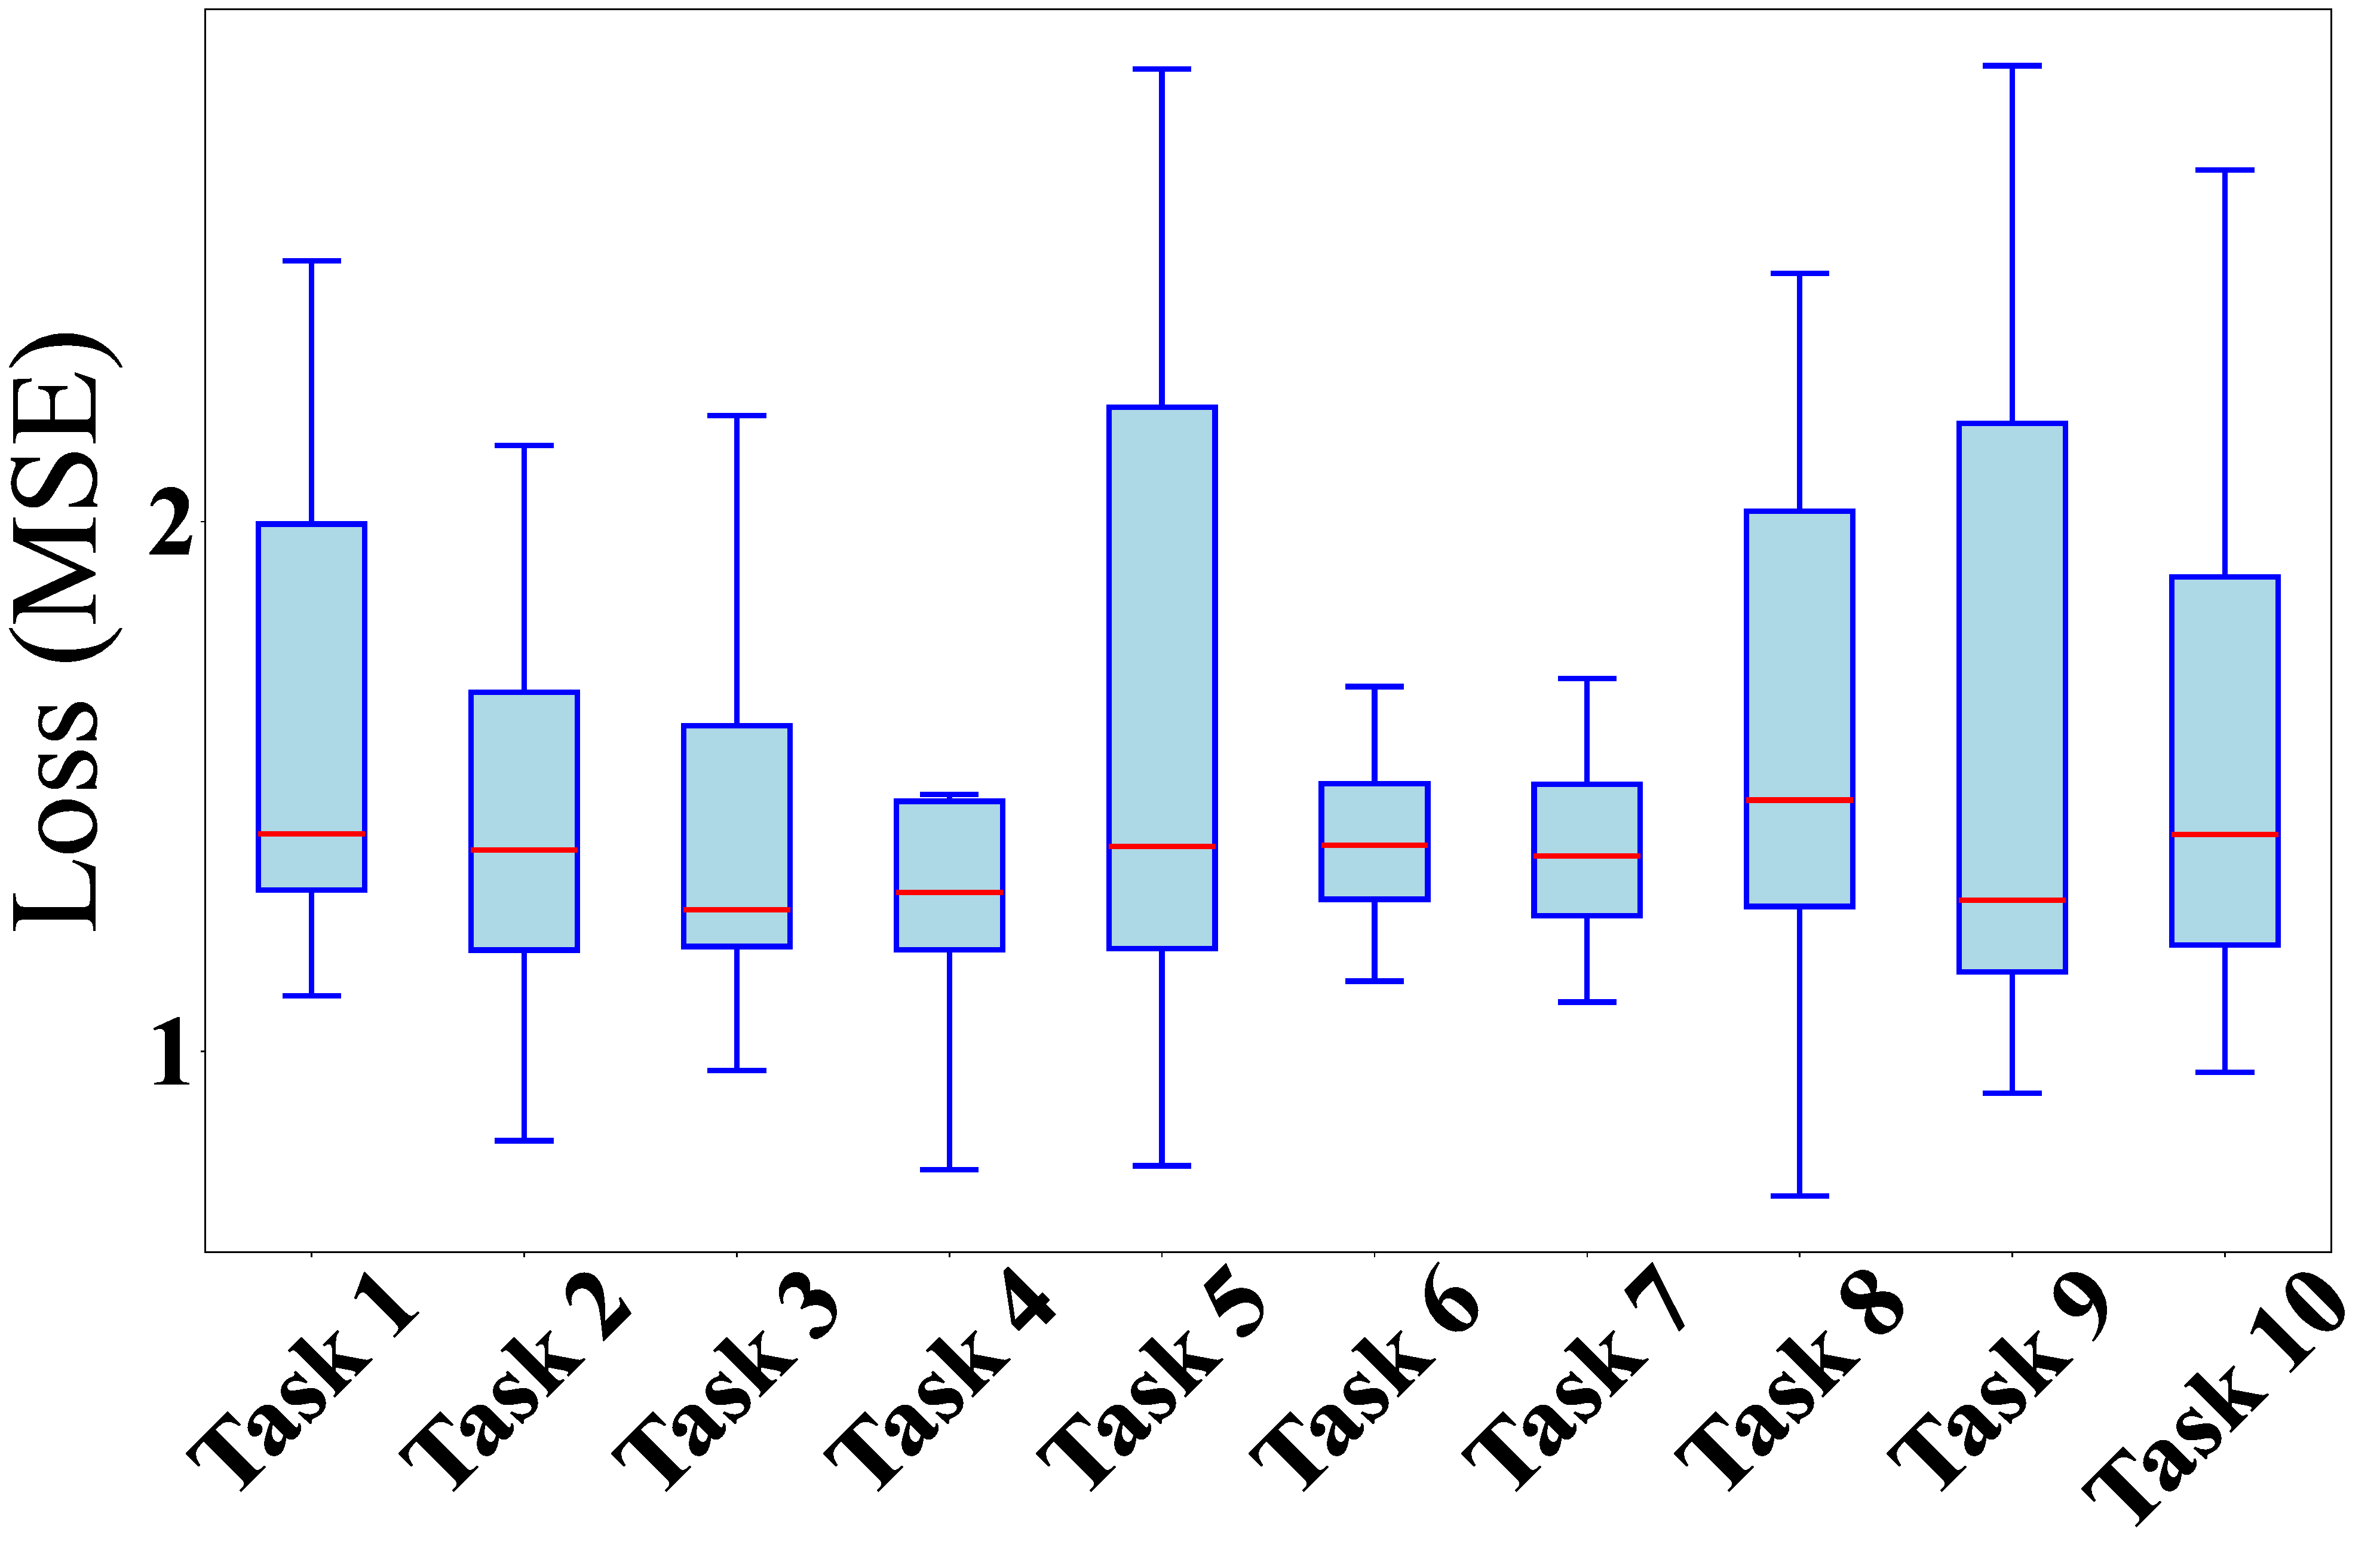
\includegraphics[width=\linewidth]{figures/box_plots/mer_sine.pdf} \\
    \end{tabular}%
    }
    \caption{Impact of task order comparison of CL methods—EWC, MER, BCL, and ER—across diverse domains, including image classification, text-based classification tasks, synthetic graph-structured data, and synthetic sine wave regression. The accuracies and mean squared error (MSE) losses shown are calculated after the model has learned all the tasks. Random task orders were generated for each method and domain, and the accuracy or loss was logged for each task in the sequence. The high variability observed in the box plots highlights the significant impact of task order on model performance in CL. This phenomenon is consistent across all evaluated domains.}
    \label{fig:results}
\end{figure*}

\subsection{Impact of Task Order Across Domains}
The box plots illustrate the variability in accuracy (or MSE loss) for each task across different sequences, highlighting the significant sensitivity of models to the task order.

To generate this plot, we randomly created 50 task sequences for each domain and logged the models' performance at each training stage. By training stage, we refer to the point at which a particular task is introduced to the model. While intermediate accuracy or loss values exhibited expected fluctuations, the final performance (after training on all tasks) demonstrates a striking dependency on the task order. To observe this, observe the size of the box plot corresponding to each task in each subplot in Fig.~\ref{fig:results}. Here,  the large interquartile range (IQR) underscores the extent of this variability that we hypothesize.

\textbf{Variability in Performance across Task Orders:}
Figure~\ref{fig:results} highlights the varying sensitivity of different CL methods to task ordering. This sensitivity is evident in the spread of the box plots, where methods with wider distributions exhibit higher variability in final accuracy (or loss), whereas methods with tighter distributions demonstrate more robustness to task order. %

We also note that the performance metrics can be disrupted by inconsistent sequencing. The IQR observed across methods and domains in Fig.~\ref{fig:results} reaffirms that task order is not merely a peripheral concern but a fundamental challenge in CL. Most approaches across different datasets struggle with sequence dependencies, suggesting the need for explicit task ordering strategies to enhance stability. While the range of variation is method-dependent, the range is extensive, with the minimum across all domains and methods being 2\% and the maximum being 22\%. Addressing this challenge requires domain-specific strategies to ensure consistency in learning outcomes. These insights further motivate the need for optimizing task sequencing strategies, as explored in the subsequent section, where we formalize the task ordering problem as an optimization challenge.

\section{Extended Results}
\label{app:extended-results}

\subsection{Evaluation Metrics}
\label{sec:metrics}

To rigorously assess the performance and stability of our framework, we employ three standard metrics commonly used in the CL literature. Let $A_{i, j}$ denote the test accuracy on task $j$ after the model has finished learning task $i$, and let $\ntasks$ be the total number of tasks. 

\textbf{Mean Accuracy.} We report the mean accuracy across all observed tasks after the training sequence is complete . It is defined as: 
\begin{equation}
    \text{Mean Accuracy} = \frac{1}{\ntasks} \sum_{j=1}^{\ntasks} A_{\ntasks, j}
\end{equation}

\textbf{Average Forgetting.} To quantify the extent of catastrophic forgetting, we measure the average decrease in performance for each task from its peak accuracy (immediately after training on that task) to its final accuracy \cite{yoon2019scalable}. This is calculated as: 
\begin{equation}
    \text{Avg. Forgetting} = \frac{1}{\ntasks-1} \sum_{j=1}^{\ntasks-1} \max_{l \in \{1, \dots, \ntasks-1\}} (A_{l,j} - A_{\ntasks,j})
\end{equation}

\textbf{Standard Deviation.} To evaluate robustness against random task orderings, we report the standard deviation of the final average accuracy across all evaluated permutations ~\cite{bell2022effect}. For a set of $P$ permutations, this is given by:
\begin{equation}
    \sigma_{\text{perm}} = \sqrt{\frac{1}{P} \sum_{p=1}^{P} (\text{ACC}_p - \mu_{\text{ACC}})^2}
\end{equation}

where $\text{ACC}_p$ is the Average Accuracy for the $p$-th permutation and $\mu_{\text{ACC}}$ is the mean over all permutations. A lower $\sigma_{\text{perm}}$ indicates a method that is less sensitive to the specific order in which tasks arrive.

\subsection{Detailed Setup}
\label{sec:detailed_setup}

We evaluate our approach on five diverse continual learning
benchmarks spanning image classification, text classification, and graph
node classification. Each dataset is partitioned into disjoint tasks
following the domain-incremental or class-incremental learning protocol, where each task introduces a new subset of classes not seen in previous tasks.
Table~\ref{tab:dataset_setup} summarizes the dataset configurations and Table~\ref{tab:architectures} the per-dataset
architectures.

\begin{table*}[!htbp]
\centering
\caption{Dataset configurations for continual learning experiments. Each dataset is split into sequential tasks with disjoint class subsets. Labels are remapped to $\{0, \ldots, C_t-1\}$ within each task.}
\label{tab:dataset_setup}
\resizebox{\textwidth}{!}{%
\begin{tabular}{lcccccc}
\toprule
\textbf{Dataset} & \textbf{Total Classes} & \textbf{Tasks} & \textbf{Classes/Task} & \textbf{Input Dim.} & \textbf{Buffer Size} & \textbf{Domain} \\
\midrule
Split-MNIST      & 10  & 5  & 2  & $28 \times 28 \times 1$   & 50  & Image \\
CIFAR-100        & 100 & 10 & 10 & $32 \times 32 \times 3$   & 500 & Image \\
20 Newsgroups    & 20  & 5  & 4  & 20{,}000 (TF-IDF)         & 100 & Text  \\
Cora             & 7   & 3  & 2--3 & 1{,}433 (node features) & 50  & Graph \\
ImageNet-100 & 100 & 10 & 10 & $224 \times 224 \times 3$ & 500 & Image (ViT) \\
\bottomrule
\end{tabular}%
}
\end{table*}

\begin{table*}[!htbp]
\centering
\caption{Per-dataset architectures. The same backbone is used for the local learner and every level of the hierarchical model.}
\label{tab:architectures}

\renewcommand{\arraystretch}{1.45}
\setlength{\tabcolsep}{7pt}
\definecolor{rowgray}{HTML}{F4F6F9}
\arrayrulecolor{black!75}

\rowcolors{2}{rowgray}{white}
\begin{tabularx}{\linewidth}{@{} l l l X @{}}
\toprule
\textbf{Dataset} & \textbf{Backbone} & \textbf{Input} & \textbf{Layer pipeline} \\
\midrule
Split-MNIST   & CNN + ResNet-18 & $1{\times}28{\times}28$ &
  Conv$(1{\to}64)$ $\to$ MaxPool $\to$ Conv$(64{\to}128)$ $\to$ MaxPool
  $\to$ $1{\times}1$ proj$(128{\to}3)$ $\to$ ResNet-18 $\to$
  Linear$(512{\to}2)$ \\
CIFAR-100     & ResNet-18       & $3{\times}32{\times}32$ &
  ResNet-18 with first conv replaced by $3{\times}3$, stride $1$,
  no maxpool $\to$ Linear$(512{\to}10)$ \\
Cora          & 2-layer GCN     & 1{,}433-dim node features &
  GCNConv$(1433{\to}128)$ $\to$ ReLU $\to$ Dropout$(0.5)$ $\to$
  GCNConv$(128{\to}128)$ $\to$ ReLU $\to$ Dropout$(0.5)$ $\to$
  Linear$(128{\to}3)$ \\
20 Newsgroups & 3-layer MLP     & 20{,}000-dim TF-IDF &
  Linear$(20000{\to}1024)$ $\to$ ReLU $\to$ Dropout$(0.5)$ $\to$
  Linear$(1024{\to}512)$ $\to$ ReLU $\to$ Dropout$(0.5)$ $\to$
  Linear$(512{\to}4)$ \\
ImageNet-100  & ViT-S/16        & $3{\times}224{\times}224$ &
  Pretrained ViT-S/16 from \texttt{timm} (12 layers, 6 heads, hidden
  $384$, patch $16$; ${\approx}21.7$M params) $\to$
  Linear$(384{\to}10)$ \\
\bottomrule
\end{tabularx}
\end{table*}

\paragraph{Image Classification.}
For \textbf{Split-MNIST}, we partition the 10 digit classes into 5 consecutive tasks, each containing 2 classes (e.g., Task 1: digits 0--1, Task 2: digits 2--3, etc.). The grayscale images ($28 \times 28$) are normalized and fed directly to the network. Because ResNet-18 expects a 3-channel input, the leading 2-layer CNN lifts the single-channel image to a 3-channel representation before the backbone. For \textbf{CIFAR-100}, we divide the 100 fine-grained classes into 10 tasks of 10 classes each. We apply standard data augmentation including random crops with 4-pixel padding and horizontal flips during training. The first convolution of ResNet-18 is replaced with a $3\!\times\!3$ stride-$1$ layer and the initial maxpool is removed so that the $32 \times 32$ input is not down-sampled too aggressively.

\paragraph{Image Classification at Scale (ImageNet-100).}
To verify that HTCL transfers to large-scale, modern transformer architectures, we additionally evaluate on a 100-class subset of ImageNet. The $100$ classes are partitioned into $10$ tasks of $10$ classes each. Images are resized to $224\!\times\!224$, normalized with the standard ImageNet mean and standard deviation, and augmented at training time with random resized crops and horizontal flips. The backbone is a ViT-S/16 ($\approx\!21.7$M parameters) initialized from the publicly available \texttt{timm} weights and finetuned end-to-end. Following the domain-incremental protocol described above, the classifier head is a single linear layer mapping the $384$-dimensional ViT features to the
$10$ task-local classes; per-task labels are remapped to $\{0, \ldots, 9\}$ as in the other benchmarks. 

\paragraph{Text Classification.}
The \textbf{20 Newsgroups} dataset consists of approximately 18,000 newsgroup posts across 20 categories. We extract TF-IDF features with a vocabulary size of 20,000 and partition the categories into 5 tasks of 4 classes each. The features are consumed by a 3-layer MLP with two hidden ReLU blocks of width $1024$ and $512$, each followed by dropout at rate $0.5$.

\paragraph{Graph Classification.}
For \textbf{Cora}, a citation network with 2,708 nodes and 7 classes, we split the classes into 3 tasks. Nodes are randomly partitioned into 80\% training and 20\% test sets while preserving class distributions. We use the 1,433-dimensional bag-of-words node features as input. The classifier is a 2-layer Graph Convolutional Network with hidden width $128$ and dropout $0.5$ between layers, operating on the full graph at every forward pass so that the message-passing structure is preserved across tasks.

\paragraph{Training Protocol.}
All experiments use SGD with momentum 0.9. Table~\ref{tab:hyperparams} details the hyperparameter settings. For replay-based methods (ER, DER, SER, and HTCL), we maintain an experience replay buffer that stores samples from previous tasks. The buffer is populated using reservoir sampling to ensure balanced representation across all seen classes. On ImageNet-100 the same SGD configuration is used with the lower learning rate of $10^{-3}$ that is standard for finetuning ViTs from pretrained weights.

\begin{table*}[ht]
\centering
\caption{Training hyperparameters for each dataset.}
\label{tab:hyperparams}
\begin{tabular}{lccccc}
\toprule
\textbf{Parameter} & \textbf{ImageNet-100} & \textbf{Split-MNIST} & \textbf{CIFAR-100} & \textbf{20 Newsgroups} & \textbf{Cora} \\
\midrule
Learning Rate      & $10^{-3}$ & 0.01      & 0.1       & 0.001     & 0.01  \\
Batch Size         & 32       & 64        & 32        & 32        & 32    \\
Epochs per Task    & 5         & 10        & 10        & 10        & 10    \\
Weight Decay       & $10^{-4}$ & $10^{-4}$ & $10^{-4}$ & $10^{-4}$ & $10^{-4}$ \\
Buffer Size        & 500      & 50        & 500       & 100       & 50    \\
\bottomrule
\end{tabular}
\end{table*}

\paragraph{HTCL-Specific Parameters.}
For our hierarchical approach, we evaluate configurations with $\nlev \in \{2, 3\}$ hierarchy levels. The group size is set to $\gsize=2$ tasks per group. We regularization strength $\reg > -\mu_{\min}(\mathbf{H}^{(t-1)})$. 

All experiments are conducted on a single NVIDIA GPU with CUDA 12.3. We report results averaged over 200 random task orderings to account for permutation sensitivity, with standard deviations included. The random seed is fixed at 42 for reproducibility.

\subsection{Finding the Optimal Group Size}
\label{app:break-even-point}

{Increasing the group size $k$ allows HTCL to explore a larger space of intra-group orderings. However, this benefit comes at a factorial computational cost, as the number of permutations scales as $k!$, while the achievable accuracy is inherently bounded by the optimal task order (see Theorem~\ref{prop:group_vs_random}). The key question is therefore where the additional compute ceases to yield meaningful gains.

To study this trade-off on SplitMNIST with SER + HTCL-L2, we sweep $k \in \{1, \dots, 5\}$ and measure the marginal accuracy gain normalized by the logarithmic increase in compute:
\begin{equation}
    \rho(k \to k{+}1)
    \;=\;
    \frac{\mathrm{acc}(k{+}1) - \mathrm{acc}(k)}{\log_{10} time(k{+}1) - \log_{10} time(k)},
    \label{eq:break_even_metric}
\end{equation}
where $time(k)$ denotes the wall-clock time at group size $k$.

As shown in Fig.~\ref{fig:break-even-point}, $\rho$ increases from $k=1 \to 2$ and peaks at $k=2 \to 3$, after which it drops sharply and approaches zero. This indicates a clear point of diminishing returns: beyond $k=3$, additional compute yields negligible accuracy improvements. 

While the exact location of this "break-even point" may vary across benchmarks, its presence is expected, since factorial growth in compute will eventually dominate any bounded accuracy gains.

\begin{figure}[!t]
  \centering
  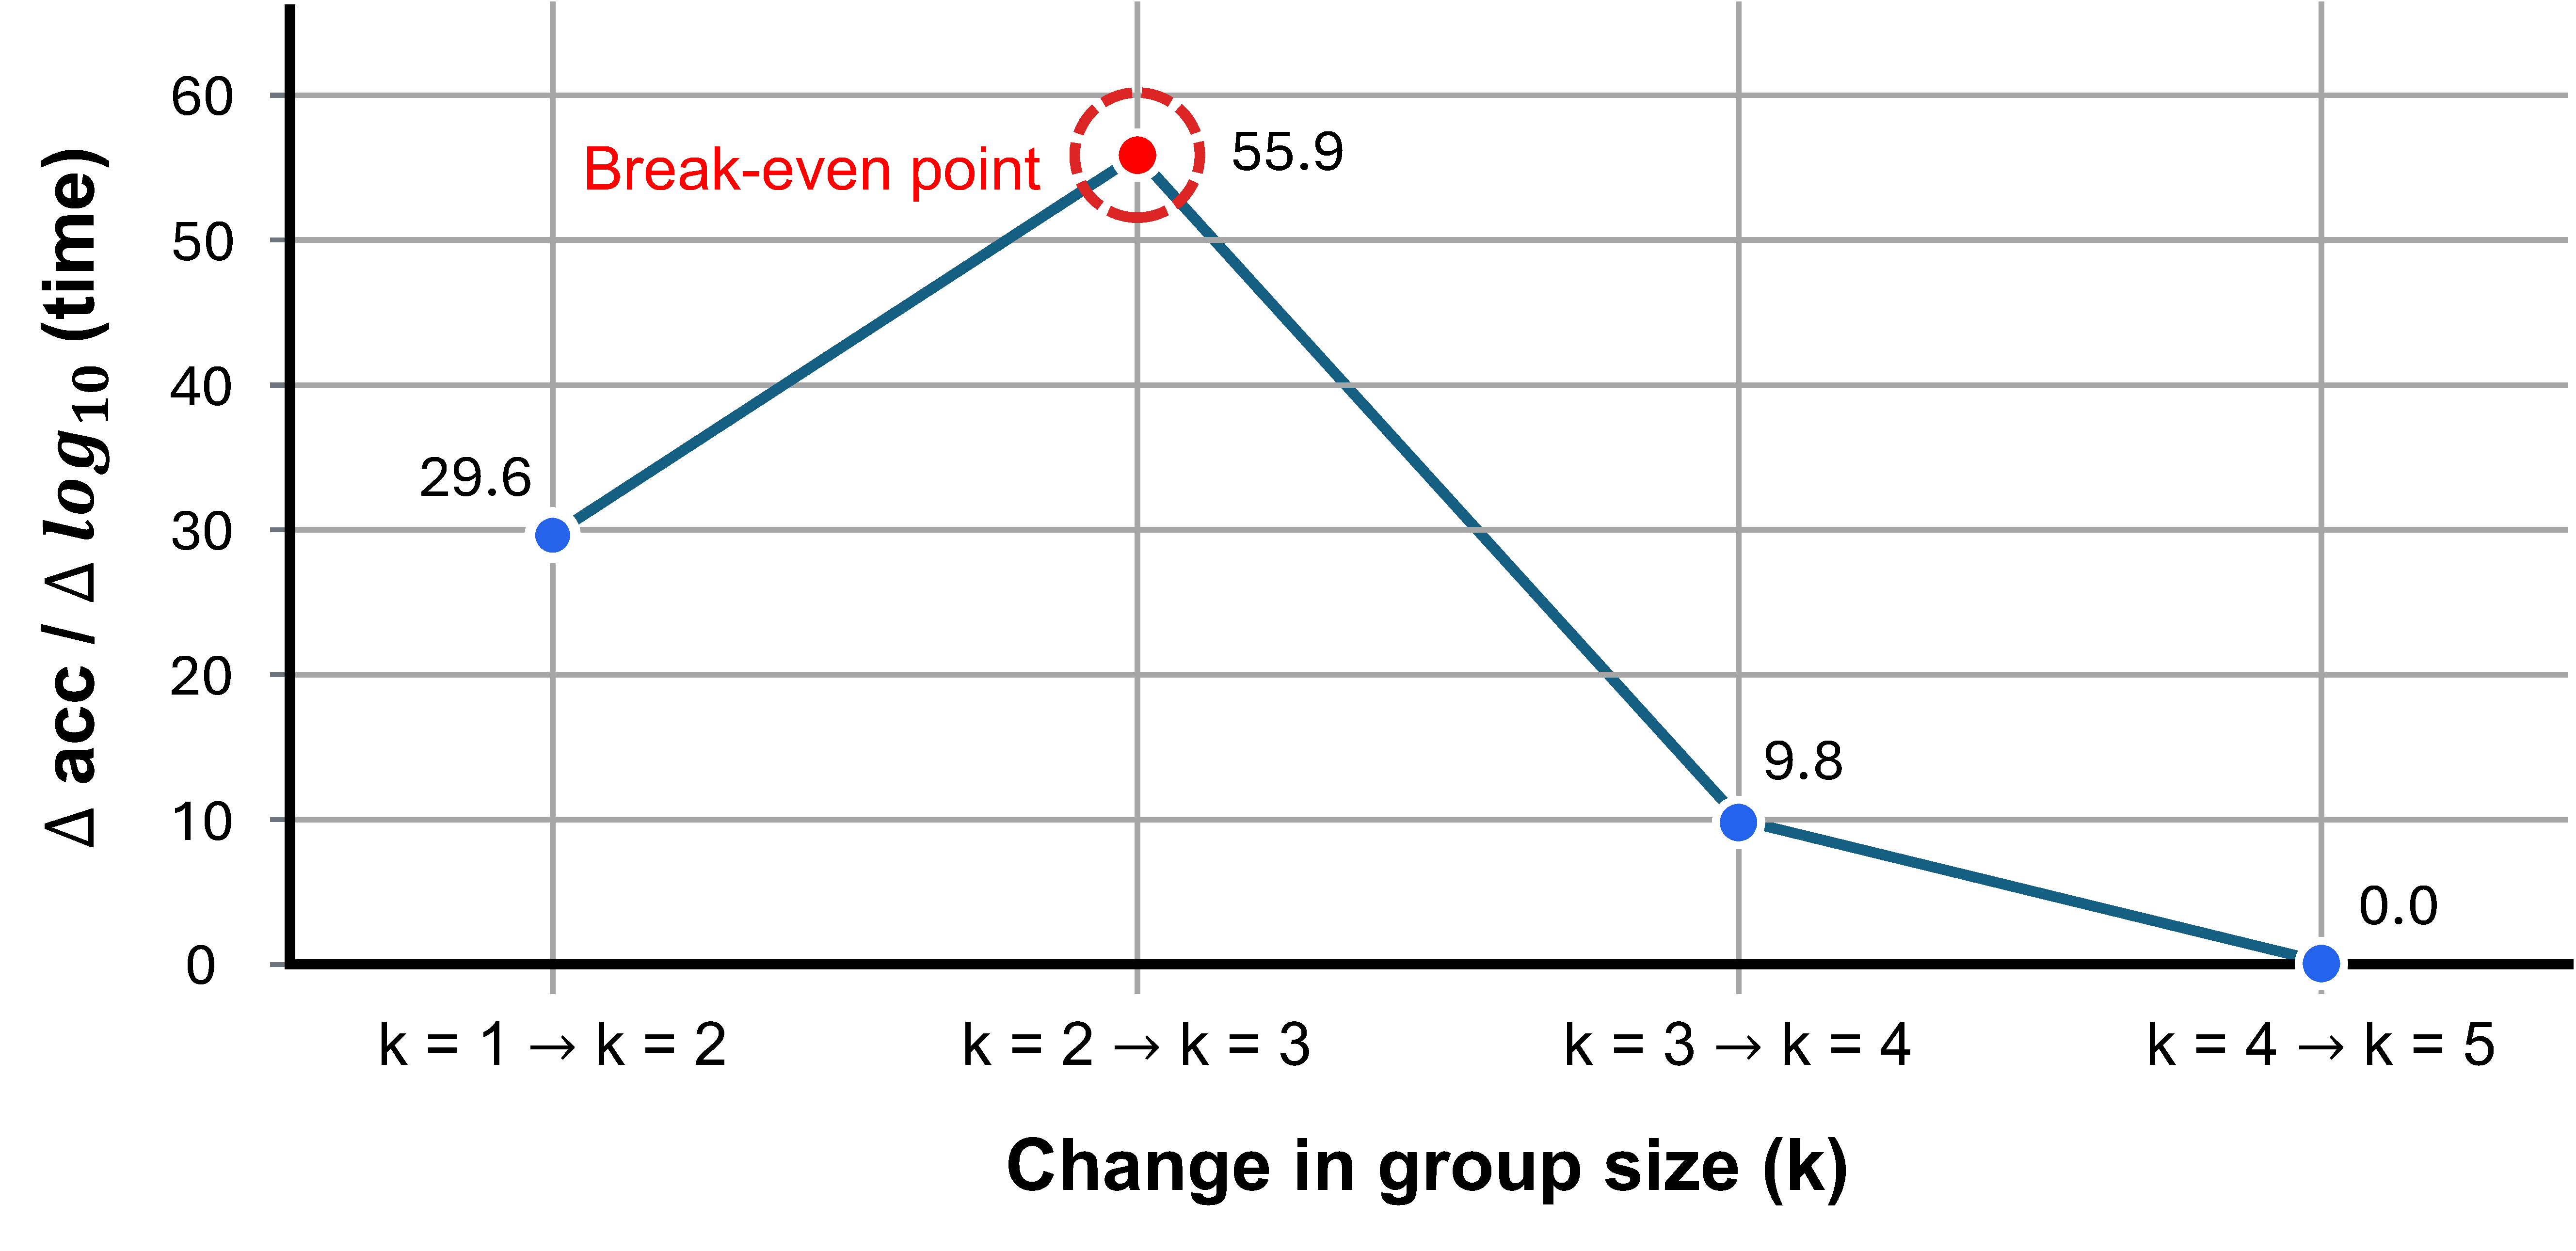
\includegraphics[width=\columnwidth]{figures/optimal-group-size/knee.pdf}
  \caption{\textbf{Break-even point in group size on SplitMNIST
    (SER + HTCL-L2).} The marginal return $\rho$ from
    Eq.~\eqref{eq:break_even_metric} climbs from $29.6$ at $k=1 \to 2$
    to a peak of $55.9$ at $k=2 \to 3$, then collapses to $9.8$ at
    $k=3 \to 4$ and to $\approx 0$ at $k=4 \to 5$. Beyond the peak,
    every additional ten times of compute buys essentially no accuracy.}
    \label{fig:break-even-point}
\end{figure}

\subsection{Comparison with First-order Consolidation and DiLoCo-style Aggregator}
\label{app:fo-diloco}

We examine the role of the diagonal Hessian in Eq.~\eqref{eq:hier_update-main} from two complementary perspectives.

\textbf{Internal ablation.} Setting $\mathbf{H}^{(t-1)} = \mathbf{0}$ reduces the preconditioner to $(\reg \mathbf{I})^{-1} = \reg^{-1}\mathbf{I}$, yielding the first-order proximal update
\begin{equation}
\label{eq:firstorder}
\begin{aligned}
\whT{1}{t} &= \whT{1}{t-1} + \frac{1}{\reg}\!\left(\reg\,\Dd^{(t)} - \mathbf{g}^{(t-1)}\right) \\
&= \whT{1}{t-1} + \Dd^{(t)} - \frac{1}{\reg}\mathbf{g}^{(t-1)}.
\end{aligned}
\end{equation}
This form preserves the proximal term $\Dd^{(t)}$ and the gradient correction $\mathbf{g}^{(t-1)}/\reg$, but removes curvature information.

\textbf{External comparison.} HTCL follows a group-wise train-then-consolidate procedure that is structurally similar to DiLoCo's outer-update framework~\cite{douillard2023diloco}, where multiple workers train independently and their models are periodically aggregated. The two approaches differ in how this aggregation is performed. DiLoCo uses first-order parameter averaging across workers, while HTCL applies a second-order Taylor update using the diagonal Hessian as a preconditioner. To isolate this difference, we construct a DiLoCo-style variant by replacing $\whT{1}{t}$ with the elementwise mean of the $K$ worker models at each group boundary, keeping all other components unchanged. Both variants are evaluated on SplitMNIST with $k = 2$ and $L = 2$. Results are reported in Table~\ref{tab:firstorder}.

\begin{table}[!htbp]
\centering
\caption{First-order consolidation variants on SplitMNIST with $k = 2$, $L = 2$. Accuracy, standard deviation, and forgetting are reported in \%. Arrows indicate the direction of change relative to the standalone baseline. The best value per metric within each baseline group is bolded.}
\label{tab:firstorder}
\small
\setlength{\tabcolsep}{6pt}
\renewcommand{\arraystretch}{1.05}
\begin{tabular}{lccc}
\toprule
Method & Accuracy & Std & Forgetting \\
\midrule
ER                                & 89.3              & \phantom{0}5.5              & 30.3 \\
ER + HTCL-L2                      & \textbf{92.0} $\uparrow$ & \phantom{0}\textbf{3.5} $\downarrow$ & \textbf{12.5} $\downarrow$ \\
ER + HTCL$_{\text{1st}}$          & 60.5 $\downarrow$ & 10.9 $\uparrow$            & 20.2 $\downarrow$ \\
ER + DiLoCo                       & 70.5 $\downarrow$ & \phantom{0}8.3 $\uparrow$  & 14.1 $\downarrow$ \\
\midrule
SER                               & 88.5              & \phantom{0}5.6              & 32.0 \\
SER + HTCL-L2                     & \textbf{95.6} $\uparrow$ & \phantom{0}\textbf{1.8} $\downarrow$ & \phantom{0}9.8 $\downarrow$ \\
SER + HTCL$_{\text{1st}}$         & 67.5 $\downarrow$ & 12.4 $\uparrow$            & 12.1 $\downarrow$ \\
SER + DiLoCo                      & 67.0 $\downarrow$ & \phantom{0}6.8 $\uparrow$  & \phantom{0}\textbf{9.4} $\downarrow$ \\
\midrule
DER                               & 86.5              & \phantom{0}4.9              & 35.0 \\
DER + HTCL-L2                     & \textbf{95.1} $\uparrow$ & \phantom{0}\textbf{1.8} $\downarrow$ & \textbf{10.2} $\downarrow$ \\
DER + HTCL$_{\text{1st}}$         & 68.1 $\downarrow$ & 11.4 $\uparrow$            & 11.1 $\downarrow$ \\
DER + DiLoCo                      & 71.2 $\downarrow$ & \phantom{0}5.5 $\uparrow$  & 15.3 $\downarrow$ \\
\midrule
EWC                               & 79.3              & \phantom{0}9.8              & 42.8 \\
EWC + HTCL-L2                     & \textbf{85.2} $\uparrow$ & \phantom{0}\textbf{6.2} $\downarrow$ & 28.9 $\downarrow$ \\
EWC + HTCL$_{\text{1st}}$         & 63.0 $\downarrow$ & 14.2 $\uparrow$            & \textbf{21.9} $\downarrow$ \\
EWC + DiLoCo                      & 59.1 $\downarrow$ & 18.7 $\uparrow$            & 29.1 $\downarrow$ \\
\midrule
SR                                & 88.0              & \phantom{0}7.5              & 31.0 \\
SR + HTCL-L2                      & \textbf{90.0} $\uparrow$ & \phantom{0}\textbf{5.0} $\downarrow$ & 14.0 $\downarrow$ \\
SR + HTCL$_{\text{1st}}$          & 61.4 $\downarrow$ & 11.9 $\uparrow$            & 16.5 $\downarrow$ \\
SR + DiLoCo                       & 68.8 $\downarrow$ & \phantom{0}7.8 $\uparrow$  & \textbf{11.5} $\downarrow$ \\
\bottomrule
\end{tabular}
\end{table}

Across all baselines, both first-order variants reduce forgetting but consistently lower accuracy relative to the standalone models. They also increase variability across task orderings, as reflected in higher standard deviations. In contrast, the second-order update (HTCL-L2) improves both accuracy and stability while reducing forgetting.

These results indicate that the diagonal Hessian plays a central role in the consolidation step. Removing it—either by zeroing $\mathbf{H}^{(t-1)}$ or by replacing the update with parameter averaging—changes the balance between stability and accuracy and increases sensitivity to task ordering.

\subsection{Experiments on Large Scale Dataset: ImageNet-100 with ViT Architecture}
\label{app:large-scale}

To stress HTCL beyond small-scale benchmarks, we evaluate on a 100-class ImageNet subset (10 sequential tasks, 10 classes per task) with a ViT-S/16 backbone. Both domain-incremental and class-incremental protocols are reported, with $k = 2$, $L = 2$, and 200 task permutations per setting. Training matches the prior protocol (5 epochs per task, AdamW, batch 32, replay buffer 500). Results appear in Table~\ref{tab:imagenet100}.

\begin{table}[!htbp]
\centering
\caption{ImageNet-100 with ViT-S/16, $k = 2$, $L = 2$, 200 task permutations per setting. Accuracy, standard deviation, and forgetting are reported in \%. Arrows mark the direction of change versus the standalone baseline. Best result per metric within each baseline group is bolded.}
\label{tab:imagenet100}
\small
\setlength{\tabcolsep}{5pt}
\renewcommand{\arraystretch}{1.05}
\resizebox{\columnwidth}{!}{%
\begin{tabular}{l ccc ccc}
\toprule
& \multicolumn{3}{c}{Domain-IL} & \multicolumn{3}{c}{Class-IL} \\
\cmidrule(lr){2-4} \cmidrule(lr){5-7}
Method & Acc & Std & Forget & Acc & Std & Forget \\
\midrule
ER                       & 55.6              & 1.8              & 43.9              & 31.4              & 3.5              & 61.7 \\
ER + HTCL-L2             & \textbf{60.3} $\uparrow$ & \textbf{1.4} $\downarrow$ & \textbf{34.7} $\downarrow$ & \textbf{37.2} $\uparrow$ & \textbf{2.8} $\downarrow$ & \textbf{52.6} $\downarrow$ \\
\midrule
SER                      & 57.3              & 1.9              & 41.8              & 33.2              & 3.2              & 59.8 \\
SER + HTCL-L2            & \textbf{62.7} $\uparrow$ & \textbf{1.5} $\downarrow$ & \textbf{32.6} $\downarrow$ & \textbf{39.4} $\uparrow$ & \textbf{2.5} $\downarrow$ & \textbf{50.7} $\downarrow$ \\
\midrule
DER                      & 56.9              & 1.7              & 42.4              & 32.1              & 3.3              & 60.9 \\
DER + HTCL-L2            & \textbf{61.6} $\uparrow$ & \textbf{1.5} $\downarrow$ & \textbf{33.2} $\downarrow$ & \textbf{38.3} $\uparrow$ & \textbf{2.6} $\downarrow$ & \textbf{51.9} $\downarrow$ \\
\midrule
EWC                      & 36.4              & 3.9              & 52.6              & 12.7              & 5.4              & 71.2 \\
EWC + HTCL-L2            & \textbf{42.8} $\uparrow$ & \textbf{3.0} $\downarrow$ & \textbf{43.7} $\downarrow$ & \textbf{20.8} $\uparrow$ & \textbf{4.4} $\downarrow$ & \textbf{59.7} $\downarrow$ \\
\midrule
SR                       & 45.7              & 2.8              & 48.9              & 17.6              & 4.7              & 66.8 \\
SR + HTCL-L2             & \textbf{51.3} $\uparrow$ & \textbf{2.2} $\downarrow$ & \textbf{39.8} $\downarrow$ & \textbf{24.7} $\uparrow$ & \textbf{3.8} $\downarrow$ & \textbf{55.6} $\downarrow$ \\
\bottomrule
\end{tabular}}
\end{table}

HTCL-L2 improves accuracy and reduces both standard deviation and forgetting across every baseline in both settings, with the largest absolute accuracy gains on the regularization-based methods (EWC, SR) where the diagonal Hessian compensates for weak intrinsic retention. The class-incremental setting is uniformly harder, but the relative gains from curvature-aware consolidation are preserved.

\subsection{Performance with Smaller Buffer Size}
\label{app:small-buffer}

\begin{figure}[!t]
  \centering
  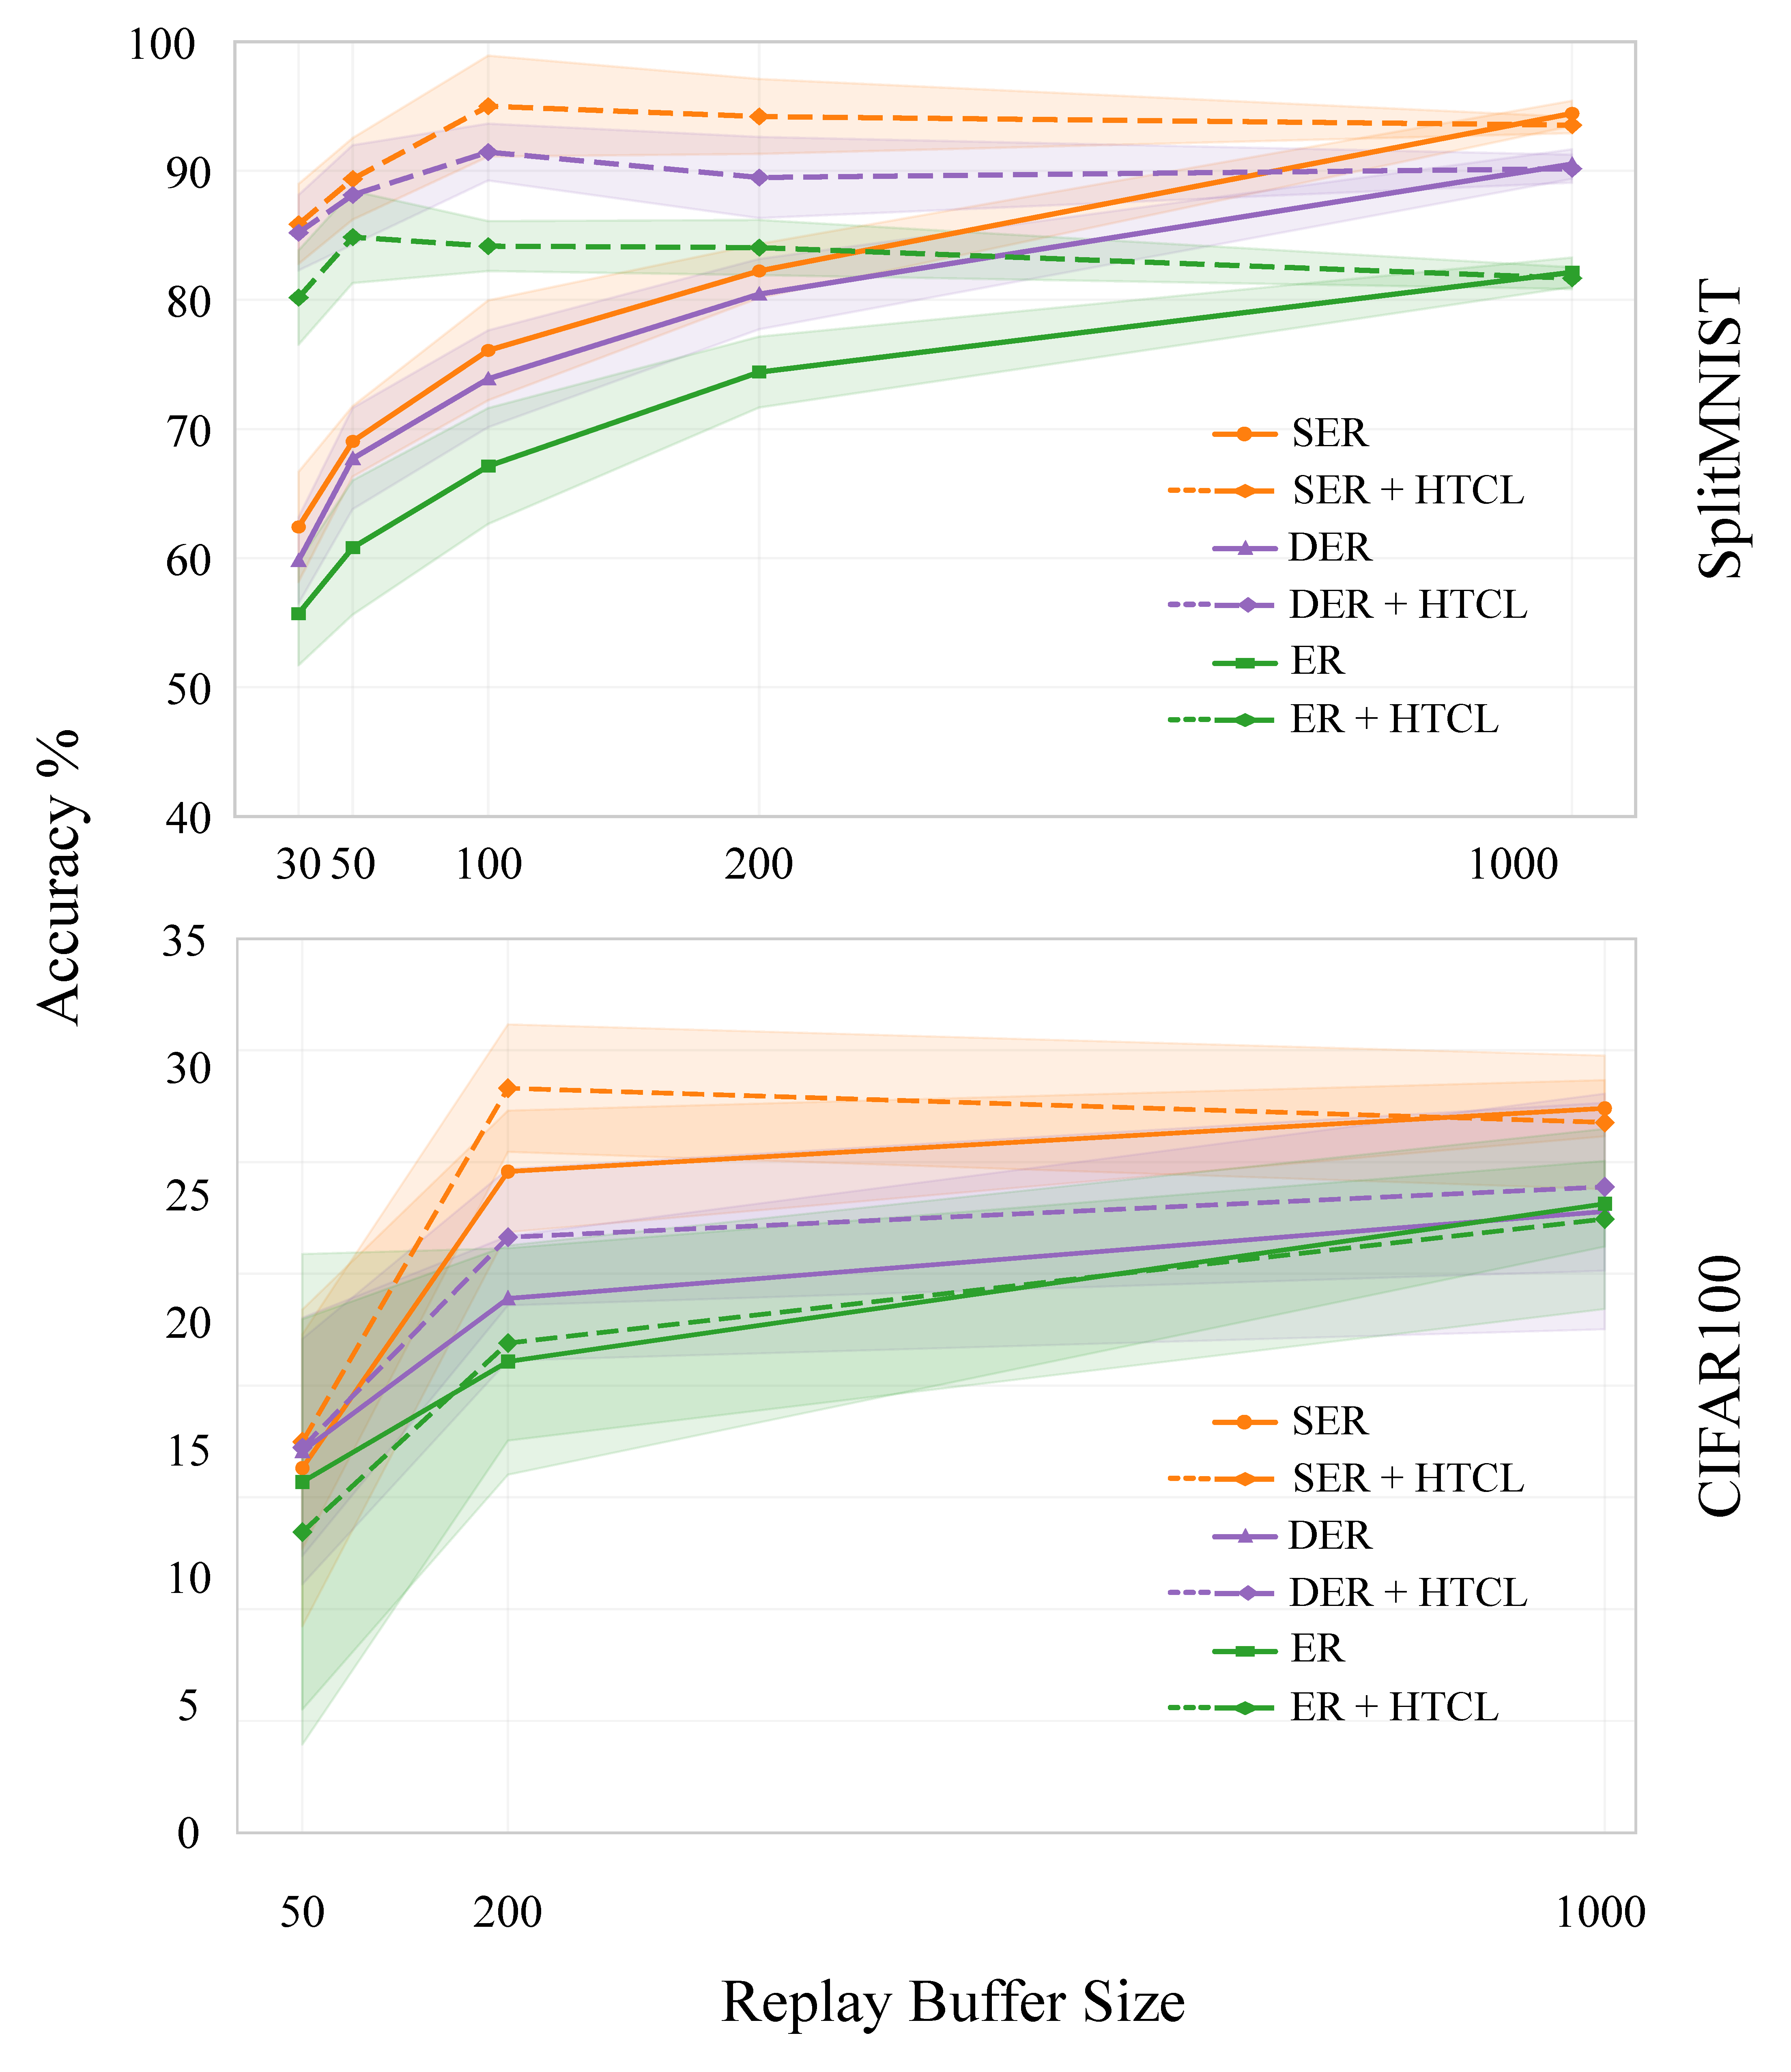
\includegraphics[width=\columnwidth]{figures/memory.pdf}
  \caption{\textbf{Effect of replay buffer size on SplitMNIST and Split CIFAR-100.} ER, DER, and SER with and without HTCL across buffer capacities. HTCL gains are largest under small buffers, where curvature-aware consolidation compensates for limited rehearsal; the relative advantage shrinks as the buffer approaches joint-training capacity.}
    \label{fig:memory}
\end{figure}

Replay-based CL methods rely heavily on buffer capacity. When replay memory is sufficiently large, rehearsal can approximate joint training and substantially mitigate forgetting. However, in realistic low-memory regimes, replay becomes much less reliable. To evaluate the robustness of HTCL under such constraints, we conduct experiments on both SplitMNIST and Split CIFAR-100 while varying the replay buffer size. For SplitMNIST, we sweep buffer sizes in $\{30, 50, 100, 200, 500\}$, whereas for Split CIFAR-100 we evaluate buffers of size $50$, $200$, and $1000$ to reflect the substantially larger number of classes.

Figure~\ref{fig:memory} reports the performance of ER, DER, and SER, together with their HTCL-augmented variants. Under very small buffers, standalone replay baselines exhibit severe forgetting due to insufficient coverage of previously learned tasks. In contrast, HTCL-enhanced models (ER+HTCL, DER+HTCL, SER+HTCL) consistently achieve higher accuracy, demonstrating that curvature-aware consolidation compensates for limited rehearsal by providing additional stability.

As buffer capacity increases, the performance gap between the baselines and their HTCL-augmented counterparts narrows. On SplitMNIST, replay approximates joint training once the buffer reaches moderate size, at which point model capacity becomes the dominant limiting factor and HTCL offers only marginal improvements. On Split CIFAR-100, extremely small buffers (e.g., 50 samples) produce unstable and low-quality performance, reflecting the insufficiency of such memory to represent 100 classes. Increasing the buffer to 200 yields a substantial improvement, and further increasing it to 1000 reduces the benefits of HTCL, mirroring the saturation observed in SplitMNIST.

These results confirm that HTCL is particularly advantageous in low-memory regimes: it acts as a complementary stabilization mechanism that mitigates forgetting when replay alone is inadequate, while remaining lightweight enough to avoid hindering performance when memory is plentiful.

\subsection{Relation to Federated Aggregation Methods}
\label{app:federated}

Although HTCL shares a structural similarity with federated learning methods, their objectives and use-cases are very different. Both maintain multiple models and periodically consolidate their updates into a single global model. For completeness and to evaluate these approaches for their ability to consolidate performance across tasks, we compared HTCL against two widely used federated baselines, FedAvg~\cite{mcmahan2017communication} and FedProx~\cite{li2020federated}. 

\begin{figure}[!t]
  \centering
  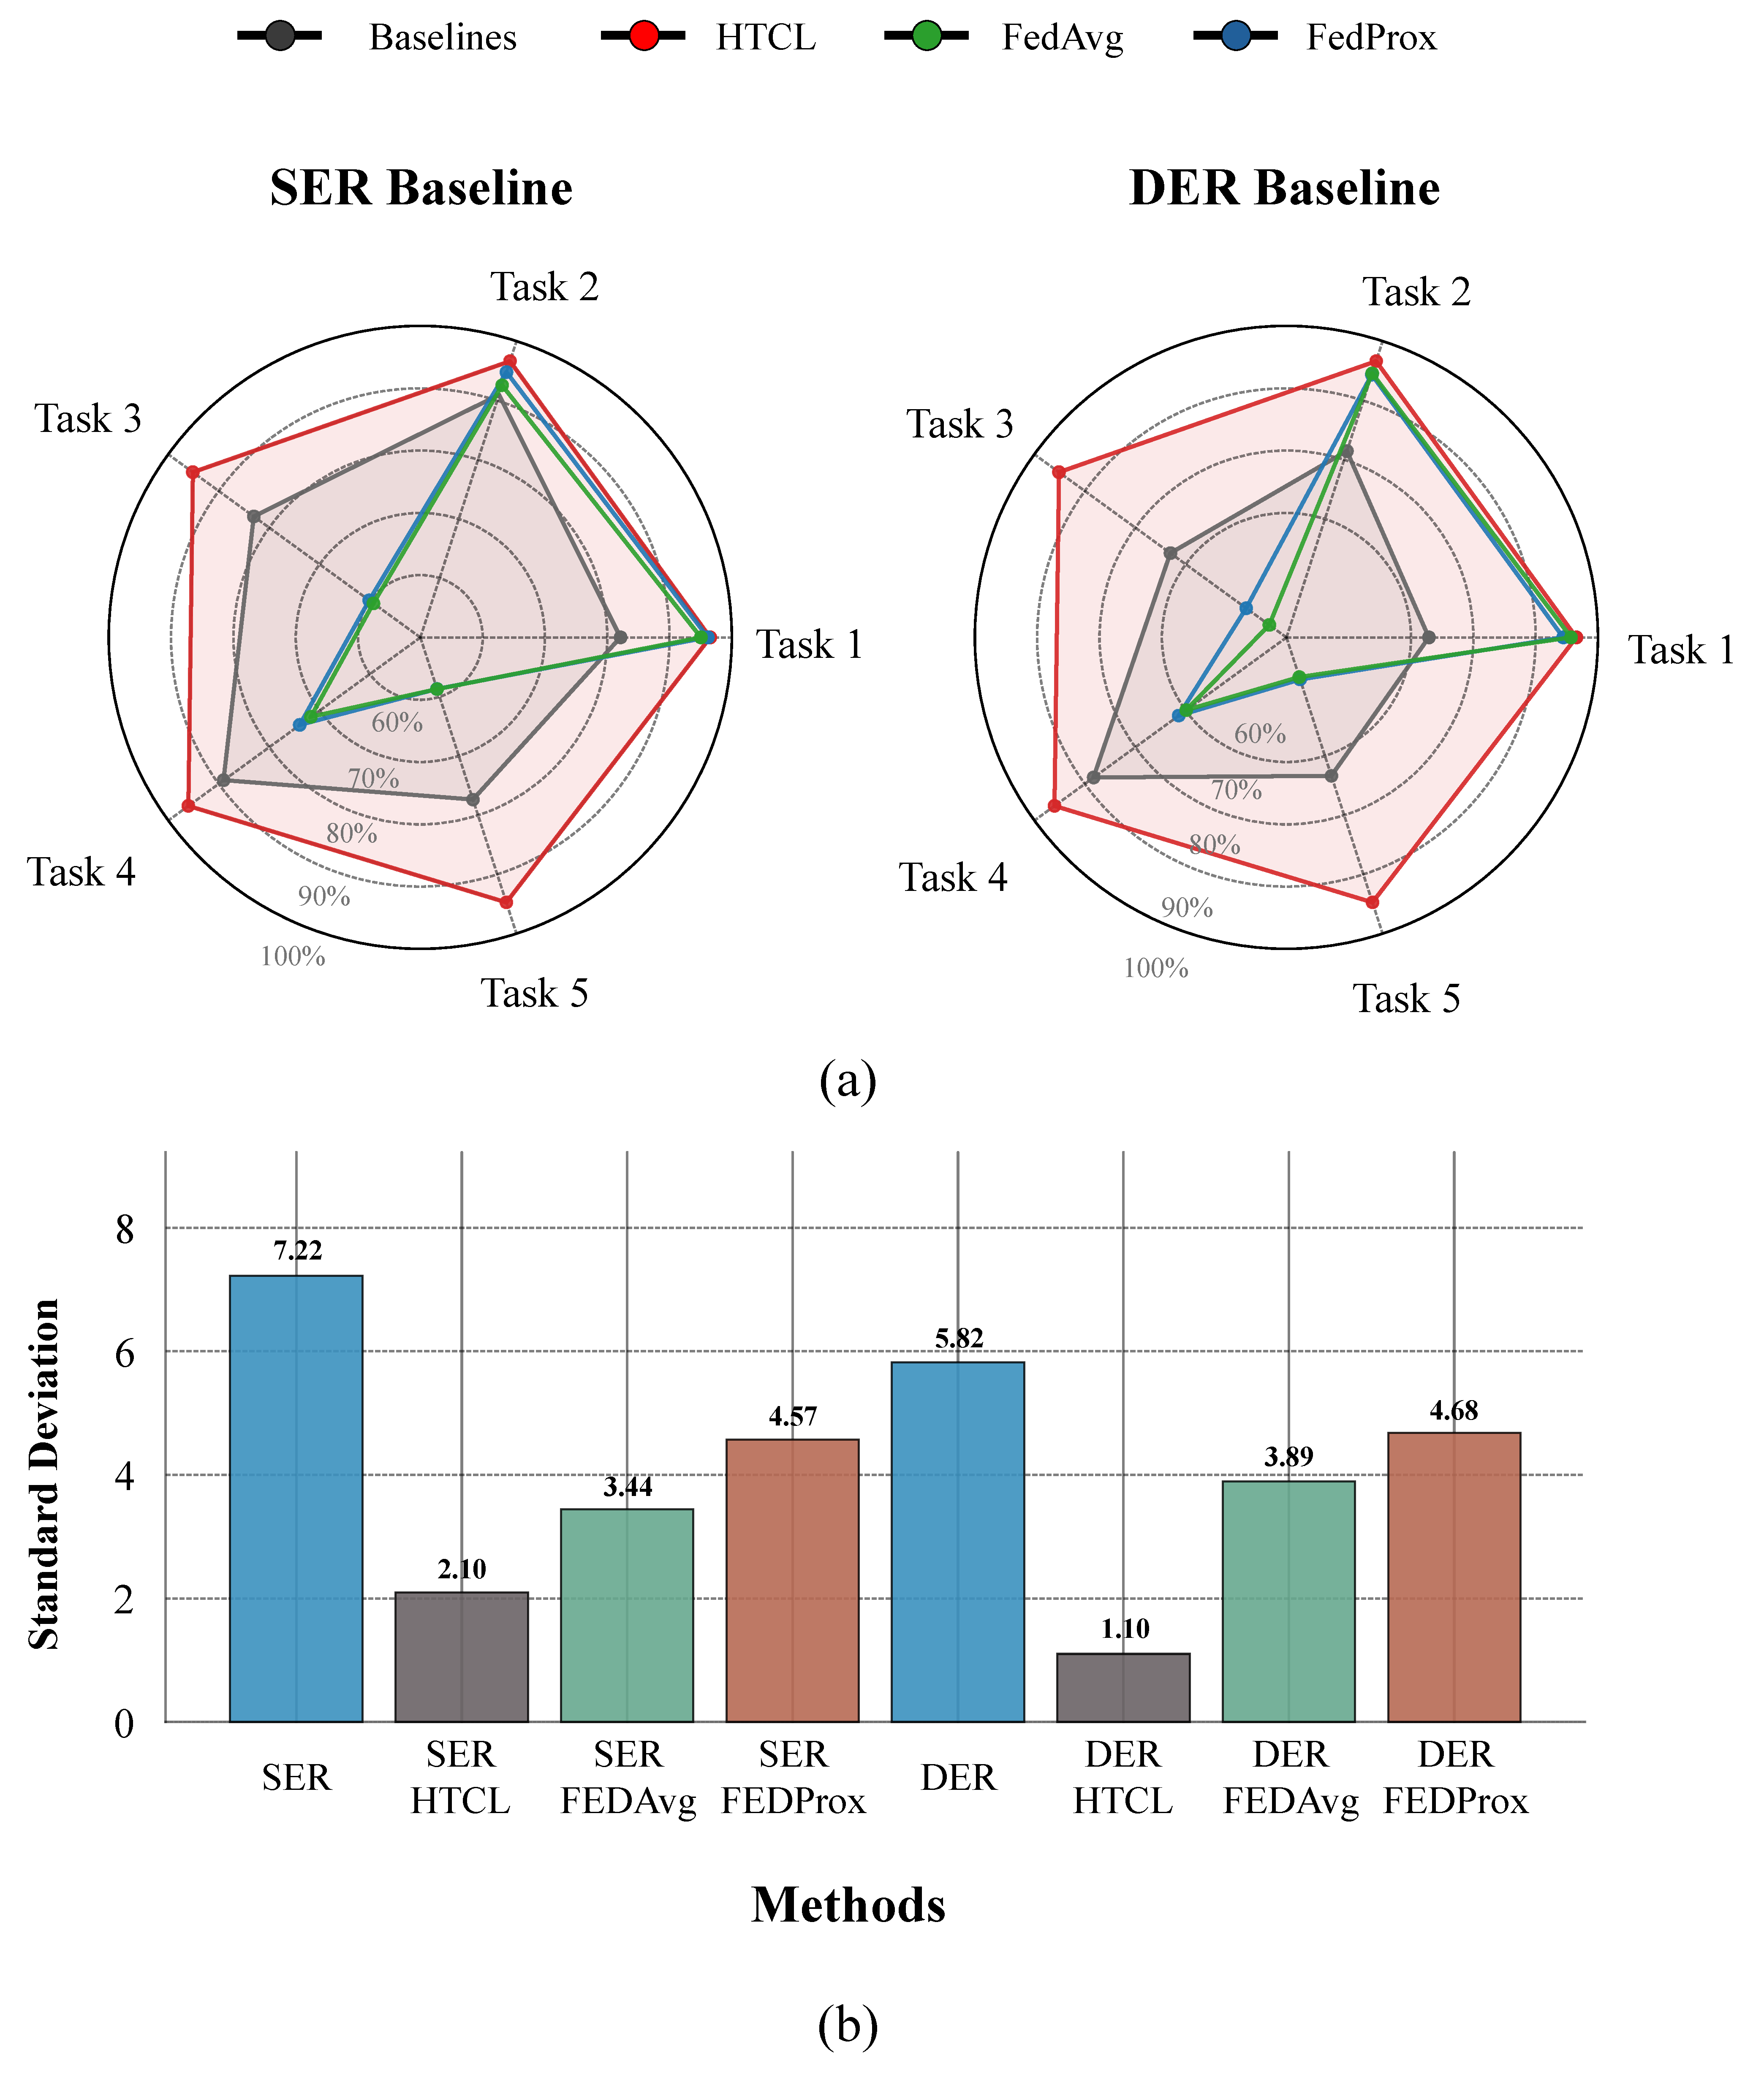
\includegraphics[width=\columnwidth]{figures/updated_figures/radar.pdf}
  \caption{\textbf{Comparison of HTCL with federated learning baselines.} Local models are trained using SER and DER on SplitMNIST, followed by global consolidation using HTCL, FedAvg, or FedProx. SER and DER without consolidation serve as baselines. (a) HTCL achieves consistently balanced accuracy across all tasks, whereas FedAvg and FedProx attain higher accuracy on some tasks at the expense of others. (b) Standard deviation across task permutations shows that HTCL provides the strongest reduction in task-order sensitivity compared to federated baselines.}
    \label{fig:fed-comp}
\end{figure}

\textbf{Experimental setup.} In our experiment, we treat each task in the continual learning sequence as analogous to a federated client. For each task, we first train a local model using either SER or DER as the base continual learning method. After training on each task, we update a global model using one of three consolidation strategies. These are HTCL, FedAvg, or FedProx. We then evaluate the final global model on all tasks and measure both accuracy and sensitivity to task ordering.

\textbf{Balanced performance across tasks.} Figure~\ref{fig:fed-comp}(a) shows per-task accuracy on SplitMNIST. FedAvg and FedProx achieve high accuracy on some tasks but at the cost of degraded performance on others. This uneven pattern suggests that simple averaging or proximal regularization does not account for the sequential structure of continual learning. HTCL achieves more balanced performance across all five tasks. 

\textbf{Task-order robustness.} Figure~\ref{fig:fed-comp}(b) compares the standard deviation of accuracy across different task orderings. Both FedAvg and FedProx reduce variance compared to the raw SER and DER baselines, indicating some degree of stabilization. However, HTCL achieves the lowest standard deviation overall. This difference highlights a fundamental distinction between the two settings. Federated methods dampen update magnitudes through averaging or regularization. HTCL instead consolidates knowledge using second-order information that is tailored to sequential, temporal learning.

\section{Limitations}
\label{app:limitation}
HTCL inherits two practical constraints from its design. First, intra-group permutation search scales as $k!$, restricting useful group sizes to $k < 5$; the empirical break-even on SplitMNIST occurs at $k = 3$ (Appendix~\ref{app:break-even-point}), beyond which additional compute yields negligible accuracy gains. Second, the closed-form update in Eq. (6) requires inverting a $d \times d$ Hessian and is intractable at modern model scales, so all reported results use diagonal or low-rank curvature approximations. The accuracy of these approximations near saddle regions of the loss landscape is not characterized in this work. Wall-clock cost also grows roughly $4\times$ relative to the underlying baseline at $L=2$, which may be prohibitive for latency-bounded continual deployments.




\section*{Acknowledgment}
Funding and acknowledgments to be added.

\bibliographystyle{IEEEtran}
\bibliography{IEEEabrv,references}

\end{document}
